\section{Results}
\label{hptpcPaper:sec:Results}

	%\begin{figure}[ht]
	%	\begin{minipage}[t]{0.48\textwidth}
	%		\centering
	%		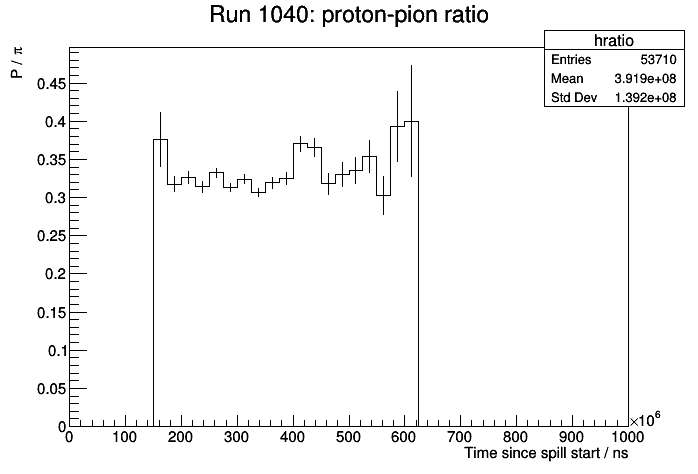
\includegraphics[width=\textwidth]{files/Figures/Run1040_proPiRatio}
	%		\caption{The ratio of protons to pions as a function of time since the start of the beam spill. For these data, 1 moderator block was in place and the beam momentum was nominally 0.8~GeV/c. The data for this graph is from the sum of 255 spills.}
	%		\label{fig:proPiRatio}
	%	\end{minipage} 
	%	\hspace{0.3cm}
	%	\begin{minipage}[t]{0.48\textwidth}
	%		\centering
	%		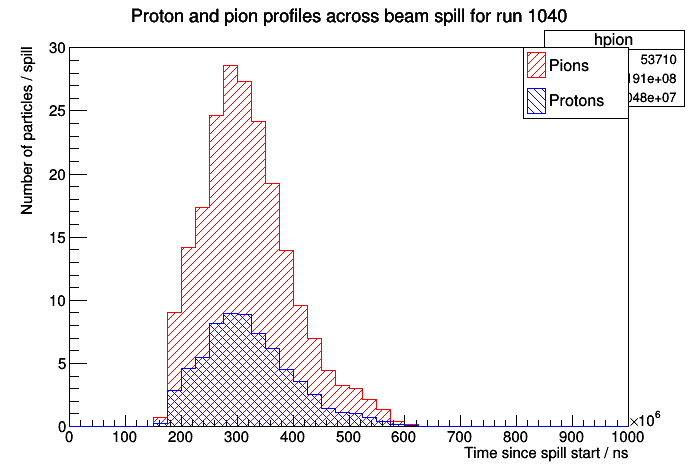
\includegraphics[width=\textwidth]{files/Figures/Run1040_proPiProf}
	%		\caption{The number of protons and pions detected per spill by the DsToF as a function of time since the start of the beam spill. For these data, 1 moderator block was in place and the beam momentum was nominally 0.8~GeV/c. The data for this graph is from the sum of 255 spills.}
	%		\label{fig:proPiProf}
	%	\end{minipage}
	%\end{figure}
   
   	\begin{figure}[ht]
   		\begin{minipage}[t]{0.48\textwidth}
   			\begin{adjustbox}{max totalsize={\textwidth}{.35\textheight},center}
		   		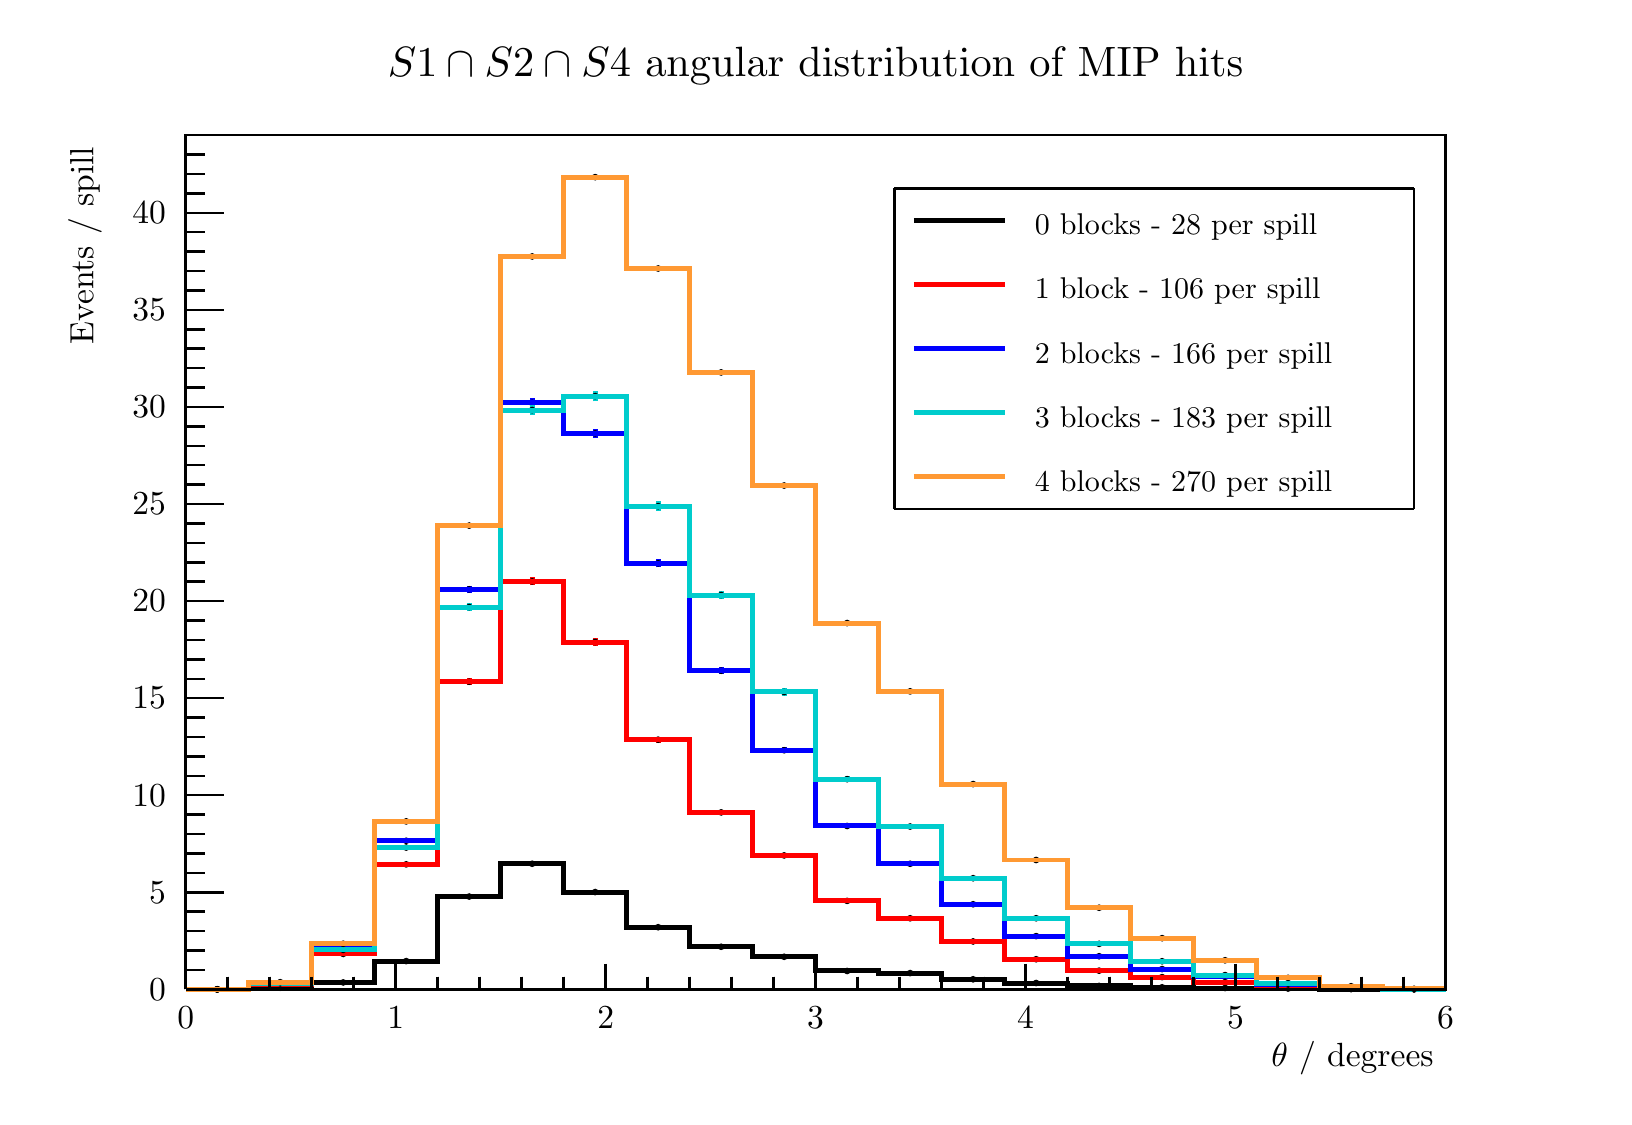
\begin{tikzpicture}
\pgfdeclareplotmark{cross} {
\pgfpathmoveto{\pgfpoint{-0.3\pgfplotmarksize}{\pgfplotmarksize}}
\pgfpathlineto{\pgfpoint{+0.3\pgfplotmarksize}{\pgfplotmarksize}}
\pgfpathlineto{\pgfpoint{+0.3\pgfplotmarksize}{0.3\pgfplotmarksize}}
\pgfpathlineto{\pgfpoint{+1\pgfplotmarksize}{0.3\pgfplotmarksize}}
\pgfpathlineto{\pgfpoint{+1\pgfplotmarksize}{-0.3\pgfplotmarksize}}
\pgfpathlineto{\pgfpoint{+0.3\pgfplotmarksize}{-0.3\pgfplotmarksize}}
\pgfpathlineto{\pgfpoint{+0.3\pgfplotmarksize}{-1.\pgfplotmarksize}}
\pgfpathlineto{\pgfpoint{-0.3\pgfplotmarksize}{-1.\pgfplotmarksize}}
\pgfpathlineto{\pgfpoint{-0.3\pgfplotmarksize}{-0.3\pgfplotmarksize}}
\pgfpathlineto{\pgfpoint{-1.\pgfplotmarksize}{-0.3\pgfplotmarksize}}
\pgfpathlineto{\pgfpoint{-1.\pgfplotmarksize}{0.3\pgfplotmarksize}}
\pgfpathlineto{\pgfpoint{-0.3\pgfplotmarksize}{0.3\pgfplotmarksize}}
\pgfpathclose
\pgfusepathqstroke
}
\pgfdeclareplotmark{cross*} {
\pgfpathmoveto{\pgfpoint{-0.3\pgfplotmarksize}{\pgfplotmarksize}}
\pgfpathlineto{\pgfpoint{+0.3\pgfplotmarksize}{\pgfplotmarksize}}
\pgfpathlineto{\pgfpoint{+0.3\pgfplotmarksize}{0.3\pgfplotmarksize}}
\pgfpathlineto{\pgfpoint{+1\pgfplotmarksize}{0.3\pgfplotmarksize}}
\pgfpathlineto{\pgfpoint{+1\pgfplotmarksize}{-0.3\pgfplotmarksize}}
\pgfpathlineto{\pgfpoint{+0.3\pgfplotmarksize}{-0.3\pgfplotmarksize}}
\pgfpathlineto{\pgfpoint{+0.3\pgfplotmarksize}{-1.\pgfplotmarksize}}
\pgfpathlineto{\pgfpoint{-0.3\pgfplotmarksize}{-1.\pgfplotmarksize}}
\pgfpathlineto{\pgfpoint{-0.3\pgfplotmarksize}{-0.3\pgfplotmarksize}}
\pgfpathlineto{\pgfpoint{-1.\pgfplotmarksize}{-0.3\pgfplotmarksize}}
\pgfpathlineto{\pgfpoint{-1.\pgfplotmarksize}{0.3\pgfplotmarksize}}
\pgfpathlineto{\pgfpoint{-0.3\pgfplotmarksize}{0.3\pgfplotmarksize}}
\pgfpathclose
\pgfusepathqfillstroke
}
\pgfdeclareplotmark{newstar} {
\pgfpathmoveto{\pgfqpoint{0pt}{\pgfplotmarksize}}
\pgfpathlineto{\pgfqpointpolar{44}{0.5\pgfplotmarksize}}
\pgfpathlineto{\pgfqpointpolar{18}{\pgfplotmarksize}}
\pgfpathlineto{\pgfqpointpolar{-20}{0.5\pgfplotmarksize}}
\pgfpathlineto{\pgfqpointpolar{-54}{\pgfplotmarksize}}
\pgfpathlineto{\pgfqpointpolar{-90}{0.5\pgfplotmarksize}}
\pgfpathlineto{\pgfqpointpolar{234}{\pgfplotmarksize}}
\pgfpathlineto{\pgfqpointpolar{198}{0.5\pgfplotmarksize}}
\pgfpathlineto{\pgfqpointpolar{162}{\pgfplotmarksize}}
\pgfpathlineto{\pgfqpointpolar{134}{0.5\pgfplotmarksize}}
\pgfpathclose
\pgfusepathqstroke
}
\pgfdeclareplotmark{newstar*} {
\pgfpathmoveto{\pgfqpoint{0pt}{\pgfplotmarksize}}
\pgfpathlineto{\pgfqpointpolar{44}{0.5\pgfplotmarksize}}
\pgfpathlineto{\pgfqpointpolar{18}{\pgfplotmarksize}}
\pgfpathlineto{\pgfqpointpolar{-20}{0.5\pgfplotmarksize}}
\pgfpathlineto{\pgfqpointpolar{-54}{\pgfplotmarksize}}
\pgfpathlineto{\pgfqpointpolar{-90}{0.5\pgfplotmarksize}}
\pgfpathlineto{\pgfqpointpolar{234}{\pgfplotmarksize}}
\pgfpathlineto{\pgfqpointpolar{198}{0.5\pgfplotmarksize}}
\pgfpathlineto{\pgfqpointpolar{162}{\pgfplotmarksize}}
\pgfpathlineto{\pgfqpointpolar{134}{0.5\pgfplotmarksize}}
\pgfpathclose
\pgfusepathqfillstroke
}
\definecolor{c}{rgb}{1,1,1};
\draw [color=c, fill=c] (0,0) rectangle (20,13.5632);
\draw [color=c, fill=c] (2,1.35632) rectangle (18,12.2069);
\definecolor{c}{rgb}{0,0,0};
\draw [c,line width=0.9] (2,1.35632) -- (2,12.2069) -- (18,12.2069) -- (18,1.35632) -- (2,1.35632);
\definecolor{c}{rgb}{1,1,1};
\draw [color=c, fill=c] (2,1.35632) rectangle (18,12.2069);
\definecolor{c}{rgb}{0,0,0};
\draw [c,line width=0.9] (2,1.35632) -- (2,12.2069) -- (18,12.2069) -- (18,1.35632) -- (2,1.35632);
\definecolor{c}{rgb}{0,0,0.6};
\draw [c,line width=0.9] (2,1.35632) -- (2.8,1.35632) -- (2.8,1.35632) -- (3.6,1.35632) -- (3.6,1.35632) -- (4.4,1.35632) -- (4.4,1.35632) -- (5.2,1.35632) -- (5.2,1.35632) -- (6,1.35632) -- (6,1.35632) -- (6.8,1.35632) -- (6.8,1.35632) --
 (7.6,1.35632) -- (7.6,1.35632) -- (8.4,1.35632) -- (8.4,1.35632) -- (9.2,1.35632) -- (9.2,1.35632) -- (10,1.35632) -- (10,1.35632) -- (10.8,1.35632) -- (10.8,1.35632) -- (11.6,1.35632) -- (11.6,1.35632) -- (12.4,1.35632) -- (12.4,1.35632) --
 (13.2,1.35632) -- (13.2,1.35632) -- (14,1.35632) -- (14,1.35632) -- (14.8,1.35632) -- (14.8,1.35632) -- (15.6,1.35632) -- (15.6,1.35632) -- (16.4,1.35632) -- (16.4,1.35632) -- (17.2,1.35632) -- (17.2,1.35632) -- (18,1.35632);
\definecolor{c}{rgb}{0,0,0};
\draw [c,line width=0.9] (2,1.35632) -- (18,1.35632);
\draw [anchor= east] (18,0.488276) node[scale=1.2126, color=c, rotate=0]{$\theta$ / degrees};
\draw [c,line width=0.9] (2,1.68184) -- (2,1.35632);
\draw [c,line width=0.9] (2.53333,1.51908) -- (2.53333,1.35632);
\draw [c,line width=0.9] (3.06667,1.51908) -- (3.06667,1.35632);
\draw [c,line width=0.9] (3.6,1.51908) -- (3.6,1.35632);
\draw [c,line width=0.9] (4.13333,1.51908) -- (4.13333,1.35632);
\draw [c,line width=0.9] (4.66667,1.68184) -- (4.66667,1.35632);
\draw [c,line width=0.9] (5.2,1.51908) -- (5.2,1.35632);
\draw [c,line width=0.9] (5.73333,1.51908) -- (5.73333,1.35632);
\draw [c,line width=0.9] (6.26667,1.51908) -- (6.26667,1.35632);
\draw [c,line width=0.9] (6.8,1.51908) -- (6.8,1.35632);
\draw [c,line width=0.9] (7.33333,1.68184) -- (7.33333,1.35632);
\draw [c,line width=0.9] (7.86667,1.51908) -- (7.86667,1.35632);
\draw [c,line width=0.9] (8.4,1.51908) -- (8.4,1.35632);
\draw [c,line width=0.9] (8.93333,1.51908) -- (8.93333,1.35632);
\draw [c,line width=0.9] (9.46667,1.51908) -- (9.46667,1.35632);
\draw [c,line width=0.9] (10,1.68184) -- (10,1.35632);
\draw [c,line width=0.9] (10.5333,1.51908) -- (10.5333,1.35632);
\draw [c,line width=0.9] (11.0667,1.51908) -- (11.0667,1.35632);
\draw [c,line width=0.9] (11.6,1.51908) -- (11.6,1.35632);
\draw [c,line width=0.9] (12.1333,1.51908) -- (12.1333,1.35632);
\draw [c,line width=0.9] (12.6667,1.68184) -- (12.6667,1.35632);
\draw [c,line width=0.9] (13.2,1.51908) -- (13.2,1.35632);
\draw [c,line width=0.9] (13.7333,1.51908) -- (13.7333,1.35632);
\draw [c,line width=0.9] (14.2667,1.51908) -- (14.2667,1.35632);
\draw [c,line width=0.9] (14.8,1.51908) -- (14.8,1.35632);
\draw [c,line width=0.9] (15.3333,1.68184) -- (15.3333,1.35632);
\draw [c,line width=0.9] (15.8667,1.51908) -- (15.8667,1.35632);
\draw [c,line width=0.9] (16.4,1.51908) -- (16.4,1.35632);
\draw [c,line width=0.9] (16.9333,1.51908) -- (16.9333,1.35632);
\draw [c,line width=0.9] (17.4667,1.51908) -- (17.4667,1.35632);
\draw [c,line width=0.9] (18,1.68184) -- (18,1.35632);
\draw [anchor=base] (2,0.854483) node[scale=1.2126, color=c, rotate=0]{0};
\draw [anchor=base] (4.66667,0.854483) node[scale=1.2126, color=c, rotate=0]{1};
\draw [anchor=base] (7.33333,0.854483) node[scale=1.2126, color=c, rotate=0]{2};
\draw [anchor=base] (10,0.854483) node[scale=1.2126, color=c, rotate=0]{3};
\draw [anchor=base] (12.6667,0.854483) node[scale=1.2126, color=c, rotate=0]{4};
\draw [anchor=base] (15.3333,0.854483) node[scale=1.2126, color=c, rotate=0]{5};
\draw [anchor=base] (18,0.854483) node[scale=1.2126, color=c, rotate=0]{6};
\draw [c,line width=0.9] (2,1.35632) -- (2,12.2069);
\draw [anchor= east] (0.72,12.2069) node[scale=1.2126, color=c, rotate=90]{ Events / spill};
\draw [c,line width=0.9] (2.48,1.35632) -- (2,1.35632);
\draw [c,line width=0.9] (2.24,1.60289) -- (2,1.60289);
\draw [c,line width=0.9] (2.24,1.84945) -- (2,1.84945);
\draw [c,line width=0.9] (2.24,2.09602) -- (2,2.09602);
\draw [c,line width=0.9] (2.24,2.34258) -- (2,2.34258);
\draw [c,line width=0.9] (2.48,2.58915) -- (2,2.58915);
\draw [c,line width=0.9] (2.24,2.83571) -- (2,2.83571);
\draw [c,line width=0.9] (2.24,3.08228) -- (2,3.08228);
\draw [c,line width=0.9] (2.24,3.32884) -- (2,3.32884);
\draw [c,line width=0.9] (2.24,3.57541) -- (2,3.57541);
\draw [c,line width=0.9] (2.48,3.82197) -- (2,3.82197);
\draw [c,line width=0.9] (2.24,4.06854) -- (2,4.06854);
\draw [c,line width=0.9] (2.24,4.31511) -- (2,4.31511);
\draw [c,line width=0.9] (2.24,4.56167) -- (2,4.56167);
\draw [c,line width=0.9] (2.24,4.80824) -- (2,4.80824);
\draw [c,line width=0.9] (2.48,5.0548) -- (2,5.0548);
\draw [c,line width=0.9] (2.24,5.30137) -- (2,5.30137);
\draw [c,line width=0.9] (2.24,5.54793) -- (2,5.54793);
\draw [c,line width=0.9] (2.24,5.7945) -- (2,5.7945);
\draw [c,line width=0.9] (2.24,6.04106) -- (2,6.04106);
\draw [c,line width=0.9] (2.48,6.28763) -- (2,6.28763);
\draw [c,line width=0.9] (2.24,6.53419) -- (2,6.53419);
\draw [c,line width=0.9] (2.24,6.78076) -- (2,6.78076);
\draw [c,line width=0.9] (2.24,7.02732) -- (2,7.02732);
\draw [c,line width=0.9] (2.24,7.27389) -- (2,7.27389);
\draw [c,line width=0.9] (2.48,7.52045) -- (2,7.52045);
\draw [c,line width=0.9] (2.24,7.76702) -- (2,7.76702);
\draw [c,line width=0.9] (2.24,8.01359) -- (2,8.01359);
\draw [c,line width=0.9] (2.24,8.26015) -- (2,8.26015);
\draw [c,line width=0.9] (2.24,8.50672) -- (2,8.50672);
\draw [c,line width=0.9] (2.48,8.75328) -- (2,8.75328);
\draw [c,line width=0.9] (2.24,8.99985) -- (2,8.99985);
\draw [c,line width=0.9] (2.24,9.24641) -- (2,9.24641);
\draw [c,line width=0.9] (2.24,9.49298) -- (2,9.49298);
\draw [c,line width=0.9] (2.24,9.73954) -- (2,9.73954);
\draw [c,line width=0.9] (2.48,9.98611) -- (2,9.98611);
\draw [c,line width=0.9] (2.24,10.2327) -- (2,10.2327);
\draw [c,line width=0.9] (2.24,10.4792) -- (2,10.4792);
\draw [c,line width=0.9] (2.24,10.7258) -- (2,10.7258);
\draw [c,line width=0.9] (2.24,10.9724) -- (2,10.9724);
\draw [c,line width=0.9] (2.48,11.2189) -- (2,11.2189);
\draw [c,line width=0.9] (2.48,11.2189) -- (2,11.2189);
\draw [c,line width=0.9] (2.24,11.4655) -- (2,11.4655);
\draw [c,line width=0.9] (2.24,11.7121) -- (2,11.7121);
\draw [c,line width=0.9] (2.24,11.9586) -- (2,11.9586);
\draw [c,line width=0.9] (2.24,12.2052) -- (2,12.2052);
\draw [anchor= east] (1.9,1.35632) node[scale=1.2126, color=c, rotate=0]{0};
\draw [anchor= east] (1.9,2.58915) node[scale=1.2126, color=c, rotate=0]{5};
\draw [anchor= east] (1.9,3.82197) node[scale=1.2126, color=c, rotate=0]{10};
\draw [anchor= east] (1.9,5.0548) node[scale=1.2126, color=c, rotate=0]{15};
\draw [anchor= east] (1.9,6.28763) node[scale=1.2126, color=c, rotate=0]{20};
\draw [anchor= east] (1.9,7.52045) node[scale=1.2126, color=c, rotate=0]{25};
\draw [anchor= east] (1.9,8.75328) node[scale=1.2126, color=c, rotate=0]{30};
\draw [anchor= east] (1.9,9.98611) node[scale=1.2126, color=c, rotate=0]{35};
\draw [anchor= east] (1.9,11.2189) node[scale=1.2126, color=c, rotate=0]{40};
\draw [c,line width=1.8] (2.4,1.35632) -- (2.4,1.35667);
\draw [c,line width=1.8] (2.4,1.35667) -- (2.4,1.35701);
\foreach \P in {(2.4,1.35667)}{\draw[mark options={color=c,fill=c},mark size=2.402402pt,mark=*,mark size=1pt] plot coordinates {\P};}
\draw [c,line width=1.8] (3.2,1.37421) -- (3.2,1.37732);
\draw [c,line width=1.8] (3.2,1.37732) -- (3.2,1.38043);
\foreach \P in {(3.2,1.37732)}{\draw[mark options={color=c,fill=c},mark size=2.402402pt,mark=*,mark size=1pt] plot coordinates {\P};}
\draw [c,line width=1.8] (4,1.43826) -- (4,1.44474);
\draw [c,line width=1.8] (4,1.44474) -- (4,1.45123);
\foreach \P in {(4,1.44474)}{\draw[mark options={color=c,fill=c},mark size=2.402402pt,mark=*,mark size=1pt] plot coordinates {\P};}
\draw [c,line width=1.8] (4.8,1.70111) -- (4.8,1.71559);
\draw [c,line width=1.8] (4.8,1.71559) -- (4.8,1.73006);
\foreach \P in {(4.8,1.71559)}{\draw[mark options={color=c,fill=c},mark size=2.402402pt,mark=*,mark size=1pt] plot coordinates {\P};}
\draw [c,line width=1.8] (5.6,2.50801) -- (5.6,2.53547);
\draw [c,line width=1.8] (5.6,2.53547) -- (5.6,2.56293);
\foreach \P in {(5.6,2.53547)}{\draw[mark options={color=c,fill=c},mark size=2.402402pt,mark=*,mark size=1pt] plot coordinates {\P};}
\draw [c,line width=1.8] (6.4,2.91977) -- (6.4,2.95217);
\draw [c,line width=1.8] (6.4,2.95217) -- (6.4,2.98457);
\foreach \P in {(6.4,2.95217)}{\draw[mark options={color=c,fill=c},mark size=2.402402pt,mark=*,mark size=1pt] plot coordinates {\P};}
\draw [c,line width=1.8] (7.2,2.56376) -- (7.2,2.59229);
\draw [c,line width=1.8] (7.2,2.59229) -- (7.2,2.62081);
\foreach \P in {(7.2,2.59229)}{\draw[mark options={color=c,fill=c},mark size=2.402402pt,mark=*,mark size=1pt] plot coordinates {\P};}
\draw [c,line width=1.8] (8,2.12349) -- (8,2.14597);
\draw [c,line width=1.8] (8,2.14597) -- (8,2.16846);
\foreach \P in {(8,2.14597)}{\draw[mark options={color=c,fill=c},mark size=2.402402pt,mark=*,mark size=1pt] plot coordinates {\P};}
\draw [c,line width=1.8] (8.8,1.87945) -- (8.8,1.89768);
\draw [c,line width=1.8] (8.8,1.89768) -- (8.8,1.91591);
\foreach \P in {(8.8,1.89768)}{\draw[mark options={color=c,fill=c},mark size=2.402402pt,mark=*,mark size=1pt] plot coordinates {\P};}
\draw [c,line width=1.8] (9.6,1.75482) -- (9.6,1.77052);
\draw [c,line width=1.8] (9.6,1.77052) -- (9.6,1.78623);
\foreach \P in {(9.6,1.77052)}{\draw[mark options={color=c,fill=c},mark size=2.402402pt,mark=*,mark size=1pt] plot coordinates {\P};}
\draw [c,line width=1.8] (10.4,1.57888) -- (10.4,1.59008);
\draw [c,line width=1.8] (10.4,1.59008) -- (10.4,1.60128);
\foreach \P in {(10.4,1.59008)}{\draw[mark options={color=c,fill=c},mark size=2.402402pt,mark=*,mark size=1pt] plot coordinates {\P};}
\draw [c,line width=1.8] (11.2,1.55242) -- (11.2,1.56325);
\draw [c,line width=1.8] (11.2,1.56325) -- (11.2,1.57407);
\foreach \P in {(11.2,1.56325)}{\draw[mark options={color=c,fill=c},mark size=2.402402pt,mark=*,mark size=1pt] plot coordinates {\P};}
\draw [c,line width=1.8] (12,1.4762) -- (12,1.48457);
\draw [c,line width=1.8] (12,1.48457) -- (12,1.49294);
\foreach \P in {(12,1.48457)}{\draw[mark options={color=c,fill=c},mark size=2.402402pt,mark=*,mark size=1pt] plot coordinates {\P};}
\draw [c,line width=1.8] (12.8,1.43085) -- (12.8,1.43719);
\draw [c,line width=1.8] (12.8,1.43719) -- (12.8,1.44352);
\foreach \P in {(12.8,1.43719)}{\draw[mark options={color=c,fill=c},mark size=2.402402pt,mark=*,mark size=1pt] plot coordinates {\P};}
\draw [c,line width=1.8] (13.6,1.396) -- (13.6,1.40053);
\draw [c,line width=1.8] (13.6,1.40053) -- (13.6,1.40507);
\foreach \P in {(13.6,1.40053)}{\draw[mark options={color=c,fill=c},mark size=2.402402pt,mark=*,mark size=1pt] plot coordinates {\P};}
\draw [c,line width=1.8] (14.4,1.3793) -- (14.4,1.38292);
\draw [c,line width=1.8] (14.4,1.38292) -- (14.4,1.38654);
\foreach \P in {(14.4,1.38292)}{\draw[mark options={color=c,fill=c},mark size=2.402402pt,mark=*,mark size=1pt] plot coordinates {\P};}
\draw [c,line width=1.8] (15.2,1.37113) -- (15.2,1.37379);
\draw [c,line width=1.8] (15.2,1.37379) -- (15.2,1.37645);
\foreach \P in {(15.2,1.37379)}{\draw[mark options={color=c,fill=c},mark size=2.402402pt,mark=*,mark size=1pt] plot coordinates {\P};}
\draw [c,line width=1.8] (16,1.3653) -- (16,1.36731);
\draw [c,line width=1.8] (16,1.36731) -- (16,1.36933);
\foreach \P in {(16,1.36731)}{\draw[mark options={color=c,fill=c},mark size=2.402402pt,mark=*,mark size=1pt] plot coordinates {\P};}
\draw [c,line width=1.8] (16.8,1.35901) -- (16.8,1.36043);
\draw [c,line width=1.8] (16.8,1.36043) -- (16.8,1.36184);
\foreach \P in {(16.8,1.36043)}{\draw[mark options={color=c,fill=c},mark size=2.402402pt,mark=*,mark size=1pt] plot coordinates {\P};}
\draw [c,line width=1.8] (2,1.35632) -- (2.8,1.35632) -- (2.8,1.37732) -- (3.6,1.37732) -- (3.6,1.44474) -- (4.4,1.44474) -- (4.4,1.71559) -- (5.2,1.71559) -- (5.2,2.53547) -- (6,2.53547) -- (6,2.95217) -- (6.8,2.95217) -- (6.8,2.59229) --
 (7.6,2.59229) -- (7.6,2.14597) -- (8.4,2.14597) -- (8.4,1.89768) -- (9.2,1.89768) -- (9.2,1.77052) -- (10,1.77052) -- (10,1.59008) -- (10.8,1.59008) -- (10.8,1.56325) -- (11.6,1.56325) -- (11.6,1.48457) -- (12.4,1.48457) -- (12.4,1.43719) --
 (13.2,1.43719) -- (13.2,1.40053) -- (14,1.40053) -- (14,1.38292) -- (14.8,1.38292) -- (14.8,1.37379) -- (15.6,1.37379) -- (15.6,1.36731) -- (16.4,1.36731) -- (16.4,1.36043) -- (17.2,1.36043) -- (17.2,1.35632) -- (18,1.35632);
\definecolor{c}{rgb}{1,0,0};
\draw [c,line width=1.8] (2.4,1.35632) -- (2.4,1.35684);
\draw [c,line width=1.8] (2.4,1.35684) -- (2.4,1.35736);
\definecolor{c}{rgb}{0,0,0};
\foreach \P in {(2.4,1.35684)}{\draw[mark options={color=c,fill=c},mark size=2.402402pt,mark=*,mark size=1pt] plot coordinates {\P};}
\definecolor{c}{rgb}{1,0,0};
\draw [c,line width=1.8] (3.2,1.41399) -- (3.2,1.41942);
\draw [c,line width=1.8] (3.2,1.41942) -- (3.2,1.42485);
\definecolor{c}{rgb}{0,0,0};
\foreach \P in {(3.2,1.41942)}{\draw[mark options={color=c,fill=c},mark size=2.402402pt,mark=*,mark size=1pt] plot coordinates {\P};}
\definecolor{c}{rgb}{1,0,0};
\draw [c,line width=1.8] (4,1.79246) -- (4,1.8069);
\draw [c,line width=1.8] (4,1.8069) -- (4,1.82134);
\definecolor{c}{rgb}{0,0,0};
\foreach \P in {(4,1.8069)}{\draw[mark options={color=c,fill=c},mark size=2.402402pt,mark=*,mark size=1pt] plot coordinates {\P};}
\definecolor{c}{rgb}{1,0,0};
\draw [c,line width=1.8] (4.8,2.9168) -- (4.8,2.94435);
\draw [c,line width=1.8] (4.8,2.94435) -- (4.8,2.9719);
\definecolor{c}{rgb}{0,0,0};
\foreach \P in {(4.8,2.94435)}{\draw[mark options={color=c,fill=c},mark size=2.402402pt,mark=*,mark size=1pt] plot coordinates {\P};}
\definecolor{c}{rgb}{1,0,0};
\draw [c,line width=1.8] (5.6,5.21998) -- (5.6,5.26355);
\draw [c,line width=1.8] (5.6,5.26355) -- (5.6,5.30712);
\definecolor{c}{rgb}{0,0,0};
\foreach \P in {(5.6,5.26355)}{\draw[mark options={color=c,fill=c},mark size=2.402402pt,mark=*,mark size=1pt] plot coordinates {\P};}
\definecolor{c}{rgb}{1,0,0};
\draw [c,line width=1.8] (6.4,6.48763) -- (6.4,6.53825);
\draw [c,line width=1.8] (6.4,6.53825) -- (6.4,6.58887);
\definecolor{c}{rgb}{0,0,0};
\foreach \P in {(6.4,6.53825)}{\draw[mark options={color=c,fill=c},mark size=2.402402pt,mark=*,mark size=1pt] plot coordinates {\P};}
\definecolor{c}{rgb}{1,0,0};
\draw [c,line width=1.8] (7.2,5.7211) -- (7.2,5.76788);
\draw [c,line width=1.8] (7.2,5.76788) -- (7.2,5.81465);
\definecolor{c}{rgb}{0,0,0};
\foreach \P in {(7.2,5.76788)}{\draw[mark options={color=c,fill=c},mark size=2.402402pt,mark=*,mark size=1pt] plot coordinates {\P};}
\definecolor{c}{rgb}{1,0,0};
\draw [c,line width=1.8] (8,4.48824) -- (8,4.52785);
\draw [c,line width=1.8] (8,4.52785) -- (8,4.56745);
\definecolor{c}{rgb}{0,0,0};
\foreach \P in {(8,4.52785)}{\draw[mark options={color=c,fill=c},mark size=2.402402pt,mark=*,mark size=1pt] plot coordinates {\P};}
\definecolor{c}{rgb}{1,0,0};
\draw [c,line width=1.8] (8.8,3.57095) -- (8.8,3.60412);
\draw [c,line width=1.8] (8.8,3.60412) -- (8.8,3.63729);
\definecolor{c}{rgb}{0,0,0};
\foreach \P in {(8.8,3.60412)}{\draw[mark options={color=c,fill=c},mark size=2.402402pt,mark=*,mark size=1pt] plot coordinates {\P};}
\definecolor{c}{rgb}{1,0,0};
\draw [c,line width=1.8] (9.6,3.02904) -- (9.6,3.0578);
\draw [c,line width=1.8] (9.6,3.0578) -- (9.6,3.08655);
\definecolor{c}{rgb}{0,0,0};
\foreach \P in {(9.6,3.0578)}{\draw[mark options={color=c,fill=c},mark size=2.402402pt,mark=*,mark size=1pt] plot coordinates {\P};}
\definecolor{c}{rgb}{1,0,0};
\draw [c,line width=1.8] (10.4,2.45738) -- (10.4,2.48051);
\draw [c,line width=1.8] (10.4,2.48051) -- (10.4,2.50364);
\definecolor{c}{rgb}{0,0,0};
\foreach \P in {(10.4,2.48051)}{\draw[mark options={color=c,fill=c},mark size=2.402402pt,mark=*,mark size=1pt] plot coordinates {\P};}
\definecolor{c}{rgb}{1,0,0};
\draw [c,line width=1.8] (11.2,2.23876) -- (11.2,2.25958);
\draw [c,line width=1.8] (11.2,2.25958) -- (11.2,2.2804);
\definecolor{c}{rgb}{0,0,0};
\foreach \P in {(11.2,2.25958)}{\draw[mark options={color=c,fill=c},mark size=2.402402pt,mark=*,mark size=1pt] plot coordinates {\P};}
\definecolor{c}{rgb}{1,0,0};
\draw [c,line width=1.8] (12,1.9482) -- (12,1.96524);
\draw [c,line width=1.8] (12,1.96524) -- (12,1.98228);
\definecolor{c}{rgb}{0,0,0};
\foreach \P in {(12,1.96524)}{\draw[mark options={color=c,fill=c},mark size=2.402402pt,mark=*,mark size=1pt] plot coordinates {\P};}
\definecolor{c}{rgb}{1,0,0};
\draw [c,line width=1.8] (12.8,1.72599) -- (12.8,1.73946);
\draw [c,line width=1.8] (12.8,1.73946) -- (12.8,1.75293);
\definecolor{c}{rgb}{0,0,0};
\foreach \P in {(12.8,1.73946)}{\draw[mark options={color=c,fill=c},mark size=2.402402pt,mark=*,mark size=1pt] plot coordinates {\P};}
\definecolor{c}{rgb}{1,0,0};
\draw [c,line width=1.8] (13.6,1.58383) -- (13.6,1.59435);
\draw [c,line width=1.8] (13.6,1.59435) -- (13.6,1.60486);
\definecolor{c}{rgb}{0,0,0};
\foreach \P in {(13.6,1.59435)}{\draw[mark options={color=c,fill=c},mark size=2.402402pt,mark=*,mark size=1pt] plot coordinates {\P};}
\definecolor{c}{rgb}{1,0,0};
\draw [c,line width=1.8] (14.4,1.50365) -- (14.4,1.5122);
\draw [c,line width=1.8] (14.4,1.5122) -- (14.4,1.52075);
\definecolor{c}{rgb}{0,0,0};
\foreach \P in {(14.4,1.5122)}{\draw[mark options={color=c,fill=c},mark size=2.402402pt,mark=*,mark size=1pt] plot coordinates {\P};}
\definecolor{c}{rgb}{1,0,0};
\draw [c,line width=1.8] (15.2,1.44017) -- (15.2,1.44659);
\draw [c,line width=1.8] (15.2,1.44659) -- (15.2,1.45301);
\definecolor{c}{rgb}{0,0,0};
\foreach \P in {(15.2,1.44659)}{\draw[mark options={color=c,fill=c},mark size=2.402402pt,mark=*,mark size=1pt] plot coordinates {\P};}
\definecolor{c}{rgb}{1,0,0};
\draw [c,line width=1.8] (16,1.39317) -- (16,1.39741);
\draw [c,line width=1.8] (16,1.39741) -- (16,1.40165);
\definecolor{c}{rgb}{0,0,0};
\foreach \P in {(16,1.39741)}{\draw[mark options={color=c,fill=c},mark size=2.402402pt,mark=*,mark size=1pt] plot coordinates {\P};}
\definecolor{c}{rgb}{1,0,0};
\draw [c,line width=1.8] (16.8,1.36205) -- (16.8,1.36376);
\draw [c,line width=1.8] (16.8,1.36376) -- (16.8,1.36548);
\definecolor{c}{rgb}{0,0,0};
\foreach \P in {(16.8,1.36376)}{\draw[mark options={color=c,fill=c},mark size=2.402402pt,mark=*,mark size=1pt] plot coordinates {\P};}
\definecolor{c}{rgb}{1,0,0};
\draw [c,line width=1.8] (17.6,1.35734) -- (17.6,1.35821);
\draw [c,line width=1.8] (17.6,1.35821) -- (17.6,1.35909);
\definecolor{c}{rgb}{0,0,0};
\foreach \P in {(17.6,1.35821)}{\draw[mark options={color=c,fill=c},mark size=2.402402pt,mark=*,mark size=1pt] plot coordinates {\P};}
\definecolor{c}{rgb}{1,0,0};
\draw [c,line width=1.8] (2,1.35632) -- (2.8,1.35632) -- (2.8,1.41942) -- (3.6,1.41942) -- (3.6,1.8069) -- (4.4,1.8069) -- (4.4,2.94435) -- (5.2,2.94435) -- (5.2,5.26355) -- (6,5.26355) -- (6,6.53825) -- (6.8,6.53825) -- (6.8,5.76788) --
 (7.6,5.76788) -- (7.6,4.52785) -- (8.4,4.52785) -- (8.4,3.60412) -- (9.2,3.60412) -- (9.2,3.0578) -- (10,3.0578) -- (10,2.48051) -- (10.8,2.48051) -- (10.8,2.25958) -- (11.6,2.25958) -- (11.6,1.96524) -- (12.4,1.96524) -- (12.4,1.73946) --
 (13.2,1.73946) -- (13.2,1.59435) -- (14,1.59435) -- (14,1.5122) -- (14.8,1.5122) -- (14.8,1.44659) -- (15.6,1.44659) -- (15.6,1.39741) -- (16.4,1.39741) -- (16.4,1.36376) -- (17.2,1.36376) -- (17.2,1.35821) -- (18,1.35821);
\definecolor{c}{rgb}{0,0,1};
\draw [c,line width=1.8] (2.4,1.35708) -- (2.4,1.3579);
\draw [c,line width=1.8] (2.4,1.3579) -- (2.4,1.35872);
\definecolor{c}{rgb}{0,0,0};
\foreach \P in {(2.4,1.3579)}{\draw[mark options={color=c,fill=c},mark size=2.402402pt,mark=*,mark size=1pt] plot coordinates {\P};}
\definecolor{c}{rgb}{0,0,1};
\draw [c,line width=1.8] (3.2,1.4364) -- (3.2,1.44247);
\draw [c,line width=1.8] (3.2,1.44247) -- (3.2,1.44854);
\definecolor{c}{rgb}{0,0,0};
\foreach \P in {(3.2,1.44247)}{\draw[mark options={color=c,fill=c},mark size=2.402402pt,mark=*,mark size=1pt] plot coordinates {\P};}
\definecolor{c}{rgb}{0,0,1};
\draw [c,line width=1.8] (4,1.87947) -- (4,1.89447);
\draw [c,line width=1.8] (4,1.89447) -- (4,1.90948);
\definecolor{c}{rgb}{0,0,0};
\foreach \P in {(4,1.89447)}{\draw[mark options={color=c,fill=c},mark size=2.402402pt,mark=*,mark size=1pt] plot coordinates {\P};}
\definecolor{c}{rgb}{0,0,1};
\draw [c,line width=1.8] (4.8,3.21502) -- (4.8,3.24377);
\draw [c,line width=1.8] (4.8,3.24377) -- (4.8,3.27252);
\definecolor{c}{rgb}{0,0,0};
\foreach \P in {(4.8,3.24377)}{\draw[mark options={color=c,fill=c},mark size=2.402402pt,mark=*,mark size=1pt] plot coordinates {\P};}
\definecolor{c}{rgb}{0,0,1};
\draw [c,line width=1.8] (5.6,6.38923) -- (5.6,6.43726);
\draw [c,line width=1.8] (5.6,6.43726) -- (5.6,6.4853);
\definecolor{c}{rgb}{0,0,0};
\foreach \P in {(5.6,6.43726)}{\draw[mark options={color=c,fill=c},mark size=2.402402pt,mark=*,mark size=1pt] plot coordinates {\P};}
\definecolor{c}{rgb}{0,0,1};
\draw [c,line width=1.8] (6.4,8.74649) -- (6.4,8.80556);
\draw [c,line width=1.8] (6.4,8.80556) -- (6.4,8.86464);
\definecolor{c}{rgb}{0,0,0};
\foreach \P in {(6.4,8.80556)}{\draw[mark options={color=c,fill=c},mark size=2.402402pt,mark=*,mark size=1pt] plot coordinates {\P};}
\definecolor{c}{rgb}{0,0,1};
\draw [c,line width=1.8] (7.2,8.35944) -- (7.2,8.41733);
\draw [c,line width=1.8] (7.2,8.41733) -- (7.2,8.47523);
\definecolor{c}{rgb}{0,0,0};
\foreach \P in {(7.2,8.41733)}{\draw[mark options={color=c,fill=c},mark size=2.402402pt,mark=*,mark size=1pt] plot coordinates {\P};}
\definecolor{c}{rgb}{0,0,1};
\draw [c,line width=1.8] (8,6.71706) -- (8,6.76769);
\draw [c,line width=1.8] (8,6.76769) -- (8,6.81831);
\definecolor{c}{rgb}{0,0,0};
\foreach \P in {(8,6.76769)}{\draw[mark options={color=c,fill=c},mark size=2.402402pt,mark=*,mark size=1pt] plot coordinates {\P};}
\definecolor{c}{rgb}{0,0,1};
\draw [c,line width=1.8] (8.8,5.36035) -- (8.8,5.40382);
\draw [c,line width=1.8] (8.8,5.40382) -- (8.8,5.44729);
\definecolor{c}{rgb}{0,0,0};
\foreach \P in {(8.8,5.40382)}{\draw[mark options={color=c,fill=c},mark size=2.402402pt,mark=*,mark size=1pt] plot coordinates {\P};}
\definecolor{c}{rgb}{0,0,1};
\draw [c,line width=1.8] (9.6,4.35606) -- (9.6,4.39354);
\draw [c,line width=1.8] (9.6,4.39354) -- (9.6,4.43102);
\definecolor{c}{rgb}{0,0,0};
\foreach \P in {(9.6,4.39354)}{\draw[mark options={color=c,fill=c},mark size=2.402402pt,mark=*,mark size=1pt] plot coordinates {\P};}
\definecolor{c}{rgb}{0,0,1};
\draw [c,line width=1.8] (10.4,3.40078) -- (10.4,3.43159);
\draw [c,line width=1.8] (10.4,3.43159) -- (10.4,3.4624);
\definecolor{c}{rgb}{0,0,0};
\foreach \P in {(10.4,3.43159)}{\draw[mark options={color=c,fill=c},mark size=2.402402pt,mark=*,mark size=1pt] plot coordinates {\P};}
\definecolor{c}{rgb}{0,0,1};
\draw [c,line width=1.8] (11.2,2.92459) -- (11.2,2.95159);
\draw [c,line width=1.8] (11.2,2.95159) -- (11.2,2.9786);
\definecolor{c}{rgb}{0,0,0};
\foreach \P in {(11.2,2.95159)}{\draw[mark options={color=c,fill=c},mark size=2.402402pt,mark=*,mark size=1pt] plot coordinates {\P};}
\definecolor{c}{rgb}{0,0,1};
\draw [c,line width=1.8] (12,2.4153) -- (12,2.43751);
\draw [c,line width=1.8] (12,2.43751) -- (12,2.45973);
\definecolor{c}{rgb}{0,0,0};
\foreach \P in {(12,2.43751)}{\draw[mark options={color=c,fill=c},mark size=2.402402pt,mark=*,mark size=1pt] plot coordinates {\P};}
\definecolor{c}{rgb}{0,0,1};
\draw [c,line width=1.8] (12.8,2.01547) -- (12.8,2.03294);
\draw [c,line width=1.8] (12.8,2.03294) -- (12.8,2.05042);
\definecolor{c}{rgb}{0,0,0};
\foreach \P in {(12.8,2.03294)}{\draw[mark options={color=c,fill=c},mark size=2.402402pt,mark=*,mark size=1pt] plot coordinates {\P};}
\definecolor{c}{rgb}{0,0,1};
\draw [c,line width=1.8] (13.6,1.76361) -- (13.6,1.77737);
\draw [c,line width=1.8] (13.6,1.77737) -- (13.6,1.79112);
\definecolor{c}{rgb}{0,0,0};
\foreach \P in {(13.6,1.77737)}{\draw[mark options={color=c,fill=c},mark size=2.402402pt,mark=*,mark size=1pt] plot coordinates {\P};}
\definecolor{c}{rgb}{0,0,1};
\draw [c,line width=1.8] (14.4,1.6037) -- (14.4,1.61434);
\draw [c,line width=1.8] (14.4,1.61434) -- (14.4,1.62498);
\definecolor{c}{rgb}{0,0,0};
\foreach \P in {(14.4,1.61434)}{\draw[mark options={color=c,fill=c},mark size=2.402402pt,mark=*,mark size=1pt] plot coordinates {\P};}
\definecolor{c}{rgb}{0,0,1};
\draw [c,line width=1.8] (15.2,1.50924) -- (15.2,1.51757);
\draw [c,line width=1.8] (15.2,1.51757) -- (15.2,1.5259);
\definecolor{c}{rgb}{0,0,0};
\foreach \P in {(15.2,1.51757)}{\draw[mark options={color=c,fill=c},mark size=2.402402pt,mark=*,mark size=1pt] plot coordinates {\P};}
\definecolor{c}{rgb}{0,0,1};
\draw [c,line width=1.8] (16,1.41395) -- (16,1.41894);
\draw [c,line width=1.8] (16,1.41894) -- (16,1.42392);
\definecolor{c}{rgb}{0,0,0};
\foreach \P in {(16,1.41894)}{\draw[mark options={color=c,fill=c},mark size=2.402402pt,mark=*,mark size=1pt] plot coordinates {\P};}
\definecolor{c}{rgb}{0,0,1};
\draw [c,line width=1.8] (16.8,1.37118) -- (16.8,1.37369);
\draw [c,line width=1.8] (16.8,1.37369) -- (16.8,1.3762);
\definecolor{c}{rgb}{0,0,0};
\foreach \P in {(16.8,1.37369)}{\draw[mark options={color=c,fill=c},mark size=2.402402pt,mark=*,mark size=1pt] plot coordinates {\P};}
\definecolor{c}{rgb}{0,0,1};
\draw [c,line width=1.8] (17.6,1.35734) -- (17.6,1.35787);
\draw [c,line width=1.8] (17.6,1.35787) -- (17.6,1.3584);
\definecolor{c}{rgb}{0,0,0};
\foreach \P in {(17.6,1.35787)}{\draw[mark options={color=c,fill=c},mark size=2.402402pt,mark=*,mark size=1pt] plot coordinates {\P};}
\definecolor{c}{rgb}{0,0,1};
\draw [c,line width=1.8] (2,1.3579) -- (2.8,1.3579) -- (2.8,1.44247) -- (3.6,1.44247) -- (3.6,1.89447) -- (4.4,1.89447) -- (4.4,3.24377) -- (5.2,3.24377) -- (5.2,6.43726) -- (6,6.43726) -- (6,8.80556) -- (6.8,8.80556) -- (6.8,8.41733) --
 (7.6,8.41733) -- (7.6,6.76769) -- (8.4,6.76769) -- (8.4,5.40382) -- (9.2,5.40382) -- (9.2,4.39354) -- (10,4.39354) -- (10,3.43159) -- (10.8,3.43159) -- (10.8,2.95159) -- (11.6,2.95159) -- (11.6,2.43751) -- (12.4,2.43751) -- (12.4,2.03294) --
 (13.2,2.03294) -- (13.2,1.77737) -- (14,1.77737) -- (14,1.61434) -- (14.8,1.61434) -- (14.8,1.51757) -- (15.6,1.51757) -- (15.6,1.41894) -- (16.4,1.41894) -- (16.4,1.37369) -- (17.2,1.37369) -- (17.2,1.35787) -- (18,1.35787);
\definecolor{c}{rgb}{0,0.8,0.8};
\draw [c,line width=1.8] (2.4,1.35646) -- (2.4,1.3568);
\draw [c,line width=1.8] (2.4,1.3568) -- (2.4,1.35714);
\definecolor{c}{rgb}{0,0,0};
\foreach \P in {(2.4,1.3568)}{\draw[mark options={color=c,fill=c},mark size=2.402402pt,mark=*,mark size=1pt] plot coordinates {\P};}
\definecolor{c}{rgb}{0,0.8,0.8};
\draw [c,line width=1.8] (3.2,1.42647) -- (3.2,1.43272);
\draw [c,line width=1.8] (3.2,1.43272) -- (3.2,1.43898);
\definecolor{c}{rgb}{0,0,0};
\foreach \P in {(3.2,1.43272)}{\draw[mark options={color=c,fill=c},mark size=2.402402pt,mark=*,mark size=1pt] plot coordinates {\P};}
\definecolor{c}{rgb}{0,0.8,0.8};
\draw [c,line width=1.8] (4,1.84302) -- (4,1.85912);
\draw [c,line width=1.8] (4,1.85912) -- (4,1.87522);
\definecolor{c}{rgb}{0,0,0};
\foreach \P in {(4,1.85912)}{\draw[mark options={color=c,fill=c},mark size=2.402402pt,mark=*,mark size=1pt] plot coordinates {\P};}
\definecolor{c}{rgb}{0,0.8,0.8};
\draw [c,line width=1.8] (4.8,3.1265) -- (4.8,3.15769);
\draw [c,line width=1.8] (4.8,3.15769) -- (4.8,3.18888);
\definecolor{c}{rgb}{0,0,0};
\foreach \P in {(4.8,3.15769)}{\draw[mark options={color=c,fill=c},mark size=2.402402pt,mark=*,mark size=1pt] plot coordinates {\P};}
\definecolor{c}{rgb}{0,0.8,0.8};
\draw [c,line width=1.8] (5.6,6.16038) -- (5.6,6.21228);
\draw [c,line width=1.8] (5.6,6.21228) -- (5.6,6.26419);
\definecolor{c}{rgb}{0,0,0};
\foreach \P in {(5.6,6.21228)}{\draw[mark options={color=c,fill=c},mark size=2.402402pt,mark=*,mark size=1pt] plot coordinates {\P};}
\definecolor{c}{rgb}{0,0.8,0.8};
\draw [c,line width=1.8] (6.4,8.64917) -- (6.4,8.71421);
\draw [c,line width=1.8] (6.4,8.71421) -- (6.4,8.77925);
\definecolor{c}{rgb}{0,0,0};
\foreach \P in {(6.4,8.71421)}{\draw[mark options={color=c,fill=c},mark size=2.402402pt,mark=*,mark size=1pt] plot coordinates {\P};}
\definecolor{c}{rgb}{0,0.8,0.8};
\draw [c,line width=1.8] (7.2,8.82499) -- (7.2,8.89116);
\draw [c,line width=1.8] (7.2,8.89116) -- (7.2,8.95733);
\definecolor{c}{rgb}{0,0,0};
\foreach \P in {(7.2,8.89116)}{\draw[mark options={color=c,fill=c},mark size=2.402402pt,mark=*,mark size=1pt] plot coordinates {\P};}
\definecolor{c}{rgb}{0,0.8,0.8};
\draw [c,line width=1.8] (8,7.43356) -- (8,7.49332);
\draw [c,line width=1.8] (8,7.49332) -- (8,7.55307);
\definecolor{c}{rgb}{0,0,0};
\foreach \P in {(8,7.49332)}{\draw[mark options={color=c,fill=c},mark size=2.402402pt,mark=*,mark size=1pt] plot coordinates {\P};}
\definecolor{c}{rgb}{0,0.8,0.8};
\draw [c,line width=1.8] (8.8,6.31114) -- (8.8,6.36475);
\draw [c,line width=1.8] (8.8,6.36475) -- (8.8,6.41837);
\definecolor{c}{rgb}{0,0,0};
\foreach \P in {(8.8,6.36475)}{\draw[mark options={color=c,fill=c},mark size=2.402402pt,mark=*,mark size=1pt] plot coordinates {\P};}
\definecolor{c}{rgb}{0,0.8,0.8};
\draw [c,line width=1.8] (9.6,5.08723) -- (9.6,5.13359);
\draw [c,line width=1.8] (9.6,5.13359) -- (9.6,5.17995);
\definecolor{c}{rgb}{0,0,0};
\foreach \P in {(9.6,5.13359)}{\draw[mark options={color=c,fill=c},mark size=2.402402pt,mark=*,mark size=1pt] plot coordinates {\P};}
\definecolor{c}{rgb}{0,0.8,0.8};
\draw [c,line width=1.8] (10.4,3.98763) -- (10.4,4.02638);
\draw [c,line width=1.8] (10.4,4.02638) -- (10.4,4.06513);
\definecolor{c}{rgb}{0,0,0};
\foreach \P in {(10.4,4.02638)}{\draw[mark options={color=c,fill=c},mark size=2.402402pt,mark=*,mark size=1pt] plot coordinates {\P};}
\definecolor{c}{rgb}{0,0.8,0.8};
\draw [c,line width=1.8] (11.2,3.39082) -- (11.2,3.42484);
\draw [c,line width=1.8] (11.2,3.42484) -- (11.2,3.45886);
\definecolor{c}{rgb}{0,0,0};
\foreach \P in {(11.2,3.42484)}{\draw[mark options={color=c,fill=c},mark size=2.402402pt,mark=*,mark size=1pt] plot coordinates {\P};}
\definecolor{c}{rgb}{0,0.8,0.8};
\draw [c,line width=1.8] (12,2.74023) -- (12,2.7685);
\draw [c,line width=1.8] (12,2.7685) -- (12,2.79677);
\definecolor{c}{rgb}{0,0,0};
\foreach \P in {(12,2.7685)}{\draw[mark options={color=c,fill=c},mark size=2.402402pt,mark=*,mark size=1pt] plot coordinates {\P};}
\definecolor{c}{rgb}{0,0.8,0.8};
\draw [c,line width=1.8] (12.8,2.23769) -- (12.8,2.26014);
\draw [c,line width=1.8] (12.8,2.26014) -- (12.8,2.28259);
\definecolor{c}{rgb}{0,0,0};
\foreach \P in {(12.8,2.26014)}{\draw[mark options={color=c,fill=c},mark size=2.402402pt,mark=*,mark size=1pt] plot coordinates {\P};}
\definecolor{c}{rgb}{0,0.8,0.8};
\draw [c,line width=1.8] (13.6,1.917) -- (13.6,1.93488);
\draw [c,line width=1.8] (13.6,1.93488) -- (13.6,1.95276);
\definecolor{c}{rgb}{0,0,0};
\foreach \P in {(13.6,1.93488)}{\draw[mark options={color=c,fill=c},mark size=2.402402pt,mark=*,mark size=1pt] plot coordinates {\P};}
\definecolor{c}{rgb}{0,0.8,0.8};
\draw [c,line width=1.8] (14.4,1.69968) -- (14.4,1.71368);
\draw [c,line width=1.8] (14.4,1.71368) -- (14.4,1.72769);
\definecolor{c}{rgb}{0,0,0};
\foreach \P in {(14.4,1.71368)}{\draw[mark options={color=c,fill=c},mark size=2.402402pt,mark=*,mark size=1pt] plot coordinates {\P};}
\definecolor{c}{rgb}{0,0.8,0.8};
\draw [c,line width=1.8] (15.2,1.52798) -- (15.2,1.53786);
\draw [c,line width=1.8] (15.2,1.53786) -- (15.2,1.54774);
\definecolor{c}{rgb}{0,0,0};
\foreach \P in {(15.2,1.53786)}{\draw[mark options={color=c,fill=c},mark size=2.402402pt,mark=*,mark size=1pt] plot coordinates {\P};}
\definecolor{c}{rgb}{0,0.8,0.8};
\draw [c,line width=1.8] (16,1.42415) -- (16,1.43026);
\draw [c,line width=1.8] (16,1.43026) -- (16,1.43636);
\definecolor{c}{rgb}{0,0,0};
\foreach \P in {(16,1.43026)}{\draw[mark options={color=c,fill=c},mark size=2.402402pt,mark=*,mark size=1pt] plot coordinates {\P};}
\definecolor{c}{rgb}{0,0.8,0.8};
\draw [c,line width=1.8] (16.8,1.36942) -- (16.8,1.37206);
\draw [c,line width=1.8] (16.8,1.37206) -- (16.8,1.3747);
\definecolor{c}{rgb}{0,0,0};
\foreach \P in {(16.8,1.37206)}{\draw[mark options={color=c,fill=c},mark size=2.402402pt,mark=*,mark size=1pt] plot coordinates {\P};}
\definecolor{c}{rgb}{0,0.8,0.8};
\draw [c,line width=1.8] (17.6,1.35831) -- (17.6,1.35934);
\draw [c,line width=1.8] (17.6,1.35934) -- (17.6,1.36037);
\definecolor{c}{rgb}{0,0,0};
\foreach \P in {(17.6,1.35934)}{\draw[mark options={color=c,fill=c},mark size=2.402402pt,mark=*,mark size=1pt] plot coordinates {\P};}
\definecolor{c}{rgb}{0,0.8,0.8};
\draw [c,line width=1.8] (2,1.35632) -- (2.8,1.35632) -- (2.8,1.43272) -- (3.6,1.43272) -- (3.6,1.85912) -- (4.4,1.85912) -- (4.4,3.15769) -- (5.2,3.15769) -- (5.2,6.21228) -- (6,6.21228) -- (6,8.71421) -- (6.8,8.71421) -- (6.8,8.89116) --
 (7.6,8.89116) -- (7.6,7.49332) -- (8.4,7.49332) -- (8.4,6.36475) -- (9.2,6.36475) -- (9.2,5.13359) -- (10,5.13359) -- (10,4.02638) -- (10.8,4.02638) -- (10.8,3.42484) -- (11.6,3.42484) -- (11.6,2.7685) -- (12.4,2.7685) -- (12.4,2.26014) --
 (13.2,2.26014) -- (13.2,1.93488) -- (14,1.93488) -- (14,1.71368) -- (14.8,1.71368) -- (14.8,1.53786) -- (15.6,1.53786) -- (15.6,1.43026) -- (16.4,1.43026) -- (16.4,1.37206) -- (17.2,1.37206) -- (17.2,1.35934) -- (18,1.35934);
\definecolor{c}{rgb}{1,0.6,0.2};
\draw [c,line width=1.8] (2.4,1.35673) -- (2.4,1.35686);
\draw [c,line width=1.8] (2.4,1.35686) -- (2.4,1.35698);
\definecolor{c}{rgb}{0,0,0};
\foreach \P in {(2.4,1.35686)}{\draw[mark options={color=c,fill=c},mark size=2.402402pt,mark=*,mark size=1pt] plot coordinates {\P};}
\definecolor{c}{rgb}{1,0.6,0.2};
\draw [c,line width=1.8] (3.2,1.44562) -- (3.2,1.44723);
\draw [c,line width=1.8] (3.2,1.44723) -- (3.2,1.44884);
\definecolor{c}{rgb}{0,0,0};
\foreach \P in {(3.2,1.44723)}{\draw[mark options={color=c,fill=c},mark size=2.402402pt,mark=*,mark size=1pt] plot coordinates {\P};}
\definecolor{c}{rgb}{1,0.6,0.2};
\draw [c,line width=1.8] (4,1.93205) -- (4,1.93611);
\draw [c,line width=1.8] (4,1.93611) -- (4,1.94018);
\definecolor{c}{rgb}{0,0,0};
\foreach \P in {(4,1.93611)}{\draw[mark options={color=c,fill=c},mark size=2.402402pt,mark=*,mark size=1pt] plot coordinates {\P};}
\definecolor{c}{rgb}{1,0.6,0.2};
\draw [c,line width=1.8] (4.8,3.48206) -- (4.8,3.49009);
\draw [c,line width=1.8] (4.8,3.49009) -- (4.8,3.49812);
\definecolor{c}{rgb}{0,0,0};
\foreach \P in {(4.8,3.49009)}{\draw[mark options={color=c,fill=c},mark size=2.402402pt,mark=*,mark size=1pt] plot coordinates {\P};}
\definecolor{c}{rgb}{1,0.6,0.2};
\draw [c,line width=1.8] (5.6,7.23314) -- (5.6,7.24674);
\draw [c,line width=1.8] (5.6,7.24674) -- (5.6,7.26034);
\definecolor{c}{rgb}{0,0,0};
\foreach \P in {(5.6,7.24674)}{\draw[mark options={color=c,fill=c},mark size=2.402402pt,mark=*,mark size=1pt] plot coordinates {\P};}
\definecolor{c}{rgb}{1,0.6,0.2};
\draw [c,line width=1.8] (6.4,10.6472) -- (6.4,10.6646);
\draw [c,line width=1.8] (6.4,10.6646) -- (6.4,10.682);
\definecolor{c}{rgb}{0,0,0};
\foreach \P in {(6.4,10.6646)}{\draw[mark options={color=c,fill=c},mark size=2.402402pt,mark=*,mark size=1pt] plot coordinates {\P};}
\definecolor{c}{rgb}{1,0.6,0.2};
\draw [c,line width=1.8] (7.2,11.6533) -- (7.2,11.6718);
\draw [c,line width=1.8] (7.2,11.6718) -- (7.2,11.6902);
\definecolor{c}{rgb}{0,0,0};
\foreach \P in {(7.2,11.6718)}{\draw[mark options={color=c,fill=c},mark size=2.402402pt,mark=*,mark size=1pt] plot coordinates {\P};}
\definecolor{c}{rgb}{1,0.6,0.2};
\draw [c,line width=1.8] (8,10.4942) -- (8,10.5116);
\draw [c,line width=1.8] (8,10.5116) -- (8,10.529);
\definecolor{c}{rgb}{0,0,0};
\foreach \P in {(8,10.5116)}{\draw[mark options={color=c,fill=c},mark size=2.402402pt,mark=*,mark size=1pt] plot coordinates {\P};}
\definecolor{c}{rgb}{1,0.6,0.2};
\draw [c,line width=1.8] (8.8,9.17579) -- (8.8,9.19177);
\draw [c,line width=1.8] (8.8,9.19177) -- (8.8,9.20775);
\definecolor{c}{rgb}{0,0,0};
\foreach \P in {(8.8,9.19177)}{\draw[mark options={color=c,fill=c},mark size=2.402402pt,mark=*,mark size=1pt] plot coordinates {\P};}
\definecolor{c}{rgb}{1,0.6,0.2};
\draw [c,line width=1.8] (9.6,7.74107) -- (9.6,7.75546);
\draw [c,line width=1.8] (9.6,7.75546) -- (9.6,7.76984);
\definecolor{c}{rgb}{0,0,0};
\foreach \P in {(9.6,7.75546)}{\draw[mark options={color=c,fill=c},mark size=2.402402pt,mark=*,mark size=1pt] plot coordinates {\P};}
\definecolor{c}{rgb}{1,0.6,0.2};
\draw [c,line width=1.8] (10.4,5.99658) -- (10.4,6.00879);
\draw [c,line width=1.8] (10.4,6.00879) -- (10.4,6.021);
\definecolor{c}{rgb}{0,0,0};
\foreach \P in {(10.4,6.00879)}{\draw[mark options={color=c,fill=c},mark size=2.402402pt,mark=*,mark size=1pt] plot coordinates {\P};}
\definecolor{c}{rgb}{1,0.6,0.2};
\draw [c,line width=1.8] (11.2,5.1304) -- (11.2,5.14142);
\draw [c,line width=1.8] (11.2,5.14142) -- (11.2,5.15244);
\definecolor{c}{rgb}{0,0,0};
\foreach \P in {(11.2,5.14142)}{\draw[mark options={color=c,fill=c},mark size=2.402402pt,mark=*,mark size=1pt] plot coordinates {\P};}
\definecolor{c}{rgb}{1,0.6,0.2};
\draw [c,line width=1.8] (12,3.95449) -- (12,3.96365);
\draw [c,line width=1.8] (12,3.96365) -- (12,3.97281);
\definecolor{c}{rgb}{0,0,0};
\foreach \P in {(12,3.96365)}{\draw[mark options={color=c,fill=c},mark size=2.402402pt,mark=*,mark size=1pt] plot coordinates {\P};}
\definecolor{c}{rgb}{1,0.6,0.2};
\draw [c,line width=1.8] (12.8,2.99248) -- (12.8,2.99971);
\draw [c,line width=1.8] (12.8,2.99971) -- (12.8,3.00693);
\definecolor{c}{rgb}{0,0,0};
\foreach \P in {(12.8,2.99971)}{\draw[mark options={color=c,fill=c},mark size=2.402402pt,mark=*,mark size=1pt] plot coordinates {\P};}
\definecolor{c}{rgb}{1,0.6,0.2};
\draw [c,line width=1.8] (13.6,2.38787) -- (13.6,2.39358);
\draw [c,line width=1.8] (13.6,2.39358) -- (13.6,2.39928);
\definecolor{c}{rgb}{0,0,0};
\foreach \P in {(13.6,2.39358)}{\draw[mark options={color=c,fill=c},mark size=2.402402pt,mark=*,mark size=1pt] plot coordinates {\P};}
\definecolor{c}{rgb}{1,0.6,0.2};
\draw [c,line width=1.8] (14.4,2.00234) -- (14.4,2.00683);
\draw [c,line width=1.8] (14.4,2.00683) -- (14.4,2.01132);
\definecolor{c}{rgb}{0,0,0};
\foreach \P in {(14.4,2.00683)}{\draw[mark options={color=c,fill=c},mark size=2.402402pt,mark=*,mark size=1pt] plot coordinates {\P};}
\definecolor{c}{rgb}{1,0.6,0.2};
\draw [c,line width=1.8] (15.2,1.72277) -- (15.2,1.72614);
\draw [c,line width=1.8] (15.2,1.72614) -- (15.2,1.72951);
\definecolor{c}{rgb}{0,0,0};
\foreach \P in {(15.2,1.72614)}{\draw[mark options={color=c,fill=c},mark size=2.402402pt,mark=*,mark size=1pt] plot coordinates {\P};}
\definecolor{c}{rgb}{1,0.6,0.2};
\draw [c,line width=1.8] (16,1.50087) -- (16,1.50292);
\draw [c,line width=1.8] (16,1.50292) -- (16,1.50497);
\definecolor{c}{rgb}{0,0,0};
\foreach \P in {(16,1.50292)}{\draw[mark options={color=c,fill=c},mark size=2.402402pt,mark=*,mark size=1pt] plot coordinates {\P};}
\definecolor{c}{rgb}{1,0.6,0.2};
\draw [c,line width=1.8] (16.8,1.39513) -- (16.8,1.39612);
\draw [c,line width=1.8] (16.8,1.39612) -- (16.8,1.39711);
\definecolor{c}{rgb}{0,0,0};
\foreach \P in {(16.8,1.39612)}{\draw[mark options={color=c,fill=c},mark size=2.402402pt,mark=*,mark size=1pt] plot coordinates {\P};}
\definecolor{c}{rgb}{1,0.6,0.2};
\draw [c,line width=1.8] (17.6,1.36258) -- (17.6,1.36295);
\draw [c,line width=1.8] (17.6,1.36295) -- (17.6,1.36333);
\definecolor{c}{rgb}{0,0,0};
\foreach \P in {(17.6,1.36295)}{\draw[mark options={color=c,fill=c},mark size=2.402402pt,mark=*,mark size=1pt] plot coordinates {\P};}
\definecolor{c}{rgb}{1,0.6,0.2};
\draw [c,line width=1.8] (2,1.35632) -- (2.8,1.35632) -- (2.8,1.44723) -- (3.6,1.44723) -- (3.6,1.93611) -- (4.4,1.93611) -- (4.4,3.49009) -- (5.2,3.49009) -- (5.2,7.24674) -- (6,7.24674) -- (6,10.6646) -- (6.8,10.6646) -- (6.8,11.6718) --
 (7.6,11.6718) -- (7.6,10.5116) -- (8.4,10.5116) -- (8.4,9.19177) -- (9.2,9.19177) -- (9.2,7.75546) -- (10,7.75546) -- (10,6.00879) -- (10.8,6.00879) -- (10.8,5.14142) -- (11.6,5.14142) -- (11.6,3.96365) -- (12.4,3.96365) -- (12.4,2.99971) --
 (13.2,2.99971) -- (13.2,2.39358) -- (14,2.39358) -- (14,2.00683) -- (14.8,2.00683) -- (14.8,1.72614) -- (15.6,1.72614) -- (15.6,1.50292) -- (16.4,1.50292) -- (16.4,1.39612) -- (17.2,1.39612) -- (17.2,1.36295) -- (18,1.36295);
\definecolor{c}{rgb}{0,0,0};
\draw [c,line width=0.9] (2,1.35632) -- (18,1.35632);
\draw [c,line width=0.9] (2,1.68184) -- (2,1.35632);
\draw [c,line width=0.9] (2.53333,1.51908) -- (2.53333,1.35632);
\draw [c,line width=0.9] (3.06667,1.51908) -- (3.06667,1.35632);
\draw [c,line width=0.9] (3.6,1.51908) -- (3.6,1.35632);
\draw [c,line width=0.9] (4.13333,1.51908) -- (4.13333,1.35632);
\draw [c,line width=0.9] (4.66667,1.68184) -- (4.66667,1.35632);
\draw [c,line width=0.9] (5.2,1.51908) -- (5.2,1.35632);
\draw [c,line width=0.9] (5.73333,1.51908) -- (5.73333,1.35632);
\draw [c,line width=0.9] (6.26667,1.51908) -- (6.26667,1.35632);
\draw [c,line width=0.9] (6.8,1.51908) -- (6.8,1.35632);
\draw [c,line width=0.9] (7.33333,1.68184) -- (7.33333,1.35632);
\draw [c,line width=0.9] (7.86667,1.51908) -- (7.86667,1.35632);
\draw [c,line width=0.9] (8.4,1.51908) -- (8.4,1.35632);
\draw [c,line width=0.9] (8.93333,1.51908) -- (8.93333,1.35632);
\draw [c,line width=0.9] (9.46667,1.51908) -- (9.46667,1.35632);
\draw [c,line width=0.9] (10,1.68184) -- (10,1.35632);
\draw [c,line width=0.9] (10.5333,1.51908) -- (10.5333,1.35632);
\draw [c,line width=0.9] (11.0667,1.51908) -- (11.0667,1.35632);
\draw [c,line width=0.9] (11.6,1.51908) -- (11.6,1.35632);
\draw [c,line width=0.9] (12.1333,1.51908) -- (12.1333,1.35632);
\draw [c,line width=0.9] (12.6667,1.68184) -- (12.6667,1.35632);
\draw [c,line width=0.9] (13.2,1.51908) -- (13.2,1.35632);
\draw [c,line width=0.9] (13.7333,1.51908) -- (13.7333,1.35632);
\draw [c,line width=0.9] (14.2667,1.51908) -- (14.2667,1.35632);
\draw [c,line width=0.9] (14.8,1.51908) -- (14.8,1.35632);
\draw [c,line width=0.9] (15.3333,1.68184) -- (15.3333,1.35632);
\draw [c,line width=0.9] (15.8667,1.51908) -- (15.8667,1.35632);
\draw [c,line width=0.9] (16.4,1.51908) -- (16.4,1.35632);
\draw [c,line width=0.9] (16.9333,1.51908) -- (16.9333,1.35632);
\draw [c,line width=0.9] (17.4667,1.51908) -- (17.4667,1.35632);
\draw [c,line width=0.9] (18,1.68184) -- (18,1.35632);
\draw [c,line width=0.9] (2,1.35632) -- (2,12.2069);
\draw [c,line width=0.9] (2.48,1.35632) -- (2,1.35632);
\draw [c,line width=0.9] (2.24,1.60289) -- (2,1.60289);
\draw [c,line width=0.9] (2.24,1.84945) -- (2,1.84945);
\draw [c,line width=0.9] (2.24,2.09602) -- (2,2.09602);
\draw [c,line width=0.9] (2.24,2.34258) -- (2,2.34258);
\draw [c,line width=0.9] (2.48,2.58915) -- (2,2.58915);
\draw [c,line width=0.9] (2.24,2.83571) -- (2,2.83571);
\draw [c,line width=0.9] (2.24,3.08228) -- (2,3.08228);
\draw [c,line width=0.9] (2.24,3.32884) -- (2,3.32884);
\draw [c,line width=0.9] (2.24,3.57541) -- (2,3.57541);
\draw [c,line width=0.9] (2.48,3.82197) -- (2,3.82197);
\draw [c,line width=0.9] (2.24,4.06854) -- (2,4.06854);
\draw [c,line width=0.9] (2.24,4.31511) -- (2,4.31511);
\draw [c,line width=0.9] (2.24,4.56167) -- (2,4.56167);
\draw [c,line width=0.9] (2.24,4.80824) -- (2,4.80824);
\draw [c,line width=0.9] (2.48,5.0548) -- (2,5.0548);
\draw [c,line width=0.9] (2.24,5.30137) -- (2,5.30137);
\draw [c,line width=0.9] (2.24,5.54793) -- (2,5.54793);
\draw [c,line width=0.9] (2.24,5.7945) -- (2,5.7945);
\draw [c,line width=0.9] (2.24,6.04106) -- (2,6.04106);
\draw [c,line width=0.9] (2.48,6.28763) -- (2,6.28763);
\draw [c,line width=0.9] (2.24,6.53419) -- (2,6.53419);
\draw [c,line width=0.9] (2.24,6.78076) -- (2,6.78076);
\draw [c,line width=0.9] (2.24,7.02732) -- (2,7.02732);
\draw [c,line width=0.9] (2.24,7.27389) -- (2,7.27389);
\draw [c,line width=0.9] (2.48,7.52045) -- (2,7.52045);
\draw [c,line width=0.9] (2.24,7.76702) -- (2,7.76702);
\draw [c,line width=0.9] (2.24,8.01359) -- (2,8.01359);
\draw [c,line width=0.9] (2.24,8.26015) -- (2,8.26015);
\draw [c,line width=0.9] (2.24,8.50672) -- (2,8.50672);
\draw [c,line width=0.9] (2.48,8.75328) -- (2,8.75328);
\draw [c,line width=0.9] (2.24,8.99985) -- (2,8.99985);
\draw [c,line width=0.9] (2.24,9.24641) -- (2,9.24641);
\draw [c,line width=0.9] (2.24,9.49298) -- (2,9.49298);
\draw [c,line width=0.9] (2.24,9.73954) -- (2,9.73954);
\draw [c,line width=0.9] (2.48,9.98611) -- (2,9.98611);
\draw [c,line width=0.9] (2.24,10.2327) -- (2,10.2327);
\draw [c,line width=0.9] (2.24,10.4792) -- (2,10.4792);
\draw [c,line width=0.9] (2.24,10.7258) -- (2,10.7258);
\draw [c,line width=0.9] (2.24,10.9724) -- (2,10.9724);
\draw [c,line width=0.9] (2.48,11.2189) -- (2,11.2189);
\draw [c,line width=0.9] (2.48,11.2189) -- (2,11.2189);
\draw [c,line width=0.9] (2.24,11.4655) -- (2,11.4655);
\draw [c,line width=0.9] (2.24,11.7121) -- (2,11.7121);
\draw [c,line width=0.9] (2.24,11.9586) -- (2,11.9586);
\draw [c,line width=0.9] (2.24,12.2052) -- (2,12.2052);
\draw (10,13.0816) node[scale=1.5317, color=c, rotate=0]{$S1 \cap S2 \cap S4$ angular distribution of MIP hits};
\definecolor{c}{rgb}{1,1,1};
\draw [color=c, fill=c] (11,7.45977) rectangle (17.6,11.5287);
\definecolor{c}{rgb}{0,0,0};
\draw [c,line width=0.9] (11,7.45977) -- (17.6,7.45977);
\draw [c,line width=0.9] (17.6,7.45977) -- (17.6,11.5287);
\draw [c,line width=0.9] (17.6,11.5287) -- (11,11.5287);
\draw [c,line width=0.9] (11,11.5287) -- (11,7.45977);
\draw [anchor=base west] (12.65,10.9387) node[scale=1.08496, color=c, rotate=0]{0 blocks - 28 per spill};
\draw [c,line width=1.8] (11.2475,11.1218) -- (12.4025,11.1218);
\draw [anchor=base west] (12.65,10.1249) node[scale=1.08496, color=c, rotate=0]{1 block - 106 per spill};
\definecolor{c}{rgb}{1,0,0};
\draw [c,line width=1.8] (11.2475,10.308) -- (12.4025,10.308);
\definecolor{c}{rgb}{0,0,0};
\draw [anchor=base west] (12.65,9.31115) node[scale=1.08496, color=c, rotate=0]{2 blocks - 166 per spill};
\definecolor{c}{rgb}{0,0,1};
\draw [c,line width=1.8] (11.2475,9.49425) -- (12.4025,9.49425);
\definecolor{c}{rgb}{0,0,0};
\draw [anchor=base west] (12.65,8.49736) node[scale=1.08496, color=c, rotate=0]{3 blocks - 183 per spill};
\definecolor{c}{rgb}{0,0.8,0.8};
\draw [c,line width=1.8] (11.2475,8.68046) -- (12.4025,8.68046);
\definecolor{c}{rgb}{0,0,0};
\draw [anchor=base west] (12.65,7.68356) node[scale=1.08496, color=c, rotate=0]{4 blocks - 270 per spill};
\definecolor{c}{rgb}{1,0.6,0.2};
\draw [c,line width=1.8] (11.2475,7.86667) -- (12.4025,7.86667);
\end{tikzpicture}

	   		\end{adjustbox}
	   		\caption{Distribution of hits identified in $S_{4}$ as minimum ionizing particles as a function of the number of moderator blocks and the horizontal off-axis angle, as measured from $S_{1}$.}
   		\end{minipage}
   		\hspace{0.3cm}
   		\begin{minipage}[t]{0.48\textwidth}
	   		\begin{adjustbox}{max totalsize={\textwidth}{.35\textheight},center}
	   			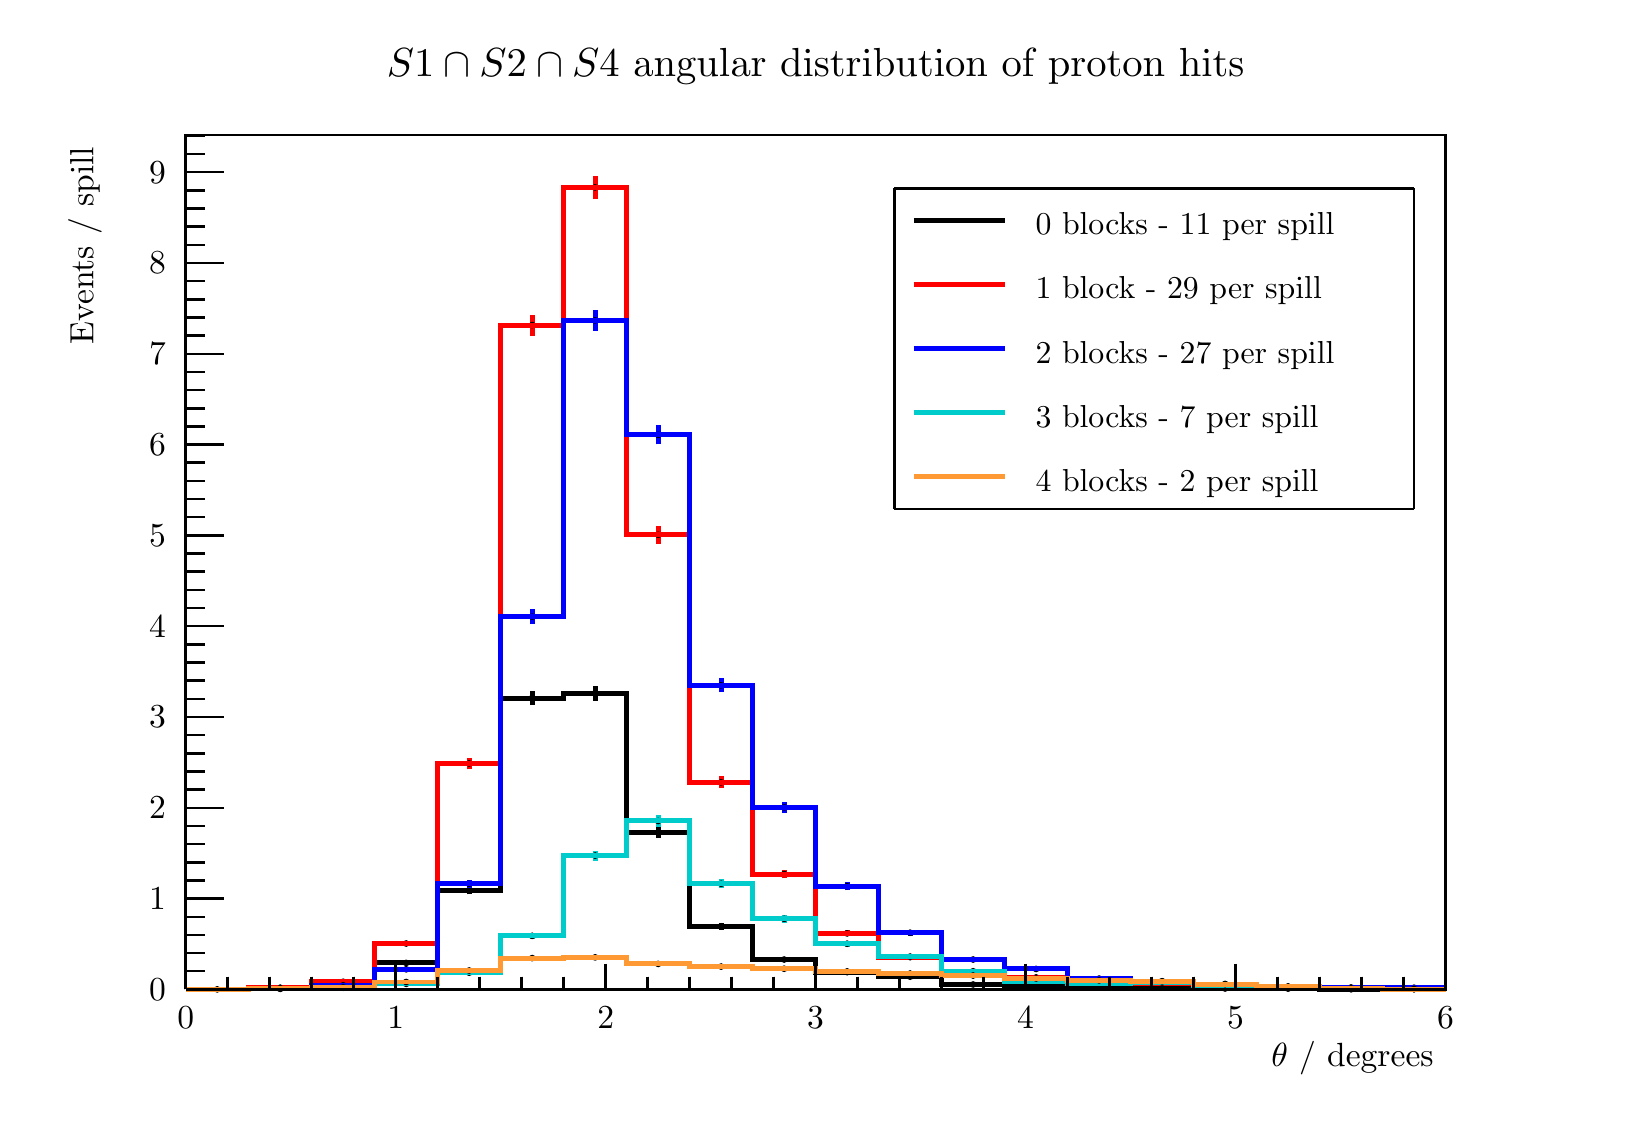
\begin{tikzpicture}
\pgfdeclareplotmark{cross} {
\pgfpathmoveto{\pgfpoint{-0.3\pgfplotmarksize}{\pgfplotmarksize}}
\pgfpathlineto{\pgfpoint{+0.3\pgfplotmarksize}{\pgfplotmarksize}}
\pgfpathlineto{\pgfpoint{+0.3\pgfplotmarksize}{0.3\pgfplotmarksize}}
\pgfpathlineto{\pgfpoint{+1\pgfplotmarksize}{0.3\pgfplotmarksize}}
\pgfpathlineto{\pgfpoint{+1\pgfplotmarksize}{-0.3\pgfplotmarksize}}
\pgfpathlineto{\pgfpoint{+0.3\pgfplotmarksize}{-0.3\pgfplotmarksize}}
\pgfpathlineto{\pgfpoint{+0.3\pgfplotmarksize}{-1.\pgfplotmarksize}}
\pgfpathlineto{\pgfpoint{-0.3\pgfplotmarksize}{-1.\pgfplotmarksize}}
\pgfpathlineto{\pgfpoint{-0.3\pgfplotmarksize}{-0.3\pgfplotmarksize}}
\pgfpathlineto{\pgfpoint{-1.\pgfplotmarksize}{-0.3\pgfplotmarksize}}
\pgfpathlineto{\pgfpoint{-1.\pgfplotmarksize}{0.3\pgfplotmarksize}}
\pgfpathlineto{\pgfpoint{-0.3\pgfplotmarksize}{0.3\pgfplotmarksize}}
\pgfpathclose
\pgfusepathqstroke
}
\pgfdeclareplotmark{cross*} {
\pgfpathmoveto{\pgfpoint{-0.3\pgfplotmarksize}{\pgfplotmarksize}}
\pgfpathlineto{\pgfpoint{+0.3\pgfplotmarksize}{\pgfplotmarksize}}
\pgfpathlineto{\pgfpoint{+0.3\pgfplotmarksize}{0.3\pgfplotmarksize}}
\pgfpathlineto{\pgfpoint{+1\pgfplotmarksize}{0.3\pgfplotmarksize}}
\pgfpathlineto{\pgfpoint{+1\pgfplotmarksize}{-0.3\pgfplotmarksize}}
\pgfpathlineto{\pgfpoint{+0.3\pgfplotmarksize}{-0.3\pgfplotmarksize}}
\pgfpathlineto{\pgfpoint{+0.3\pgfplotmarksize}{-1.\pgfplotmarksize}}
\pgfpathlineto{\pgfpoint{-0.3\pgfplotmarksize}{-1.\pgfplotmarksize}}
\pgfpathlineto{\pgfpoint{-0.3\pgfplotmarksize}{-0.3\pgfplotmarksize}}
\pgfpathlineto{\pgfpoint{-1.\pgfplotmarksize}{-0.3\pgfplotmarksize}}
\pgfpathlineto{\pgfpoint{-1.\pgfplotmarksize}{0.3\pgfplotmarksize}}
\pgfpathlineto{\pgfpoint{-0.3\pgfplotmarksize}{0.3\pgfplotmarksize}}
\pgfpathclose
\pgfusepathqfillstroke
}
\pgfdeclareplotmark{newstar} {
\pgfpathmoveto{\pgfqpoint{0pt}{\pgfplotmarksize}}
\pgfpathlineto{\pgfqpointpolar{44}{0.5\pgfplotmarksize}}
\pgfpathlineto{\pgfqpointpolar{18}{\pgfplotmarksize}}
\pgfpathlineto{\pgfqpointpolar{-20}{0.5\pgfplotmarksize}}
\pgfpathlineto{\pgfqpointpolar{-54}{\pgfplotmarksize}}
\pgfpathlineto{\pgfqpointpolar{-90}{0.5\pgfplotmarksize}}
\pgfpathlineto{\pgfqpointpolar{234}{\pgfplotmarksize}}
\pgfpathlineto{\pgfqpointpolar{198}{0.5\pgfplotmarksize}}
\pgfpathlineto{\pgfqpointpolar{162}{\pgfplotmarksize}}
\pgfpathlineto{\pgfqpointpolar{134}{0.5\pgfplotmarksize}}
\pgfpathclose
\pgfusepathqstroke
}
\pgfdeclareplotmark{newstar*} {
\pgfpathmoveto{\pgfqpoint{0pt}{\pgfplotmarksize}}
\pgfpathlineto{\pgfqpointpolar{44}{0.5\pgfplotmarksize}}
\pgfpathlineto{\pgfqpointpolar{18}{\pgfplotmarksize}}
\pgfpathlineto{\pgfqpointpolar{-20}{0.5\pgfplotmarksize}}
\pgfpathlineto{\pgfqpointpolar{-54}{\pgfplotmarksize}}
\pgfpathlineto{\pgfqpointpolar{-90}{0.5\pgfplotmarksize}}
\pgfpathlineto{\pgfqpointpolar{234}{\pgfplotmarksize}}
\pgfpathlineto{\pgfqpointpolar{198}{0.5\pgfplotmarksize}}
\pgfpathlineto{\pgfqpointpolar{162}{\pgfplotmarksize}}
\pgfpathlineto{\pgfqpointpolar{134}{0.5\pgfplotmarksize}}
\pgfpathclose
\pgfusepathqfillstroke
}
\definecolor{c}{rgb}{1,1,1};
\draw [color=c, fill=c] (0,0) rectangle (20,13.5632);
\draw [color=c, fill=c] (2,1.35632) rectangle (18,12.2069);
\definecolor{c}{rgb}{0,0,0};
\draw [c,line width=0.9] (2,1.35632) -- (2,12.2069) -- (18,12.2069) -- (18,1.35632) -- (2,1.35632);
\definecolor{c}{rgb}{1,1,1};
\draw [color=c, fill=c] (2,1.35632) rectangle (18,12.2069);
\definecolor{c}{rgb}{0,0,0};
\draw [c,line width=0.9] (2,1.35632) -- (2,12.2069) -- (18,12.2069) -- (18,1.35632) -- (2,1.35632);
\definecolor{c}{rgb}{0,0,0.6};
\draw [c,line width=0.9] (2,1.35632) -- (2.8,1.35632) -- (2.8,1.35632) -- (3.6,1.35632) -- (3.6,1.35632) -- (4.4,1.35632) -- (4.4,1.35632) -- (5.2,1.35632) -- (5.2,1.35632) -- (6,1.35632) -- (6,1.35632) -- (6.8,1.35632) -- (6.8,1.35632) --
 (7.6,1.35632) -- (7.6,1.35632) -- (8.4,1.35632) -- (8.4,1.35632) -- (9.2,1.35632) -- (9.2,1.35632) -- (10,1.35632) -- (10,1.35632) -- (10.8,1.35632) -- (10.8,1.35632) -- (11.6,1.35632) -- (11.6,1.35632) -- (12.4,1.35632) -- (12.4,1.35632) --
 (13.2,1.35632) -- (13.2,1.35632) -- (14,1.35632) -- (14,1.35632) -- (14.8,1.35632) -- (14.8,1.35632) -- (15.6,1.35632) -- (15.6,1.35632) -- (16.4,1.35632) -- (16.4,1.35632) -- (17.2,1.35632) -- (17.2,1.35632) -- (18,1.35632);
\definecolor{c}{rgb}{0,0,0};
\draw [c,line width=0.9] (2,1.35632) -- (18,1.35632);
\draw [anchor= east] (18,0.488276) node[scale=1.2126, color=c, rotate=0]{$\theta$ / degrees};
\draw [c,line width=0.9] (2,1.68184) -- (2,1.35632);
\draw [c,line width=0.9] (2.53333,1.51908) -- (2.53333,1.35632);
\draw [c,line width=0.9] (3.06667,1.51908) -- (3.06667,1.35632);
\draw [c,line width=0.9] (3.6,1.51908) -- (3.6,1.35632);
\draw [c,line width=0.9] (4.13333,1.51908) -- (4.13333,1.35632);
\draw [c,line width=0.9] (4.66667,1.68184) -- (4.66667,1.35632);
\draw [c,line width=0.9] (5.2,1.51908) -- (5.2,1.35632);
\draw [c,line width=0.9] (5.73333,1.51908) -- (5.73333,1.35632);
\draw [c,line width=0.9] (6.26667,1.51908) -- (6.26667,1.35632);
\draw [c,line width=0.9] (6.8,1.51908) -- (6.8,1.35632);
\draw [c,line width=0.9] (7.33333,1.68184) -- (7.33333,1.35632);
\draw [c,line width=0.9] (7.86667,1.51908) -- (7.86667,1.35632);
\draw [c,line width=0.9] (8.4,1.51908) -- (8.4,1.35632);
\draw [c,line width=0.9] (8.93333,1.51908) -- (8.93333,1.35632);
\draw [c,line width=0.9] (9.46667,1.51908) -- (9.46667,1.35632);
\draw [c,line width=0.9] (10,1.68184) -- (10,1.35632);
\draw [c,line width=0.9] (10.5333,1.51908) -- (10.5333,1.35632);
\draw [c,line width=0.9] (11.0667,1.51908) -- (11.0667,1.35632);
\draw [c,line width=0.9] (11.6,1.51908) -- (11.6,1.35632);
\draw [c,line width=0.9] (12.1333,1.51908) -- (12.1333,1.35632);
\draw [c,line width=0.9] (12.6667,1.68184) -- (12.6667,1.35632);
\draw [c,line width=0.9] (13.2,1.51908) -- (13.2,1.35632);
\draw [c,line width=0.9] (13.7333,1.51908) -- (13.7333,1.35632);
\draw [c,line width=0.9] (14.2667,1.51908) -- (14.2667,1.35632);
\draw [c,line width=0.9] (14.8,1.51908) -- (14.8,1.35632);
\draw [c,line width=0.9] (15.3333,1.68184) -- (15.3333,1.35632);
\draw [c,line width=0.9] (15.8667,1.51908) -- (15.8667,1.35632);
\draw [c,line width=0.9] (16.4,1.51908) -- (16.4,1.35632);
\draw [c,line width=0.9] (16.9333,1.51908) -- (16.9333,1.35632);
\draw [c,line width=0.9] (17.4667,1.51908) -- (17.4667,1.35632);
\draw [c,line width=0.9] (18,1.68184) -- (18,1.35632);
\draw [anchor=base] (2,0.854483) node[scale=1.2126, color=c, rotate=0]{0};
\draw [anchor=base] (4.66667,0.854483) node[scale=1.2126, color=c, rotate=0]{1};
\draw [anchor=base] (7.33333,0.854483) node[scale=1.2126, color=c, rotate=0]{2};
\draw [anchor=base] (10,0.854483) node[scale=1.2126, color=c, rotate=0]{3};
\draw [anchor=base] (12.6667,0.854483) node[scale=1.2126, color=c, rotate=0]{4};
\draw [anchor=base] (15.3333,0.854483) node[scale=1.2126, color=c, rotate=0]{5};
\draw [anchor=base] (18,0.854483) node[scale=1.2126, color=c, rotate=0]{6};
\draw [c,line width=0.9] (2,1.35632) -- (2,12.2069);
\draw [anchor= east] (0.72,12.2069) node[scale=1.2126, color=c, rotate=90]{ Events / spill};
\draw [c,line width=0.9] (2.48,1.35632) -- (2,1.35632);
\draw [c,line width=0.9] (2.24,1.58696) -- (2,1.58696);
\draw [c,line width=0.9] (2.24,1.81759) -- (2,1.81759);
\draw [c,line width=0.9] (2.24,2.04823) -- (2,2.04823);
\draw [c,line width=0.9] (2.24,2.27886) -- (2,2.27886);
\draw [c,line width=0.9] (2.48,2.5095) -- (2,2.5095);
\draw [c,line width=0.9] (2.24,2.74013) -- (2,2.74013);
\draw [c,line width=0.9] (2.24,2.97077) -- (2,2.97077);
\draw [c,line width=0.9] (2.24,3.20141) -- (2,3.20141);
\draw [c,line width=0.9] (2.24,3.43204) -- (2,3.43204);
\draw [c,line width=0.9] (2.48,3.66268) -- (2,3.66268);
\draw [c,line width=0.9] (2.24,3.89331) -- (2,3.89331);
\draw [c,line width=0.9] (2.24,4.12395) -- (2,4.12395);
\draw [c,line width=0.9] (2.24,4.35458) -- (2,4.35458);
\draw [c,line width=0.9] (2.24,4.58522) -- (2,4.58522);
\draw [c,line width=0.9] (2.48,4.81585) -- (2,4.81585);
\draw [c,line width=0.9] (2.24,5.04649) -- (2,5.04649);
\draw [c,line width=0.9] (2.24,5.27712) -- (2,5.27712);
\draw [c,line width=0.9] (2.24,5.50776) -- (2,5.50776);
\draw [c,line width=0.9] (2.24,5.7384) -- (2,5.7384);
\draw [c,line width=0.9] (2.48,5.96903) -- (2,5.96903);
\draw [c,line width=0.9] (2.24,6.19967) -- (2,6.19967);
\draw [c,line width=0.9] (2.24,6.4303) -- (2,6.4303);
\draw [c,line width=0.9] (2.24,6.66094) -- (2,6.66094);
\draw [c,line width=0.9] (2.24,6.89157) -- (2,6.89157);
\draw [c,line width=0.9] (2.48,7.12221) -- (2,7.12221);
\draw [c,line width=0.9] (2.24,7.35284) -- (2,7.35284);
\draw [c,line width=0.9] (2.24,7.58348) -- (2,7.58348);
\draw [c,line width=0.9] (2.24,7.81412) -- (2,7.81412);
\draw [c,line width=0.9] (2.24,8.04475) -- (2,8.04475);
\draw [c,line width=0.9] (2.48,8.27539) -- (2,8.27539);
\draw [c,line width=0.9] (2.24,8.50602) -- (2,8.50602);
\draw [c,line width=0.9] (2.24,8.73666) -- (2,8.73666);
\draw [c,line width=0.9] (2.24,8.96729) -- (2,8.96729);
\draw [c,line width=0.9] (2.24,9.19793) -- (2,9.19793);
\draw [c,line width=0.9] (2.48,9.42856) -- (2,9.42856);
\draw [c,line width=0.9] (2.24,9.6592) -- (2,9.6592);
\draw [c,line width=0.9] (2.24,9.88983) -- (2,9.88983);
\draw [c,line width=0.9] (2.24,10.1205) -- (2,10.1205);
\draw [c,line width=0.9] (2.24,10.3511) -- (2,10.3511);
\draw [c,line width=0.9] (2.48,10.5817) -- (2,10.5817);
\draw [c,line width=0.9] (2.24,10.8124) -- (2,10.8124);
\draw [c,line width=0.9] (2.24,11.043) -- (2,11.043);
\draw [c,line width=0.9] (2.24,11.2736) -- (2,11.2736);
\draw [c,line width=0.9] (2.24,11.5043) -- (2,11.5043);
\draw [c,line width=0.9] (2.48,11.7349) -- (2,11.7349);
\draw [c,line width=0.9] (2.48,11.7349) -- (2,11.7349);
\draw [c,line width=0.9] (2.24,11.9656) -- (2,11.9656);
\draw [c,line width=0.9] (2.24,12.1962) -- (2,12.1962);
\draw [anchor= east] (1.9,1.35632) node[scale=1.2126, color=c, rotate=0]{0};
\draw [anchor= east] (1.9,2.5095) node[scale=1.2126, color=c, rotate=0]{1};
\draw [anchor= east] (1.9,3.66268) node[scale=1.2126, color=c, rotate=0]{2};
\draw [anchor= east] (1.9,4.81585) node[scale=1.2126, color=c, rotate=0]{3};
\draw [anchor= east] (1.9,5.96903) node[scale=1.2126, color=c, rotate=0]{4};
\draw [anchor= east] (1.9,7.12221) node[scale=1.2126, color=c, rotate=0]{5};
\draw [anchor= east] (1.9,8.27539) node[scale=1.2126, color=c, rotate=0]{6};
\draw [anchor= east] (1.9,9.42856) node[scale=1.2126, color=c, rotate=0]{7};
\draw [anchor= east] (1.9,10.5817) node[scale=1.2126, color=c, rotate=0]{8};
\draw [anchor= east] (1.9,11.7349) node[scale=1.2126, color=c, rotate=0]{9};
\draw [c,line width=1.8] (3.2,1.36907) -- (3.2,1.3733);
\draw [c,line width=1.8] (3.2,1.3733) -- (3.2,1.37753);
\foreach \P in {(3.2,1.3733)}{\draw[mark options={color=c,fill=c},mark size=2.402402pt,mark=*,mark size=1pt] plot coordinates {\P};}
\draw [c,line width=1.8] (4,1.42823) -- (4,1.43742);
\draw [c,line width=1.8] (4,1.43742) -- (4,1.44661);
\foreach \P in {(4,1.43742)}{\draw[mark options={color=c,fill=c},mark size=2.402402pt,mark=*,mark size=1pt] plot coordinates {\P};}
\draw [c,line width=1.8] (4.8,1.67212) -- (4.8,1.6928);
\draw [c,line width=1.8] (4.8,1.6928) -- (4.8,1.71347);
\foreach \P in {(4.8,1.6928)}{\draw[mark options={color=c,fill=c},mark size=2.402402pt,mark=*,mark size=1pt] plot coordinates {\P};}
\draw [c,line width=1.8] (5.6,2.56355) -- (5.6,2.61121);
\draw [c,line width=1.8] (5.6,2.61121) -- (5.6,2.65886);
\foreach \P in {(5.6,2.61121)}{\draw[mark options={color=c,fill=c},mark size=2.402402pt,mark=*,mark size=1pt] plot coordinates {\P};}
\draw [c,line width=1.8] (6.4,4.96678) -- (6.4,5.05684);
\draw [c,line width=1.8] (6.4,5.05684) -- (6.4,5.14691);
\foreach \P in {(6.4,5.05684)}{\draw[mark options={color=c,fill=c},mark size=2.402402pt,mark=*,mark size=1pt] plot coordinates {\P};}
\draw [c,line width=1.8] (7.2,5.02241) -- (7.2,5.11701);
\draw [c,line width=1.8] (7.2,5.11701) -- (7.2,5.2116);
\foreach \P in {(7.2,5.11701)}{\draw[mark options={color=c,fill=c},mark size=2.402402pt,mark=*,mark size=1pt] plot coordinates {\P};}
\draw [c,line width=1.8] (8,3.28178) -- (8,3.34989);
\draw [c,line width=1.8] (8,3.34989) -- (8,3.41799);
\foreach \P in {(8,3.34989)}{\draw[mark options={color=c,fill=c},mark size=2.402402pt,mark=*,mark size=1pt] plot coordinates {\P};}
\draw [c,line width=1.8] (8.8,2.11628) -- (8.8,2.15828);
\draw [c,line width=1.8] (8.8,2.15828) -- (8.8,2.20028);
\foreach \P in {(8.8,2.15828)}{\draw[mark options={color=c,fill=c},mark size=2.402402pt,mark=*,mark size=1pt] plot coordinates {\P};}
\draw [c,line width=1.8] (9.6,1.70615) -- (9.6,1.7356);
\draw [c,line width=1.8] (9.6,1.7356) -- (9.6,1.76505);
\foreach \P in {(9.6,1.7356)}{\draw[mark options={color=c,fill=c},mark size=2.402402pt,mark=*,mark size=1pt] plot coordinates {\P};}
\draw [c,line width=1.8] (10.4,1.55295) -- (10.4,1.57505);
\draw [c,line width=1.8] (10.4,1.57505) -- (10.4,1.59714);
\foreach \P in {(10.4,1.57505)}{\draw[mark options={color=c,fill=c},mark size=2.402402pt,mark=*,mark size=1pt] plot coordinates {\P};}
\draw [c,line width=1.8] (11.2,1.49898) -- (11.2,1.51803);
\draw [c,line width=1.8] (11.2,1.51803) -- (11.2,1.53708);
\foreach \P in {(11.2,1.51803)}{\draw[mark options={color=c,fill=c},mark size=2.402402pt,mark=*,mark size=1pt] plot coordinates {\P};}
\draw [c,line width=1.8] (12,1.40758) -- (12,1.41881);
\draw [c,line width=1.8] (12,1.41881) -- (12,1.43005);
\foreach \P in {(12,1.41881)}{\draw[mark options={color=c,fill=c},mark size=2.402402pt,mark=*,mark size=1pt] plot coordinates {\P};}
\draw [c,line width=1.8] (12.8,1.39023) -- (12.8,1.39862);
\draw [c,line width=1.8] (12.8,1.39862) -- (12.8,1.40701);
\foreach \P in {(12.8,1.39862)}{\draw[mark options={color=c,fill=c},mark size=2.402402pt,mark=*,mark size=1pt] plot coordinates {\P};}
\draw [c,line width=1.8] (13.6,1.38187) -- (13.6,1.39153);
\draw [c,line width=1.8] (13.6,1.39153) -- (13.6,1.4012);
\foreach \P in {(13.6,1.39153)}{\draw[mark options={color=c,fill=c},mark size=2.402402pt,mark=*,mark size=1pt] plot coordinates {\P};}
\draw [c,line width=1.8] (14.4,1.37637) -- (14.4,1.3839);
\draw [c,line width=1.8] (14.4,1.3839) -- (14.4,1.39144);
\foreach \P in {(14.4,1.3839)}{\draw[mark options={color=c,fill=c},mark size=2.402402pt,mark=*,mark size=1pt] plot coordinates {\P};}
\draw [c,line width=1.8] (15.2,1.36247) -- (15.2,1.36751);
\draw [c,line width=1.8] (15.2,1.36751) -- (15.2,1.37255);
\foreach \P in {(15.2,1.36751)}{\draw[mark options={color=c,fill=c},mark size=2.402402pt,mark=*,mark size=1pt] plot coordinates {\P};}
\draw [c,line width=1.8] (16,1.36227) -- (16,1.366);
\draw [c,line width=1.8] (16,1.366) -- (16,1.36973);
\foreach \P in {(16,1.366)}{\draw[mark options={color=c,fill=c},mark size=2.402402pt,mark=*,mark size=1pt] plot coordinates {\P};}
\draw [c,line width=1.8] (16.8,1.35632) -- (16.8,1.35796);
\draw [c,line width=1.8] (16.8,1.35796) -- (16.8,1.35961);
\foreach \P in {(16.8,1.35796)}{\draw[mark options={color=c,fill=c},mark size=2.402402pt,mark=*,mark size=1pt] plot coordinates {\P};}
\draw [c,line width=1.8] (17.6,1.35632) -- (17.6,1.36005);
\draw [c,line width=1.8] (17.6,1.36005) -- (17.6,1.36378);
\foreach \P in {(17.6,1.36005)}{\draw[mark options={color=c,fill=c},mark size=2.402402pt,mark=*,mark size=1pt] plot coordinates {\P};}
\draw [c,line width=1.8] (2,1.35632) -- (2.8,1.35632) -- (2.8,1.3733) -- (3.6,1.3733) -- (3.6,1.43742) -- (4.4,1.43742) -- (4.4,1.6928) -- (5.2,1.6928) -- (5.2,2.61121) -- (6,2.61121) -- (6,5.05684) -- (6.8,5.05684) -- (6.8,5.11701) -- (7.6,5.11701)
 -- (7.6,3.34989) -- (8.4,3.34989) -- (8.4,2.15828) -- (9.2,2.15828) -- (9.2,1.7356) -- (10,1.7356) -- (10,1.57505) -- (10.8,1.57505) -- (10.8,1.51803) -- (11.6,1.51803) -- (11.6,1.41881) -- (12.4,1.41881) -- (12.4,1.39862) -- (13.2,1.39862) --
 (13.2,1.39153) -- (14,1.39153) -- (14,1.3839) -- (14.8,1.3839) -- (14.8,1.36751) -- (15.6,1.36751) -- (15.6,1.366) -- (16.4,1.366) -- (16.4,1.35796) -- (17.2,1.35796) -- (17.2,1.36005) -- (18,1.36005);
\definecolor{c}{rgb}{1,0,0};
\draw [c,line width=1.8] (3.2,1.37162) -- (3.2,1.37796);
\draw [c,line width=1.8] (3.2,1.37796) -- (3.2,1.38429);
\definecolor{c}{rgb}{0,0,0};
\foreach \P in {(3.2,1.37796)}{\draw[mark options={color=c,fill=c},mark size=2.402402pt,mark=*,mark size=1pt] plot coordinates {\P};}
\definecolor{c}{rgb}{1,0,0};
\draw [c,line width=1.8] (4,1.44099) -- (4,1.45349);
\draw [c,line width=1.8] (4,1.45349) -- (4,1.466);
\definecolor{c}{rgb}{0,0,0};
\foreach \P in {(4,1.45349)}{\draw[mark options={color=c,fill=c},mark size=2.402402pt,mark=*,mark size=1pt] plot coordinates {\P};}
\definecolor{c}{rgb}{1,0,0};
\draw [c,line width=1.8] (4.8,1.90595) -- (4.8,1.93895);
\draw [c,line width=1.8] (4.8,1.93895) -- (4.8,1.97196);
\definecolor{c}{rgb}{0,0,0};
\foreach \P in {(4.8,1.93895)}{\draw[mark options={color=c,fill=c},mark size=2.402402pt,mark=*,mark size=1pt] plot coordinates {\P};}
\definecolor{c}{rgb}{1,0,0};
\draw [c,line width=1.8] (5.6,4.15112) -- (5.6,4.22584);
\draw [c,line width=1.8] (5.6,4.22584) -- (5.6,4.30055);
\definecolor{c}{rgb}{0,0,0};
\foreach \P in {(5.6,4.22584)}{\draw[mark options={color=c,fill=c},mark size=2.402402pt,mark=*,mark size=1pt] plot coordinates {\P};}
\definecolor{c}{rgb}{1,0,0};
\draw [c,line width=1.8] (6.4,9.65938) -- (6.4,9.79309);
\draw [c,line width=1.8] (6.4,9.79309) -- (6.4,9.92681);
\definecolor{c}{rgb}{0,0,0};
\foreach \P in {(6.4,9.79309)}{\draw[mark options={color=c,fill=c},mark size=2.402402pt,mark=*,mark size=1pt] plot coordinates {\P};}
\definecolor{c}{rgb}{1,0,0};
\draw [c,line width=1.8] (7.2,11.392) -- (7.2,11.5411);
\draw [c,line width=1.8] (7.2,11.5411) -- (7.2,11.6902);
\definecolor{c}{rgb}{0,0,0};
\foreach \P in {(7.2,11.5411)}{\draw[mark options={color=c,fill=c},mark size=2.402402pt,mark=*,mark size=1pt] plot coordinates {\P};}
\definecolor{c}{rgb}{1,0,0};
\draw [c,line width=1.8] (8,7.01779) -- (8,7.12997);
\draw [c,line width=1.8] (8,7.12997) -- (8,7.24215);
\definecolor{c}{rgb}{0,0,0};
\foreach \P in {(8,7.12997)}{\draw[mark options={color=c,fill=c},mark size=2.402402pt,mark=*,mark size=1pt] plot coordinates {\P};}
\definecolor{c}{rgb}{1,0,0};
\draw [c,line width=1.8] (8.8,3.91124) -- (8.8,3.98602);
\draw [c,line width=1.8] (8.8,3.98602) -- (8.8,4.0608);
\definecolor{c}{rgb}{0,0,0};
\foreach \P in {(8.8,3.98602)}{\draw[mark options={color=c,fill=c},mark size=2.402402pt,mark=*,mark size=1pt] plot coordinates {\P};}
\definecolor{c}{rgb}{1,0,0};
\draw [c,line width=1.8] (9.6,2.76618) -- (9.6,2.82168);
\draw [c,line width=1.8] (9.6,2.82168) -- (9.6,2.87719);
\definecolor{c}{rgb}{0,0,0};
\foreach \P in {(9.6,2.82168)}{\draw[mark options={color=c,fill=c},mark size=2.402402pt,mark=*,mark size=1pt] plot coordinates {\P};}
\definecolor{c}{rgb}{1,0,0};
\draw [c,line width=1.8] (10.4,2.02843) -- (10.4,2.06711);
\draw [c,line width=1.8] (10.4,2.06711) -- (10.4,2.1058);
\definecolor{c}{rgb}{0,0,0};
\foreach \P in {(10.4,2.06711)}{\draw[mark options={color=c,fill=c},mark size=2.402402pt,mark=*,mark size=1pt] plot coordinates {\P};}
\definecolor{c}{rgb}{1,0,0};
\draw [c,line width=1.8] (11.2,1.73628) -- (11.2,1.76561);
\draw [c,line width=1.8] (11.2,1.76561) -- (11.2,1.79495);
\definecolor{c}{rgb}{0,0,0};
\foreach \P in {(11.2,1.76561)}{\draw[mark options={color=c,fill=c},mark size=2.402402pt,mark=*,mark size=1pt] plot coordinates {\P};}
\definecolor{c}{rgb}{1,0,0};
\draw [c,line width=1.8] (12,1.5353) -- (12,1.55634);
\draw [c,line width=1.8] (12,1.55634) -- (12,1.57739);
\definecolor{c}{rgb}{0,0,0};
\foreach \P in {(12,1.55634)}{\draw[mark options={color=c,fill=c},mark size=2.402402pt,mark=*,mark size=1pt] plot coordinates {\P};}
\definecolor{c}{rgb}{1,0,0};
\draw [c,line width=1.8] (12.8,1.49073) -- (12.8,1.50855);
\draw [c,line width=1.8] (12.8,1.50855) -- (12.8,1.52638);
\definecolor{c}{rgb}{0,0,0};
\foreach \P in {(12.8,1.50855)}{\draw[mark options={color=c,fill=c},mark size=2.402402pt,mark=*,mark size=1pt] plot coordinates {\P};}
\definecolor{c}{rgb}{1,0,0};
\draw [c,line width=1.8] (13.6,1.47258) -- (13.6,1.48978);
\draw [c,line width=1.8] (13.6,1.48978) -- (13.6,1.50697);
\definecolor{c}{rgb}{0,0,0};
\foreach \P in {(13.6,1.48978)}{\draw[mark options={color=c,fill=c},mark size=2.402402pt,mark=*,mark size=1pt] plot coordinates {\P};}
\definecolor{c}{rgb}{1,0,0};
\draw [c,line width=1.8] (14.4,1.4201) -- (14.4,1.43303);
\draw [c,line width=1.8] (14.4,1.43303) -- (14.4,1.44596);
\definecolor{c}{rgb}{0,0,0};
\foreach \P in {(14.4,1.43303)}{\draw[mark options={color=c,fill=c},mark size=2.402402pt,mark=*,mark size=1pt] plot coordinates {\P};}
\definecolor{c}{rgb}{1,0,0};
\draw [c,line width=1.8] (15.2,1.38109) -- (15.2,1.389);
\draw [c,line width=1.8] (15.2,1.389) -- (15.2,1.39691);
\definecolor{c}{rgb}{0,0,0};
\foreach \P in {(15.2,1.389)}{\draw[mark options={color=c,fill=c},mark size=2.402402pt,mark=*,mark size=1pt] plot coordinates {\P};}
\definecolor{c}{rgb}{1,0,0};
\draw [c,line width=1.8] (16,1.37467) -- (16,1.38246);
\draw [c,line width=1.8] (16,1.38246) -- (16,1.39025);
\definecolor{c}{rgb}{0,0,0};
\foreach \P in {(16,1.38246)}{\draw[mark options={color=c,fill=c},mark size=2.402402pt,mark=*,mark size=1pt] plot coordinates {\P};}
\definecolor{c}{rgb}{1,0,0};
\draw [c,line width=1.8] (16.8,1.36157) -- (16.8,1.36627);
\draw [c,line width=1.8] (16.8,1.36627) -- (16.8,1.37098);
\definecolor{c}{rgb}{0,0,0};
\foreach \P in {(16.8,1.36627)}{\draw[mark options={color=c,fill=c},mark size=2.402402pt,mark=*,mark size=1pt] plot coordinates {\P};}
\definecolor{c}{rgb}{1,0,0};
\draw [c,line width=1.8] (2,1.35632) -- (2.8,1.35632) -- (2.8,1.37796) -- (3.6,1.37796) -- (3.6,1.45349) -- (4.4,1.45349) -- (4.4,1.93895) -- (5.2,1.93895) -- (5.2,4.22584) -- (6,4.22584) -- (6,9.79309) -- (6.8,9.79309) -- (6.8,11.5411) --
 (7.6,11.5411) -- (7.6,7.12997) -- (8.4,7.12997) -- (8.4,3.98602) -- (9.2,3.98602) -- (9.2,2.82168) -- (10,2.82168) -- (10,2.06711) -- (10.8,2.06711) -- (10.8,1.76561) -- (11.6,1.76561) -- (11.6,1.55634) -- (12.4,1.55634) -- (12.4,1.50855) --
 (13.2,1.50855) -- (13.2,1.48978) -- (14,1.48978) -- (14,1.43303) -- (14.8,1.43303) -- (14.8,1.389) -- (15.6,1.389) -- (15.6,1.38246) -- (16.4,1.38246) -- (16.4,1.36627) -- (17.2,1.36627) -- (17.2,1.35632) -- (18,1.35632);
\definecolor{c}{rgb}{0,0,1};
\draw [c,line width=1.8] (3.2,1.36602) -- (3.2,1.37135);
\draw [c,line width=1.8] (3.2,1.37135) -- (3.2,1.37669);
\definecolor{c}{rgb}{0,0,0};
\foreach \P in {(3.2,1.37135)}{\draw[mark options={color=c,fill=c},mark size=2.402402pt,mark=*,mark size=1pt] plot coordinates {\P};}
\definecolor{c}{rgb}{0,0,1};
\draw [c,line width=1.8] (4,1.39968) -- (4,1.40866);
\draw [c,line width=1.8] (4,1.40866) -- (4,1.41764);
\definecolor{c}{rgb}{0,0,0};
\foreach \P in {(4,1.40866)}{\draw[mark options={color=c,fill=c},mark size=2.402402pt,mark=*,mark size=1pt] plot coordinates {\P};}
\definecolor{c}{rgb}{0,0,1};
\draw [c,line width=1.8] (4.8,1.59071) -- (4.8,1.61147);
\draw [c,line width=1.8] (4.8,1.61147) -- (4.8,1.63223);
\definecolor{c}{rgb}{0,0,0};
\foreach \P in {(4.8,1.61147)}{\draw[mark options={color=c,fill=c},mark size=2.402402pt,mark=*,mark size=1pt] plot coordinates {\P};}
\definecolor{c}{rgb}{0,0,1};
\draw [c,line width=1.8] (5.6,2.64778) -- (5.6,2.69632);
\draw [c,line width=1.8] (5.6,2.69632) -- (5.6,2.74486);
\definecolor{c}{rgb}{0,0,0};
\foreach \P in {(5.6,2.69632)}{\draw[mark options={color=c,fill=c},mark size=2.402402pt,mark=*,mark size=1pt] plot coordinates {\P};}
\definecolor{c}{rgb}{0,0,1};
\draw [c,line width=1.8] (6.4,5.99525) -- (6.4,6.08958);
\draw [c,line width=1.8] (6.4,6.08958) -- (6.4,6.18392);
\definecolor{c}{rgb}{0,0,0};
\foreach \P in {(6.4,6.08958)}{\draw[mark options={color=c,fill=c},mark size=2.402402pt,mark=*,mark size=1pt] plot coordinates {\P};}
\definecolor{c}{rgb}{0,0,1};
\draw [c,line width=1.8] (7.2,9.72165) -- (7.2,9.85277);
\draw [c,line width=1.8] (7.2,9.85277) -- (7.2,9.98388);
\definecolor{c}{rgb}{0,0,0};
\foreach \P in {(7.2,9.85277)}{\draw[mark options={color=c,fill=c},mark size=2.402402pt,mark=*,mark size=1pt] plot coordinates {\P};}
\definecolor{c}{rgb}{0,0,1};
\draw [c,line width=1.8] (8,8.27773) -- (8,8.39895);
\draw [c,line width=1.8] (8,8.39895) -- (8,8.52017);
\definecolor{c}{rgb}{0,0,0};
\foreach \P in {(8,8.39895)}{\draw[mark options={color=c,fill=c},mark size=2.402402pt,mark=*,mark size=1pt] plot coordinates {\P};}
\definecolor{c}{rgb}{0,0,1};
\draw [c,line width=1.8] (8.8,5.1306) -- (8.8,5.21872);
\draw [c,line width=1.8] (8.8,5.21872) -- (8.8,5.30685);
\definecolor{c}{rgb}{0,0,0};
\foreach \P in {(8.8,5.21872)}{\draw[mark options={color=c,fill=c},mark size=2.402402pt,mark=*,mark size=1pt] plot coordinates {\P};}
\definecolor{c}{rgb}{0,0,1};
\draw [c,line width=1.8] (9.6,3.59935) -- (9.6,3.6676);
\draw [c,line width=1.8] (9.6,3.6676) -- (9.6,3.73585);
\definecolor{c}{rgb}{0,0,0};
\foreach \P in {(9.6,3.6676)}{\draw[mark options={color=c,fill=c},mark size=2.402402pt,mark=*,mark size=1pt] plot coordinates {\P};}
\definecolor{c}{rgb}{0,0,1};
\draw [c,line width=1.8] (10.4,2.61599) -- (10.4,2.66745);
\draw [c,line width=1.8] (10.4,2.66745) -- (10.4,2.71891);
\definecolor{c}{rgb}{0,0,0};
\foreach \P in {(10.4,2.66745)}{\draw[mark options={color=c,fill=c},mark size=2.402402pt,mark=*,mark size=1pt] plot coordinates {\P};}
\definecolor{c}{rgb}{0,0,1};
\draw [c,line width=1.8] (11.2,2.03802) -- (11.2,2.07642);
\draw [c,line width=1.8] (11.2,2.07642) -- (11.2,2.11483);
\definecolor{c}{rgb}{0,0,0};
\foreach \P in {(11.2,2.07642)}{\draw[mark options={color=c,fill=c},mark size=2.402402pt,mark=*,mark size=1pt] plot coordinates {\P};}
\definecolor{c}{rgb}{0,0,1};
\draw [c,line width=1.8] (12,1.70768) -- (12,1.73565);
\draw [c,line width=1.8] (12,1.73565) -- (12,1.76361);
\definecolor{c}{rgb}{0,0,0};
\foreach \P in {(12,1.73565)}{\draw[mark options={color=c,fill=c},mark size=2.402402pt,mark=*,mark size=1pt] plot coordinates {\P};}
\definecolor{c}{rgb}{0,0,1};
\draw [c,line width=1.8] (12.8,1.59297) -- (12.8,1.61596);
\draw [c,line width=1.8] (12.8,1.61596) -- (12.8,1.63896);
\definecolor{c}{rgb}{0,0,0};
\foreach \P in {(12.8,1.61596)}{\draw[mark options={color=c,fill=c},mark size=2.402402pt,mark=*,mark size=1pt] plot coordinates {\P};}
\definecolor{c}{rgb}{0,0,1};
\draw [c,line width=1.8] (13.6,1.47604) -- (13.6,1.49308);
\draw [c,line width=1.8] (13.6,1.49308) -- (13.6,1.51011);
\definecolor{c}{rgb}{0,0,0};
\foreach \P in {(13.6,1.49308)}{\draw[mark options={color=c,fill=c},mark size=2.402402pt,mark=*,mark size=1pt] plot coordinates {\P};}
\definecolor{c}{rgb}{0,0,1};
\draw [c,line width=1.8] (14.4,1.44567) -- (14.4,1.46005);
\draw [c,line width=1.8] (14.4,1.46005) -- (14.4,1.47444);
\definecolor{c}{rgb}{0,0,0};
\foreach \P in {(14.4,1.46005)}{\draw[mark options={color=c,fill=c},mark size=2.402402pt,mark=*,mark size=1pt] plot coordinates {\P};}
\definecolor{c}{rgb}{0,0,1};
\draw [c,line width=1.8] (15.2,1.41305) -- (15.2,1.42495);
\draw [c,line width=1.8] (15.2,1.42495) -- (15.2,1.43686);
\definecolor{c}{rgb}{0,0,0};
\foreach \P in {(15.2,1.42495)}{\draw[mark options={color=c,fill=c},mark size=2.402402pt,mark=*,mark size=1pt] plot coordinates {\P};}
\definecolor{c}{rgb}{0,0,1};
\draw [c,line width=1.8] (16,1.37605) -- (16,1.38313);
\draw [c,line width=1.8] (16,1.38313) -- (16,1.39021);
\definecolor{c}{rgb}{0,0,0};
\foreach \P in {(16,1.38313)}{\draw[mark options={color=c,fill=c},mark size=2.402402pt,mark=*,mark size=1pt] plot coordinates {\P};}
\definecolor{c}{rgb}{0,0,1};
\draw [c,line width=1.8] (16.8,1.37376) -- (16.8,1.38092);
\draw [c,line width=1.8] (16.8,1.38092) -- (16.8,1.38807);
\definecolor{c}{rgb}{0,0,0};
\foreach \P in {(16.8,1.38092)}{\draw[mark options={color=c,fill=c},mark size=2.402402pt,mark=*,mark size=1pt] plot coordinates {\P};}
\definecolor{c}{rgb}{0,0,1};
\draw [c,line width=1.8] (17.6,1.37086) -- (17.6,1.37792);
\draw [c,line width=1.8] (17.6,1.37792) -- (17.6,1.38497);
\definecolor{c}{rgb}{0,0,0};
\foreach \P in {(17.6,1.37792)}{\draw[mark options={color=c,fill=c},mark size=2.402402pt,mark=*,mark size=1pt] plot coordinates {\P};}
\definecolor{c}{rgb}{0,0,1};
\draw [c,line width=1.8] (2,1.35632) -- (2.8,1.35632) -- (2.8,1.37135) -- (3.6,1.37135) -- (3.6,1.40866) -- (4.4,1.40866) -- (4.4,1.61147) -- (5.2,1.61147) -- (5.2,2.69632) -- (6,2.69632) -- (6,6.08958) -- (6.8,6.08958) -- (6.8,9.85277) --
 (7.6,9.85277) -- (7.6,8.39895) -- (8.4,8.39895) -- (8.4,5.21872) -- (9.2,5.21872) -- (9.2,3.6676) -- (10,3.6676) -- (10,2.66745) -- (10.8,2.66745) -- (10.8,2.07642) -- (11.6,2.07642) -- (11.6,1.73565) -- (12.4,1.73565) -- (12.4,1.61596) --
 (13.2,1.61596) -- (13.2,1.49308) -- (14,1.49308) -- (14,1.46005) -- (14.8,1.46005) -- (14.8,1.42495) -- (15.6,1.42495) -- (15.6,1.38313) -- (16.4,1.38313) -- (16.4,1.38092) -- (17.2,1.38092) -- (17.2,1.37792) -- (18,1.37792);
\definecolor{c}{rgb}{0,0.8,0.8};
\draw [c,line width=1.8] (3.2,1.36119) -- (3.2,1.36578);
\draw [c,line width=1.8] (3.2,1.36578) -- (3.2,1.37037);
\definecolor{c}{rgb}{0,0,0};
\foreach \P in {(3.2,1.36578)}{\draw[mark options={color=c,fill=c},mark size=2.402402pt,mark=*,mark size=1pt] plot coordinates {\P};}
\definecolor{c}{rgb}{0,0.8,0.8};
\draw [c,line width=1.8] (4,1.37046) -- (4,1.37758);
\draw [c,line width=1.8] (4,1.37758) -- (4,1.3847);
\definecolor{c}{rgb}{0,0,0};
\foreach \P in {(4,1.37758)}{\draw[mark options={color=c,fill=c},mark size=2.402402pt,mark=*,mark size=1pt] plot coordinates {\P};}
\definecolor{c}{rgb}{0,0.8,0.8};
\draw [c,line width=1.8] (4.8,1.41388) -- (4.8,1.42652);
\draw [c,line width=1.8] (4.8,1.42652) -- (4.8,1.43915);
\definecolor{c}{rgb}{0,0,0};
\foreach \P in {(4.8,1.42652)}{\draw[mark options={color=c,fill=c},mark size=2.402402pt,mark=*,mark size=1pt] plot coordinates {\P};}
\definecolor{c}{rgb}{0,0.8,0.8};
\draw [c,line width=1.8] (5.6,1.54618) -- (5.6,1.5683);
\draw [c,line width=1.8] (5.6,1.5683) -- (5.6,1.59042);
\definecolor{c}{rgb}{0,0,0};
\foreach \P in {(5.6,1.5683)}{\draw[mark options={color=c,fill=c},mark size=2.402402pt,mark=*,mark size=1pt] plot coordinates {\P};}
\definecolor{c}{rgb}{0,0.8,0.8};
\draw [c,line width=1.8] (6.4,1.99746) -- (6.4,2.03657);
\draw [c,line width=1.8] (6.4,2.03657) -- (6.4,2.07567);
\definecolor{c}{rgb}{0,0,0};
\foreach \P in {(6.4,2.03657)}{\draw[mark options={color=c,fill=c},mark size=2.402402pt,mark=*,mark size=1pt] plot coordinates {\P};}
\definecolor{c}{rgb}{0,0.8,0.8};
\draw [c,line width=1.8] (7.2,2.99164) -- (7.2,3.05593);
\draw [c,line width=1.8] (7.2,3.05593) -- (7.2,3.12021);
\definecolor{c}{rgb}{0,0,0};
\foreach \P in {(7.2,3.05593)}{\draw[mark options={color=c,fill=c},mark size=2.402402pt,mark=*,mark size=1pt] plot coordinates {\P};}
\definecolor{c}{rgb}{0,0.8,0.8};
\draw [c,line width=1.8] (8,3.42171) -- (8,3.49548);
\draw [c,line width=1.8] (8,3.49548) -- (8,3.56925);
\definecolor{c}{rgb}{0,0,0};
\foreach \P in {(8,3.49548)}{\draw[mark options={color=c,fill=c},mark size=2.402402pt,mark=*,mark size=1pt] plot coordinates {\P};}
\definecolor{c}{rgb}{0,0.8,0.8};
\draw [c,line width=1.8] (8.8,2.63928) -- (8.8,2.69729);
\draw [c,line width=1.8] (8.8,2.69729) -- (8.8,2.75529);
\definecolor{c}{rgb}{0,0,0};
\foreach \P in {(8.8,2.69729)}{\draw[mark options={color=c,fill=c},mark size=2.402402pt,mark=*,mark size=1pt] plot coordinates {\P};}
\definecolor{c}{rgb}{0,0.8,0.8};
\draw [c,line width=1.8] (9.6,2.20541) -- (9.6,2.25207);
\draw [c,line width=1.8] (9.6,2.25207) -- (9.6,2.29874);
\definecolor{c}{rgb}{0,0,0};
\foreach \P in {(9.6,2.25207)}{\draw[mark options={color=c,fill=c},mark size=2.402402pt,mark=*,mark size=1pt] plot coordinates {\P};}
\definecolor{c}{rgb}{0,0.8,0.8};
\draw [c,line width=1.8] (10.4,1.89835) -- (10.4,1.93659);
\draw [c,line width=1.8] (10.4,1.93659) -- (10.4,1.97482);
\definecolor{c}{rgb}{0,0,0};
\foreach \P in {(10.4,1.93659)}{\draw[mark options={color=c,fill=c},mark size=2.402402pt,mark=*,mark size=1pt] plot coordinates {\P};}
\definecolor{c}{rgb}{0,0.8,0.8};
\draw [c,line width=1.8] (11.2,1.74069) -- (11.2,1.7732);
\draw [c,line width=1.8] (11.2,1.7732) -- (11.2,1.80571);
\definecolor{c}{rgb}{0,0,0};
\foreach \P in {(11.2,1.7732)}{\draw[mark options={color=c,fill=c},mark size=2.402402pt,mark=*,mark size=1pt] plot coordinates {\P};}
\definecolor{c}{rgb}{0,0.8,0.8};
\draw [c,line width=1.8] (12,1.56205) -- (12,1.58658);
\draw [c,line width=1.8] (12,1.58658) -- (12,1.61111);
\definecolor{c}{rgb}{0,0,0};
\foreach \P in {(12,1.58658)}{\draw[mark options={color=c,fill=c},mark size=2.402402pt,mark=*,mark size=1pt] plot coordinates {\P};}
\definecolor{c}{rgb}{0,0.8,0.8};
\draw [c,line width=1.8] (12.8,1.44034) -- (12.8,1.45586);
\draw [c,line width=1.8] (12.8,1.45586) -- (12.8,1.47138);
\definecolor{c}{rgb}{0,0,0};
\foreach \P in {(12.8,1.45586)}{\draw[mark options={color=c,fill=c},mark size=2.402402pt,mark=*,mark size=1pt] plot coordinates {\P};}
\definecolor{c}{rgb}{0,0.8,0.8};
\draw [c,line width=1.8] (13.6,1.42221) -- (13.6,1.43717);
\draw [c,line width=1.8] (13.6,1.43717) -- (13.6,1.45214);
\definecolor{c}{rgb}{0,0,0};
\foreach \P in {(13.6,1.43717)}{\draw[mark options={color=c,fill=c},mark size=2.402402pt,mark=*,mark size=1pt] plot coordinates {\P};}
\definecolor{c}{rgb}{0,0.8,0.8};
\draw [c,line width=1.8] (14.4,1.42785) -- (14.4,1.44282);
\draw [c,line width=1.8] (14.4,1.44282) -- (14.4,1.45779);
\definecolor{c}{rgb}{0,0,0};
\foreach \P in {(14.4,1.44282)}{\draw[mark options={color=c,fill=c},mark size=2.402402pt,mark=*,mark size=1pt] plot coordinates {\P};}
\definecolor{c}{rgb}{0,0.8,0.8};
\draw [c,line width=1.8] (15.2,1.38712) -- (15.2,1.39734);
\draw [c,line width=1.8] (15.2,1.39734) -- (15.2,1.40757);
\definecolor{c}{rgb}{0,0,0};
\foreach \P in {(15.2,1.39734)}{\draw[mark options={color=c,fill=c},mark size=2.402402pt,mark=*,mark size=1pt] plot coordinates {\P};}
\definecolor{c}{rgb}{0,0.8,0.8};
\draw [c,line width=1.8] (16,1.38189) -- (16,1.39167);
\draw [c,line width=1.8] (16,1.39167) -- (16,1.40145);
\definecolor{c}{rgb}{0,0,0};
\foreach \P in {(16,1.39167)}{\draw[mark options={color=c,fill=c},mark size=2.402402pt,mark=*,mark size=1pt] plot coordinates {\P};}
\definecolor{c}{rgb}{0,0.8,0.8};
\draw [c,line width=1.8] (16.8,1.35923) -- (16.8,1.36352);
\draw [c,line width=1.8] (16.8,1.36352) -- (16.8,1.3678);
\definecolor{c}{rgb}{0,0,0};
\foreach \P in {(16.8,1.36352)}{\draw[mark options={color=c,fill=c},mark size=2.402402pt,mark=*,mark size=1pt] plot coordinates {\P};}
\definecolor{c}{rgb}{0,0.8,0.8};
\draw [c,line width=1.8] (17.6,1.35756) -- (17.6,1.36105);
\draw [c,line width=1.8] (17.6,1.36105) -- (17.6,1.36454);
\definecolor{c}{rgb}{0,0,0};
\foreach \P in {(17.6,1.36105)}{\draw[mark options={color=c,fill=c},mark size=2.402402pt,mark=*,mark size=1pt] plot coordinates {\P};}
\definecolor{c}{rgb}{0,0.8,0.8};
\draw [c,line width=1.8] (2,1.35632) -- (2.8,1.35632) -- (2.8,1.36578) -- (3.6,1.36578) -- (3.6,1.37758) -- (4.4,1.37758) -- (4.4,1.42652) -- (5.2,1.42652) -- (5.2,1.5683) -- (6,1.5683) -- (6,2.03657) -- (6.8,2.03657) -- (6.8,3.05593) --
 (7.6,3.05593) -- (7.6,3.49548) -- (8.4,3.49548) -- (8.4,2.69729) -- (9.2,2.69729) -- (9.2,2.25207) -- (10,2.25207) -- (10,1.93659) -- (10.8,1.93659) -- (10.8,1.7732) -- (11.6,1.7732) -- (11.6,1.58658) -- (12.4,1.58658) -- (12.4,1.45586) --
 (13.2,1.45586) -- (13.2,1.43717) -- (14,1.43717) -- (14,1.44282) -- (14.8,1.44282) -- (14.8,1.39734) -- (15.6,1.39734) -- (15.6,1.39167) -- (16.4,1.39167) -- (16.4,1.36352) -- (17.2,1.36352) -- (17.2,1.36105) -- (18,1.36105);
\definecolor{c}{rgb}{1,0.6,0.2};
\draw [c,line width=1.8] (2.4,1.35632) -- (2.4,1.35649);
\draw [c,line width=1.8] (2.4,1.35649) -- (2.4,1.35665);
\definecolor{c}{rgb}{0,0,0};
\foreach \P in {(2.4,1.35649)}{\draw[mark options={color=c,fill=c},mark size=2.402402pt,mark=*,mark size=1pt] plot coordinates {\P};}
\definecolor{c}{rgb}{1,0.6,0.2};
\draw [c,line width=1.8] (3.2,1.36192) -- (3.2,1.36289);
\draw [c,line width=1.8] (3.2,1.36289) -- (3.2,1.36385);
\definecolor{c}{rgb}{0,0,0};
\foreach \P in {(3.2,1.36289)}{\draw[mark options={color=c,fill=c},mark size=2.402402pt,mark=*,mark size=1pt] plot coordinates {\P};}
\definecolor{c}{rgb}{1,0.6,0.2};
\draw [c,line width=1.8] (4,1.37987) -- (4,1.38165);
\draw [c,line width=1.8] (4,1.38165) -- (4,1.38342);
\definecolor{c}{rgb}{0,0,0};
\foreach \P in {(4,1.38165)}{\draw[mark options={color=c,fill=c},mark size=2.402402pt,mark=*,mark size=1pt] plot coordinates {\P};}
\definecolor{c}{rgb}{1,0.6,0.2};
\draw [c,line width=1.8] (4.8,1.44676) -- (4.8,1.45031);
\draw [c,line width=1.8] (4.8,1.45031) -- (4.8,1.45387);
\definecolor{c}{rgb}{0,0,0};
\foreach \P in {(4.8,1.45031)}{\draw[mark options={color=c,fill=c},mark size=2.402402pt,mark=*,mark size=1pt] plot coordinates {\P};}
\definecolor{c}{rgb}{1,0.6,0.2};
\draw [c,line width=1.8] (5.6,1.59048) -- (5.6,1.59631);
\draw [c,line width=1.8] (5.6,1.59631) -- (5.6,1.60215);
\definecolor{c}{rgb}{0,0,0};
\foreach \P in {(5.6,1.59631)}{\draw[mark options={color=c,fill=c},mark size=2.402402pt,mark=*,mark size=1pt] plot coordinates {\P};}
\definecolor{c}{rgb}{1,0.6,0.2};
\draw [c,line width=1.8] (6.4,1.74617) -- (6.4,1.75387);
\draw [c,line width=1.8] (6.4,1.75387) -- (6.4,1.76157);
\definecolor{c}{rgb}{0,0,0};
\foreach \P in {(6.4,1.75387)}{\draw[mark options={color=c,fill=c},mark size=2.402402pt,mark=*,mark size=1pt] plot coordinates {\P};}
\definecolor{c}{rgb}{1,0.6,0.2};
\draw [c,line width=1.8] (7.2,1.75517) -- (7.2,1.76304);
\draw [c,line width=1.8] (7.2,1.76304) -- (7.2,1.77091);
\definecolor{c}{rgb}{0,0,0};
\foreach \P in {(7.2,1.76304)}{\draw[mark options={color=c,fill=c},mark size=2.402402pt,mark=*,mark size=1pt] plot coordinates {\P};}
\definecolor{c}{rgb}{1,0.6,0.2};
\draw [c,line width=1.8] (8,1.67328) -- (8,1.6803);
\draw [c,line width=1.8] (8,1.6803) -- (8,1.68731);
\definecolor{c}{rgb}{0,0,0};
\foreach \P in {(8,1.6803)}{\draw[mark options={color=c,fill=c},mark size=2.402402pt,mark=*,mark size=1pt] plot coordinates {\P};}
\definecolor{c}{rgb}{1,0.6,0.2};
\draw [c,line width=1.8] (8.8,1.63969) -- (8.8,1.64624);
\draw [c,line width=1.8] (8.8,1.64624) -- (8.8,1.6528);
\definecolor{c}{rgb}{0,0,0};
\foreach \P in {(8.8,1.64624)}{\draw[mark options={color=c,fill=c},mark size=2.402402pt,mark=*,mark size=1pt] plot coordinates {\P};}
\definecolor{c}{rgb}{1,0.6,0.2};
\draw [c,line width=1.8] (9.6,1.61245) -- (9.6,1.61868);
\draw [c,line width=1.8] (9.6,1.61868) -- (9.6,1.62491);
\definecolor{c}{rgb}{0,0,0};
\foreach \P in {(9.6,1.61868)}{\draw[mark options={color=c,fill=c},mark size=2.402402pt,mark=*,mark size=1pt] plot coordinates {\P};}
\definecolor{c}{rgb}{1,0.6,0.2};
\draw [c,line width=1.8] (10.4,1.57878) -- (10.4,1.58458);
\draw [c,line width=1.8] (10.4,1.58458) -- (10.4,1.59038);
\definecolor{c}{rgb}{0,0,0};
\foreach \P in {(10.4,1.58458)}{\draw[mark options={color=c,fill=c},mark size=2.402402pt,mark=*,mark size=1pt] plot coordinates {\P};}
\definecolor{c}{rgb}{1,0.6,0.2};
\draw [c,line width=1.8] (11.2,1.55196) -- (11.2,1.55741);
\draw [c,line width=1.8] (11.2,1.55741) -- (11.2,1.56285);
\definecolor{c}{rgb}{0,0,0};
\foreach \P in {(11.2,1.55741)}{\draw[mark options={color=c,fill=c},mark size=2.402402pt,mark=*,mark size=1pt] plot coordinates {\P};}
\definecolor{c}{rgb}{1,0.6,0.2};
\draw [c,line width=1.8] (12,1.52709) -- (12,1.53219);
\draw [c,line width=1.8] (12,1.53219) -- (12,1.53729);
\definecolor{c}{rgb}{0,0,0};
\foreach \P in {(12,1.53219)}{\draw[mark options={color=c,fill=c},mark size=2.402402pt,mark=*,mark size=1pt] plot coordinates {\P};}
\definecolor{c}{rgb}{1,0.6,0.2};
\draw [c,line width=1.8] (12.8,1.49061) -- (12.8,1.49509);
\draw [c,line width=1.8] (12.8,1.49509) -- (12.8,1.49958);
\definecolor{c}{rgb}{0,0,0};
\foreach \P in {(12.8,1.49509)}{\draw[mark options={color=c,fill=c},mark size=2.402402pt,mark=*,mark size=1pt] plot coordinates {\P};}
\definecolor{c}{rgb}{1,0.6,0.2};
\draw [c,line width=1.8] (13.6,1.46661) -- (13.6,1.47071);
\draw [c,line width=1.8] (13.6,1.47071) -- (13.6,1.47481);
\definecolor{c}{rgb}{0,0,0};
\foreach \P in {(13.6,1.47071)}{\draw[mark options={color=c,fill=c},mark size=2.402402pt,mark=*,mark size=1pt] plot coordinates {\P};}
\definecolor{c}{rgb}{1,0.6,0.2};
\draw [c,line width=1.8] (14.4,1.45433) -- (14.4,1.45819);
\draw [c,line width=1.8] (14.4,1.45819) -- (14.4,1.46205);
\definecolor{c}{rgb}{0,0,0};
\foreach \P in {(14.4,1.45819)}{\draw[mark options={color=c,fill=c},mark size=2.402402pt,mark=*,mark size=1pt] plot coordinates {\P};}
\definecolor{c}{rgb}{1,0.6,0.2};
\draw [c,line width=1.8] (15.2,1.41923) -- (15.2,1.42231);
\draw [c,line width=1.8] (15.2,1.42231) -- (15.2,1.42539);
\definecolor{c}{rgb}{0,0,0};
\foreach \P in {(15.2,1.42231)}{\draw[mark options={color=c,fill=c},mark size=2.402402pt,mark=*,mark size=1pt] plot coordinates {\P};}
\definecolor{c}{rgb}{1,0.6,0.2};
\draw [c,line width=1.8] (16,1.39062) -- (16,1.39291);
\draw [c,line width=1.8] (16,1.39291) -- (16,1.39519);
\definecolor{c}{rgb}{0,0,0};
\foreach \P in {(16,1.39291)}{\draw[mark options={color=c,fill=c},mark size=2.402402pt,mark=*,mark size=1pt] plot coordinates {\P};}
\definecolor{c}{rgb}{1,0.6,0.2};
\draw [c,line width=1.8] (16.8,1.36854) -- (16.8,1.3699);
\draw [c,line width=1.8] (16.8,1.3699) -- (16.8,1.37127);
\definecolor{c}{rgb}{0,0,0};
\foreach \P in {(16.8,1.3699)}{\draw[mark options={color=c,fill=c},mark size=2.402402pt,mark=*,mark size=1pt] plot coordinates {\P};}
\definecolor{c}{rgb}{1,0.6,0.2};
\draw [c,line width=1.8] (17.6,1.36031) -- (17.6,1.36113);
\draw [c,line width=1.8] (17.6,1.36113) -- (17.6,1.36196);
\definecolor{c}{rgb}{0,0,0};
\foreach \P in {(17.6,1.36113)}{\draw[mark options={color=c,fill=c},mark size=2.402402pt,mark=*,mark size=1pt] plot coordinates {\P};}
\definecolor{c}{rgb}{1,0.6,0.2};
\draw [c,line width=1.8] (2,1.35632) -- (2.8,1.35632) -- (2.8,1.36289) -- (3.6,1.36289) -- (3.6,1.38165) -- (4.4,1.38165) -- (4.4,1.45031) -- (5.2,1.45031) -- (5.2,1.59631) -- (6,1.59631) -- (6,1.75387) -- (6.8,1.75387) -- (6.8,1.76304) --
 (7.6,1.76304) -- (7.6,1.6803) -- (8.4,1.6803) -- (8.4,1.64624) -- (9.2,1.64624) -- (9.2,1.61868) -- (10,1.61868) -- (10,1.58458) -- (10.8,1.58458) -- (10.8,1.55741) -- (11.6,1.55741) -- (11.6,1.53219) -- (12.4,1.53219) -- (12.4,1.49509) --
 (13.2,1.49509) -- (13.2,1.47071) -- (14,1.47071) -- (14,1.45819) -- (14.8,1.45819) -- (14.8,1.42231) -- (15.6,1.42231) -- (15.6,1.39291) -- (16.4,1.39291) -- (16.4,1.3699) -- (17.2,1.3699) -- (17.2,1.36113) -- (18,1.36113);
\definecolor{c}{rgb}{0,0,0};
\draw [c,line width=0.9] (2,1.35632) -- (18,1.35632);
\draw [c,line width=0.9] (2,1.68184) -- (2,1.35632);
\draw [c,line width=0.9] (2.53333,1.51908) -- (2.53333,1.35632);
\draw [c,line width=0.9] (3.06667,1.51908) -- (3.06667,1.35632);
\draw [c,line width=0.9] (3.6,1.51908) -- (3.6,1.35632);
\draw [c,line width=0.9] (4.13333,1.51908) -- (4.13333,1.35632);
\draw [c,line width=0.9] (4.66667,1.68184) -- (4.66667,1.35632);
\draw [c,line width=0.9] (5.2,1.51908) -- (5.2,1.35632);
\draw [c,line width=0.9] (5.73333,1.51908) -- (5.73333,1.35632);
\draw [c,line width=0.9] (6.26667,1.51908) -- (6.26667,1.35632);
\draw [c,line width=0.9] (6.8,1.51908) -- (6.8,1.35632);
\draw [c,line width=0.9] (7.33333,1.68184) -- (7.33333,1.35632);
\draw [c,line width=0.9] (7.86667,1.51908) -- (7.86667,1.35632);
\draw [c,line width=0.9] (8.4,1.51908) -- (8.4,1.35632);
\draw [c,line width=0.9] (8.93333,1.51908) -- (8.93333,1.35632);
\draw [c,line width=0.9] (9.46667,1.51908) -- (9.46667,1.35632);
\draw [c,line width=0.9] (10,1.68184) -- (10,1.35632);
\draw [c,line width=0.9] (10.5333,1.51908) -- (10.5333,1.35632);
\draw [c,line width=0.9] (11.0667,1.51908) -- (11.0667,1.35632);
\draw [c,line width=0.9] (11.6,1.51908) -- (11.6,1.35632);
\draw [c,line width=0.9] (12.1333,1.51908) -- (12.1333,1.35632);
\draw [c,line width=0.9] (12.6667,1.68184) -- (12.6667,1.35632);
\draw [c,line width=0.9] (13.2,1.51908) -- (13.2,1.35632);
\draw [c,line width=0.9] (13.7333,1.51908) -- (13.7333,1.35632);
\draw [c,line width=0.9] (14.2667,1.51908) -- (14.2667,1.35632);
\draw [c,line width=0.9] (14.8,1.51908) -- (14.8,1.35632);
\draw [c,line width=0.9] (15.3333,1.68184) -- (15.3333,1.35632);
\draw [c,line width=0.9] (15.8667,1.51908) -- (15.8667,1.35632);
\draw [c,line width=0.9] (16.4,1.51908) -- (16.4,1.35632);
\draw [c,line width=0.9] (16.9333,1.51908) -- (16.9333,1.35632);
\draw [c,line width=0.9] (17.4667,1.51908) -- (17.4667,1.35632);
\draw [c,line width=0.9] (18,1.68184) -- (18,1.35632);
\draw [c,line width=0.9] (2,1.35632) -- (2,12.2069);
\draw [c,line width=0.9] (2.48,1.35632) -- (2,1.35632);
\draw [c,line width=0.9] (2.24,1.58696) -- (2,1.58696);
\draw [c,line width=0.9] (2.24,1.81759) -- (2,1.81759);
\draw [c,line width=0.9] (2.24,2.04823) -- (2,2.04823);
\draw [c,line width=0.9] (2.24,2.27886) -- (2,2.27886);
\draw [c,line width=0.9] (2.48,2.5095) -- (2,2.5095);
\draw [c,line width=0.9] (2.24,2.74013) -- (2,2.74013);
\draw [c,line width=0.9] (2.24,2.97077) -- (2,2.97077);
\draw [c,line width=0.9] (2.24,3.20141) -- (2,3.20141);
\draw [c,line width=0.9] (2.24,3.43204) -- (2,3.43204);
\draw [c,line width=0.9] (2.48,3.66268) -- (2,3.66268);
\draw [c,line width=0.9] (2.24,3.89331) -- (2,3.89331);
\draw [c,line width=0.9] (2.24,4.12395) -- (2,4.12395);
\draw [c,line width=0.9] (2.24,4.35458) -- (2,4.35458);
\draw [c,line width=0.9] (2.24,4.58522) -- (2,4.58522);
\draw [c,line width=0.9] (2.48,4.81585) -- (2,4.81585);
\draw [c,line width=0.9] (2.24,5.04649) -- (2,5.04649);
\draw [c,line width=0.9] (2.24,5.27712) -- (2,5.27712);
\draw [c,line width=0.9] (2.24,5.50776) -- (2,5.50776);
\draw [c,line width=0.9] (2.24,5.7384) -- (2,5.7384);
\draw [c,line width=0.9] (2.48,5.96903) -- (2,5.96903);
\draw [c,line width=0.9] (2.24,6.19967) -- (2,6.19967);
\draw [c,line width=0.9] (2.24,6.4303) -- (2,6.4303);
\draw [c,line width=0.9] (2.24,6.66094) -- (2,6.66094);
\draw [c,line width=0.9] (2.24,6.89157) -- (2,6.89157);
\draw [c,line width=0.9] (2.48,7.12221) -- (2,7.12221);
\draw [c,line width=0.9] (2.24,7.35284) -- (2,7.35284);
\draw [c,line width=0.9] (2.24,7.58348) -- (2,7.58348);
\draw [c,line width=0.9] (2.24,7.81412) -- (2,7.81412);
\draw [c,line width=0.9] (2.24,8.04475) -- (2,8.04475);
\draw [c,line width=0.9] (2.48,8.27539) -- (2,8.27539);
\draw [c,line width=0.9] (2.24,8.50602) -- (2,8.50602);
\draw [c,line width=0.9] (2.24,8.73666) -- (2,8.73666);
\draw [c,line width=0.9] (2.24,8.96729) -- (2,8.96729);
\draw [c,line width=0.9] (2.24,9.19793) -- (2,9.19793);
\draw [c,line width=0.9] (2.48,9.42856) -- (2,9.42856);
\draw [c,line width=0.9] (2.24,9.6592) -- (2,9.6592);
\draw [c,line width=0.9] (2.24,9.88983) -- (2,9.88983);
\draw [c,line width=0.9] (2.24,10.1205) -- (2,10.1205);
\draw [c,line width=0.9] (2.24,10.3511) -- (2,10.3511);
\draw [c,line width=0.9] (2.48,10.5817) -- (2,10.5817);
\draw [c,line width=0.9] (2.24,10.8124) -- (2,10.8124);
\draw [c,line width=0.9] (2.24,11.043) -- (2,11.043);
\draw [c,line width=0.9] (2.24,11.2736) -- (2,11.2736);
\draw [c,line width=0.9] (2.24,11.5043) -- (2,11.5043);
\draw [c,line width=0.9] (2.48,11.7349) -- (2,11.7349);
\draw [c,line width=0.9] (2.48,11.7349) -- (2,11.7349);
\draw [c,line width=0.9] (2.24,11.9656) -- (2,11.9656);
\draw [c,line width=0.9] (2.24,12.1962) -- (2,12.1962);
\draw (10,13.0816) node[scale=1.46788, color=c, rotate=0]{$S1 \cap S2 \cap S4$ angular distribution of proton hits};
\definecolor{c}{rgb}{1,1,1};
\draw [color=c, fill=c] (11,7.45977) rectangle (17.6,11.5287);
\definecolor{c}{rgb}{0,0,0};
\draw [c,line width=0.9] (11,7.45977) -- (17.6,7.45977);
\draw [c,line width=0.9] (17.6,7.45977) -- (17.6,11.5287);
\draw [c,line width=0.9] (17.6,11.5287) -- (11,11.5287);
\draw [c,line width=0.9] (11,11.5287) -- (11,7.45977);
\draw [anchor=base west] (12.65,10.9387) node[scale=1.14878, color=c, rotate=0]{0 blocks - 11 per spill};
\draw [c,line width=1.8] (11.2475,11.1218) -- (12.4025,11.1218);
\draw [anchor=base west] (12.65,10.1249) node[scale=1.14878, color=c, rotate=0]{1 block - 29 per spill};
\definecolor{c}{rgb}{1,0,0};
\draw [c,line width=1.8] (11.2475,10.308) -- (12.4025,10.308);
\definecolor{c}{rgb}{0,0,0};
\draw [anchor=base west] (12.65,9.31115) node[scale=1.14878, color=c, rotate=0]{2 blocks - 27 per spill};
\definecolor{c}{rgb}{0,0,1};
\draw [c,line width=1.8] (11.2475,9.49425) -- (12.4025,9.49425);
\definecolor{c}{rgb}{0,0,0};
\draw [anchor=base west] (12.65,8.49736) node[scale=1.14878, color=c, rotate=0]{3 blocks - 7 per spill};
\definecolor{c}{rgb}{0,0.8,0.8};
\draw [c,line width=1.8] (11.2475,8.68046) -- (12.4025,8.68046);
\definecolor{c}{rgb}{0,0,0};
\draw [anchor=base west] (12.65,7.68356) node[scale=1.14878, color=c, rotate=0]{4 blocks - 2 per spill};
\definecolor{c}{rgb}{1,0.6,0.2};
\draw [c,line width=1.8] (11.2475,7.86667) -- (12.4025,7.86667);
\end{tikzpicture}

	   		\end{adjustbox}
   			\caption{Distribution of hits identified in $S_{4}$ as protons as a function of the number of moderator blocks and the horizontal off-axis angle, as measured from $S_{1}$.}
   		\end{minipage} 
   	
   		%\begin{minipage}[t]{0.48\textwidth}
   		%	\centering
   		%	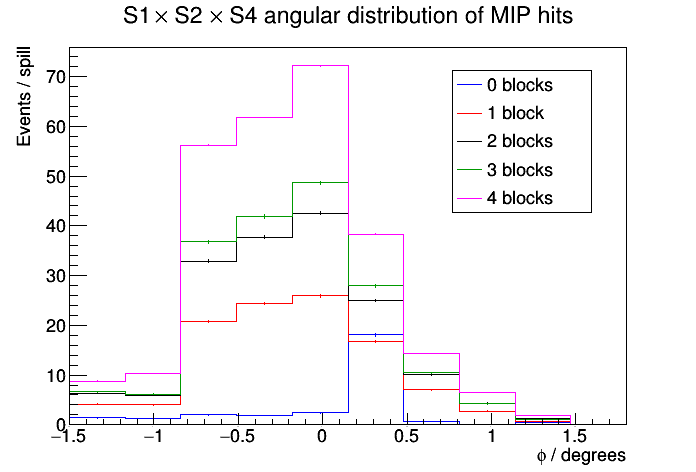
\includegraphics[width=\textwidth]{files/Figures/piS4Vert}
   		%	\caption{Distribution of hits identified in $S_{4}$ as minimum ionizing particles as a function of the number of moderator blocks and the vertical off-axis angle, as measured from $S_{1}$.}
   		%\end{minipage}
   		%\hspace{0.3cm}
   		%\begin{minipage}[t]{0.48\textwidth}
   		%	\centering
   		%	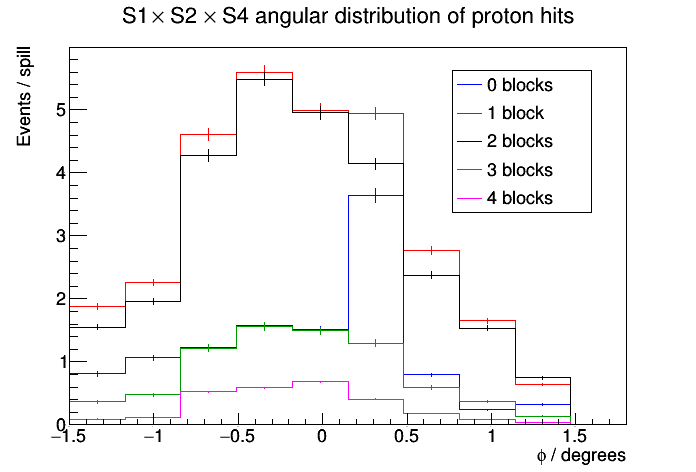
\includegraphics[width=\textwidth]{files/Figures/proS4Vert}
   		%	\caption{Distribution of hits identified in $S_{4}$ as protons as a function of the number of moderator blocks and the vertical off-axis angle, as measured from $S_{1}$.}
   		%\end{minipage}
   	
	\end{figure}	
        
   	\begin{figure}[ht]
   		\begin{minipage}[t]{0.48\textwidth}
   			\begin{adjustbox}{max totalsize={\textwidth}{.35\textheight}, center}
   				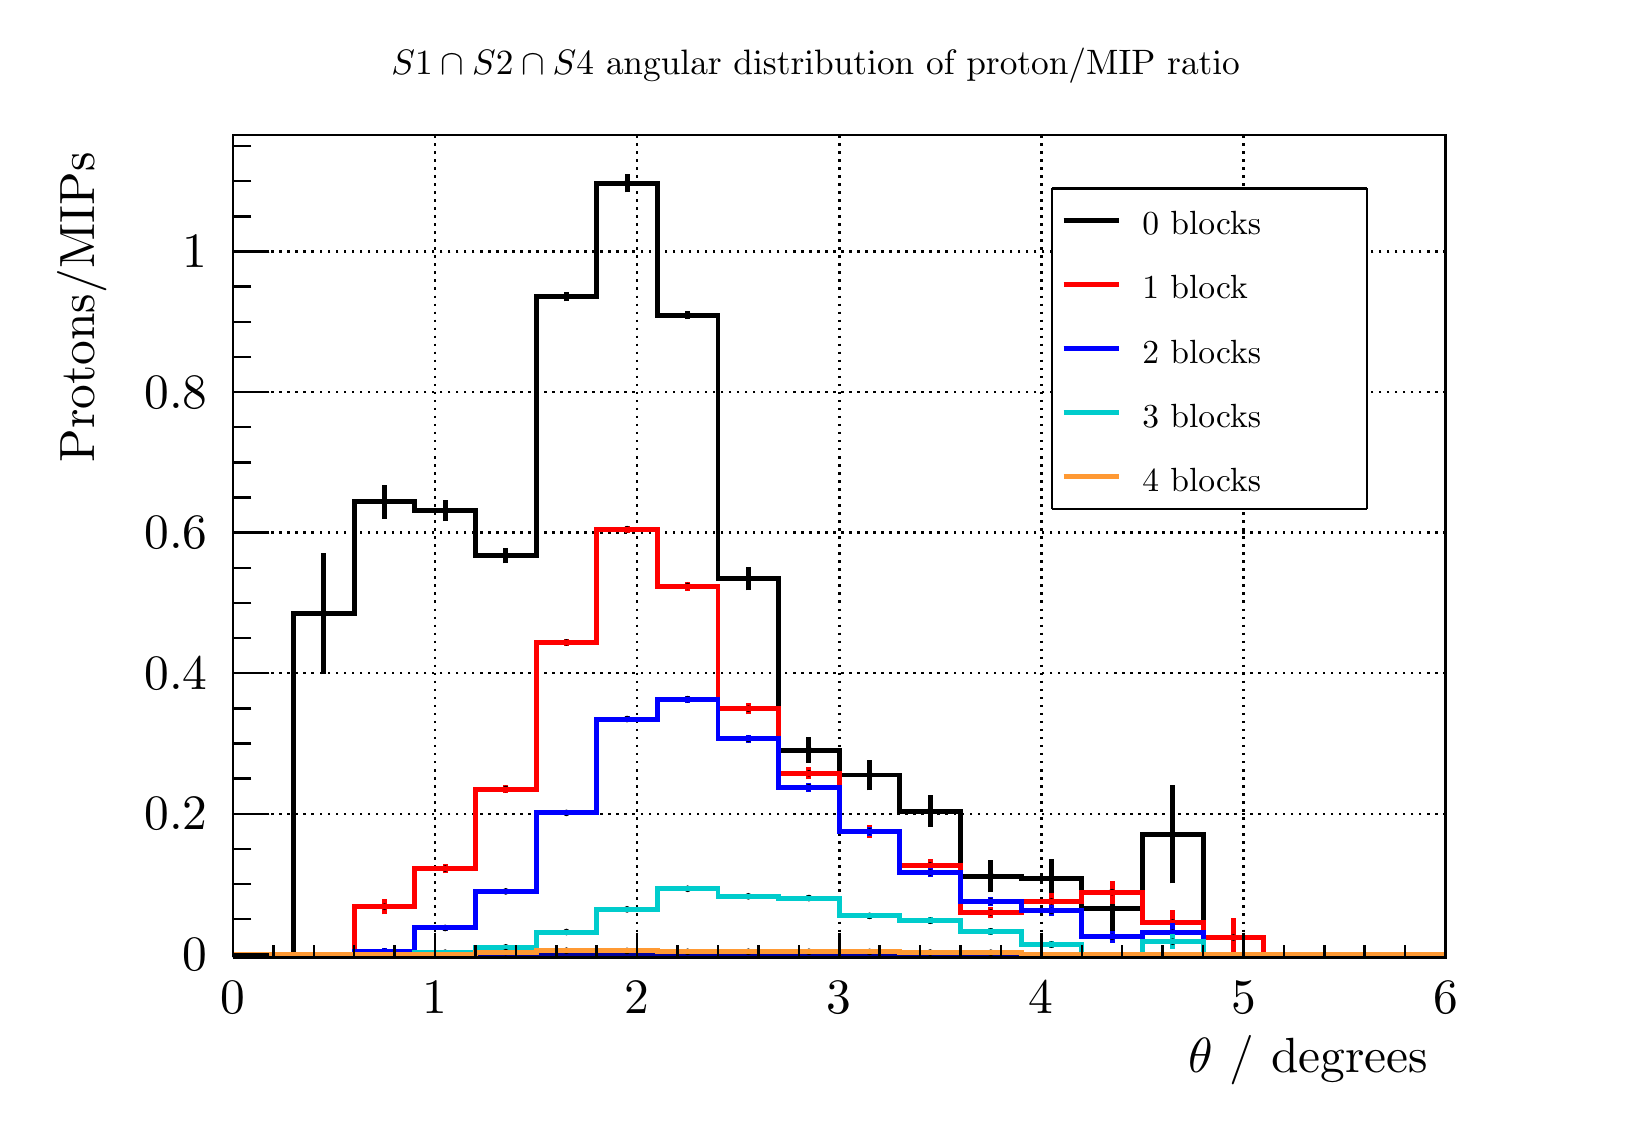
\begin{tikzpicture}
\pgfdeclareplotmark{cross} {
\pgfpathmoveto{\pgfpoint{-0.3\pgfplotmarksize}{\pgfplotmarksize}}
\pgfpathlineto{\pgfpoint{+0.3\pgfplotmarksize}{\pgfplotmarksize}}
\pgfpathlineto{\pgfpoint{+0.3\pgfplotmarksize}{0.3\pgfplotmarksize}}
\pgfpathlineto{\pgfpoint{+1\pgfplotmarksize}{0.3\pgfplotmarksize}}
\pgfpathlineto{\pgfpoint{+1\pgfplotmarksize}{-0.3\pgfplotmarksize}}
\pgfpathlineto{\pgfpoint{+0.3\pgfplotmarksize}{-0.3\pgfplotmarksize}}
\pgfpathlineto{\pgfpoint{+0.3\pgfplotmarksize}{-1.\pgfplotmarksize}}
\pgfpathlineto{\pgfpoint{-0.3\pgfplotmarksize}{-1.\pgfplotmarksize}}
\pgfpathlineto{\pgfpoint{-0.3\pgfplotmarksize}{-0.3\pgfplotmarksize}}
\pgfpathlineto{\pgfpoint{-1.\pgfplotmarksize}{-0.3\pgfplotmarksize}}
\pgfpathlineto{\pgfpoint{-1.\pgfplotmarksize}{0.3\pgfplotmarksize}}
\pgfpathlineto{\pgfpoint{-0.3\pgfplotmarksize}{0.3\pgfplotmarksize}}
\pgfpathclose
\pgfusepathqstroke
}
\pgfdeclareplotmark{cross*} {
\pgfpathmoveto{\pgfpoint{-0.3\pgfplotmarksize}{\pgfplotmarksize}}
\pgfpathlineto{\pgfpoint{+0.3\pgfplotmarksize}{\pgfplotmarksize}}
\pgfpathlineto{\pgfpoint{+0.3\pgfplotmarksize}{0.3\pgfplotmarksize}}
\pgfpathlineto{\pgfpoint{+1\pgfplotmarksize}{0.3\pgfplotmarksize}}
\pgfpathlineto{\pgfpoint{+1\pgfplotmarksize}{-0.3\pgfplotmarksize}}
\pgfpathlineto{\pgfpoint{+0.3\pgfplotmarksize}{-0.3\pgfplotmarksize}}
\pgfpathlineto{\pgfpoint{+0.3\pgfplotmarksize}{-1.\pgfplotmarksize}}
\pgfpathlineto{\pgfpoint{-0.3\pgfplotmarksize}{-1.\pgfplotmarksize}}
\pgfpathlineto{\pgfpoint{-0.3\pgfplotmarksize}{-0.3\pgfplotmarksize}}
\pgfpathlineto{\pgfpoint{-1.\pgfplotmarksize}{-0.3\pgfplotmarksize}}
\pgfpathlineto{\pgfpoint{-1.\pgfplotmarksize}{0.3\pgfplotmarksize}}
\pgfpathlineto{\pgfpoint{-0.3\pgfplotmarksize}{0.3\pgfplotmarksize}}
\pgfpathclose
\pgfusepathqfillstroke
}
\pgfdeclareplotmark{newstar} {
\pgfpathmoveto{\pgfqpoint{0pt}{\pgfplotmarksize}}
\pgfpathlineto{\pgfqpointpolar{44}{0.5\pgfplotmarksize}}
\pgfpathlineto{\pgfqpointpolar{18}{\pgfplotmarksize}}
\pgfpathlineto{\pgfqpointpolar{-20}{0.5\pgfplotmarksize}}
\pgfpathlineto{\pgfqpointpolar{-54}{\pgfplotmarksize}}
\pgfpathlineto{\pgfqpointpolar{-90}{0.5\pgfplotmarksize}}
\pgfpathlineto{\pgfqpointpolar{234}{\pgfplotmarksize}}
\pgfpathlineto{\pgfqpointpolar{198}{0.5\pgfplotmarksize}}
\pgfpathlineto{\pgfqpointpolar{162}{\pgfplotmarksize}}
\pgfpathlineto{\pgfqpointpolar{134}{0.5\pgfplotmarksize}}
\pgfpathclose
\pgfusepathqstroke
}
\pgfdeclareplotmark{newstar*} {
\pgfpathmoveto{\pgfqpoint{0pt}{\pgfplotmarksize}}
\pgfpathlineto{\pgfqpointpolar{44}{0.5\pgfplotmarksize}}
\pgfpathlineto{\pgfqpointpolar{18}{\pgfplotmarksize}}
\pgfpathlineto{\pgfqpointpolar{-20}{0.5\pgfplotmarksize}}
\pgfpathlineto{\pgfqpointpolar{-54}{\pgfplotmarksize}}
\pgfpathlineto{\pgfqpointpolar{-90}{0.5\pgfplotmarksize}}
\pgfpathlineto{\pgfqpointpolar{234}{\pgfplotmarksize}}
\pgfpathlineto{\pgfqpointpolar{198}{0.5\pgfplotmarksize}}
\pgfpathlineto{\pgfqpointpolar{162}{\pgfplotmarksize}}
\pgfpathlineto{\pgfqpointpolar{134}{0.5\pgfplotmarksize}}
\pgfpathclose
\pgfusepathqfillstroke
}
\definecolor{c}{rgb}{1,1,1};
\draw [color=c, fill=c] (0,0) rectangle (20,13.5632);
\draw [color=c, fill=c] (2.6,1.76322) rectangle (18,12.2069);
\definecolor{c}{rgb}{0,0,0};
\draw [c,line width=0.9] (2.6,1.76322) -- (2.6,12.2069) -- (18,12.2069) -- (18,1.76322) -- (2.6,1.76322);
\definecolor{c}{rgb}{1,1,1};
\draw [color=c, fill=c] (2.6,1.76322) rectangle (18,12.2069);
\definecolor{c}{rgb}{0,0,0};
\draw [c,line width=0.9] (2.6,1.76322) -- (2.6,12.2069) -- (18,12.2069) -- (18,1.76322) -- (2.6,1.76322);
\draw [c,line width=0.9] (2.6,1.76322) -- (18,1.76322);
\draw [c,dotted,line width=0.9] (2.6,12.2069) -- (2.6,1.76322);
\draw [c,dotted,line width=0.9] (5.16667,12.2069) -- (5.16667,1.76322);
\draw [c,dotted,line width=0.9] (7.73333,12.2069) -- (7.73333,1.76322);
\draw [c,dotted,line width=0.9] (10.3,12.2069) -- (10.3,1.76322);
\draw [c,dotted,line width=0.9] (12.8667,12.2069) -- (12.8667,1.76322);
\draw [c,dotted,line width=0.9] (15.4333,12.2069) -- (15.4333,1.76322);
\draw [c,dotted,line width=0.9] (18,12.2069) -- (18,1.76322);
\draw [c,line width=0.9] (2.6,1.76322) -- (2.6,12.2069);
\draw [c,dotted,line width=0.9] (18,1.80099) -- (2.6,1.80099);
\draw [c,dotted,line width=0.9] (18,3.58635) -- (2.6,3.58635);
\draw [c,dotted,line width=0.9] (18,5.37171) -- (2.6,5.37171);
\draw [c,dotted,line width=0.9] (18,7.15707) -- (2.6,7.15707);
\draw [c,dotted,line width=0.9] (18,8.94243) -- (2.6,8.94243);
\draw [c,dotted,line width=0.9] (18,10.7278) -- (2.6,10.7278);
\draw [c,dotted,line width=0.9] (18,1.80099) -- (2.6,1.80099);
\draw [c,dotted,line width=0.9] (18,10.7278) -- (2.6,10.7278);
\definecolor{c}{rgb}{0,0,0.6};
\draw [c,line width=0.9] (2.6,1.80099) -- (3.37,1.80099) -- (3.37,1.80099) -- (4.14,1.80099) -- (4.14,1.80099) -- (4.91,1.80099) -- (4.91,1.80099) -- (5.68,1.80099) -- (5.68,1.80099) -- (6.45,1.80099) -- (6.45,1.80099) -- (7.22,1.80099) --
 (7.22,1.80099) -- (7.99,1.80099) -- (7.99,1.80099) -- (8.76,1.80099) -- (8.76,1.80099) -- (9.53,1.80099) -- (9.53,1.80099) -- (10.3,1.80099) -- (10.3,1.80099) -- (11.07,1.80099) -- (11.07,1.80099) -- (11.84,1.80099) -- (11.84,1.80099) --
 (12.61,1.80099) -- (12.61,1.80099) -- (13.38,1.80099) -- (13.38,1.80099) -- (14.15,1.80099) -- (14.15,1.80099) -- (14.92,1.80099) -- (14.92,1.80099) -- (15.69,1.80099) -- (15.69,1.80099) -- (16.46,1.80099) -- (16.46,1.80099) -- (17.23,1.80099) --
 (17.23,1.80099) -- (18,1.80099);
\definecolor{c}{rgb}{0,0,0};
\draw [c,line width=0.9] (2.6,1.76322) -- (18,1.76322);
\draw [anchor= east] (18,0.461149) node[scale=1.78699, color=c, rotate=0]{$\theta$ / degrees};
\draw [c,line width=0.9] (2.6,2.07653) -- (2.6,1.76322);
\draw [c,line width=0.9] (3.11333,1.91987) -- (3.11333,1.76322);
\draw [c,line width=0.9] (3.62667,1.91987) -- (3.62667,1.76322);
\draw [c,line width=0.9] (4.14,1.91987) -- (4.14,1.76322);
\draw [c,line width=0.9] (4.65333,1.91987) -- (4.65333,1.76322);
\draw [c,line width=0.9] (5.16667,2.07653) -- (5.16667,1.76322);
\draw [c,line width=0.9] (5.68,1.91987) -- (5.68,1.76322);
\draw [c,line width=0.9] (6.19333,1.91987) -- (6.19333,1.76322);
\draw [c,line width=0.9] (6.70667,1.91987) -- (6.70667,1.76322);
\draw [c,line width=0.9] (7.22,1.91987) -- (7.22,1.76322);
\draw [c,line width=0.9] (7.73333,2.07653) -- (7.73333,1.76322);
\draw [c,line width=0.9] (8.24667,1.91987) -- (8.24667,1.76322);
\draw [c,line width=0.9] (8.76,1.91987) -- (8.76,1.76322);
\draw [c,line width=0.9] (9.27333,1.91987) -- (9.27333,1.76322);
\draw [c,line width=0.9] (9.78667,1.91987) -- (9.78667,1.76322);
\draw [c,line width=0.9] (10.3,2.07653) -- (10.3,1.76322);
\draw [c,line width=0.9] (10.8133,1.91987) -- (10.8133,1.76322);
\draw [c,line width=0.9] (11.3267,1.91987) -- (11.3267,1.76322);
\draw [c,line width=0.9] (11.84,1.91987) -- (11.84,1.76322);
\draw [c,line width=0.9] (12.3533,1.91987) -- (12.3533,1.76322);
\draw [c,line width=0.9] (12.8667,2.07653) -- (12.8667,1.76322);
\draw [c,line width=0.9] (13.38,1.91987) -- (13.38,1.76322);
\draw [c,line width=0.9] (13.8933,1.91987) -- (13.8933,1.76322);
\draw [c,line width=0.9] (14.4067,1.91987) -- (14.4067,1.76322);
\draw [c,line width=0.9] (14.92,1.91987) -- (14.92,1.76322);
\draw [c,line width=0.9] (15.4333,2.07653) -- (15.4333,1.76322);
\draw [c,line width=0.9] (15.9467,1.91987) -- (15.9467,1.76322);
\draw [c,line width=0.9] (16.46,1.91987) -- (16.46,1.76322);
\draw [c,line width=0.9] (16.9733,1.91987) -- (16.9733,1.76322);
\draw [c,line width=0.9] (17.4867,1.91987) -- (17.4867,1.76322);
\draw [c,line width=0.9] (18,2.07653) -- (18,1.76322);
\draw [anchor=base] (2.6,1.04437) node[scale=1.78699, color=c, rotate=0]{0};
\draw [anchor=base] (5.16667,1.04437) node[scale=1.78699, color=c, rotate=0]{1};
\draw [anchor=base] (7.73333,1.04437) node[scale=1.78699, color=c, rotate=0]{2};
\draw [anchor=base] (10.3,1.04437) node[scale=1.78699, color=c, rotate=0]{3};
\draw [anchor=base] (12.8667,1.04437) node[scale=1.78699, color=c, rotate=0]{4};
\draw [anchor=base] (15.4333,1.04437) node[scale=1.78699, color=c, rotate=0]{5};
\draw [anchor=base] (18,1.04437) node[scale=1.78699, color=c, rotate=0]{6};
\draw [c,line width=0.9] (2.6,1.76322) -- (2.6,12.2069);
\draw [anchor= east] (0.68,12.2069) node[scale=1.78699, color=c, rotate=90]{ Protons/MIPs};
\draw [c,line width=0.9] (3.062,1.80099) -- (2.6,1.80099);
\draw [c,line width=0.9] (2.831,2.24733) -- (2.6,2.24733);
\draw [c,line width=0.9] (2.831,2.69367) -- (2.6,2.69367);
\draw [c,line width=0.9] (2.831,3.14001) -- (2.6,3.14001);
\draw [c,line width=0.9] (3.062,3.58635) -- (2.6,3.58635);
\draw [c,line width=0.9] (2.831,4.03269) -- (2.6,4.03269);
\draw [c,line width=0.9] (2.831,4.47903) -- (2.6,4.47903);
\draw [c,line width=0.9] (2.831,4.92537) -- (2.6,4.92537);
\draw [c,line width=0.9] (3.062,5.37171) -- (2.6,5.37171);
\draw [c,line width=0.9] (2.831,5.81805) -- (2.6,5.81805);
\draw [c,line width=0.9] (2.831,6.26439) -- (2.6,6.26439);
\draw [c,line width=0.9] (2.831,6.71073) -- (2.6,6.71073);
\draw [c,line width=0.9] (3.062,7.15707) -- (2.6,7.15707);
\draw [c,line width=0.9] (2.831,7.60341) -- (2.6,7.60341);
\draw [c,line width=0.9] (2.831,8.04975) -- (2.6,8.04975);
\draw [c,line width=0.9] (2.831,8.49609) -- (2.6,8.49609);
\draw [c,line width=0.9] (3.062,8.94243) -- (2.6,8.94243);
\draw [c,line width=0.9] (2.831,9.38877) -- (2.6,9.38877);
\draw [c,line width=0.9] (2.831,9.83511) -- (2.6,9.83511);
\draw [c,line width=0.9] (2.831,10.2815) -- (2.6,10.2815);
\draw [c,line width=0.9] (3.062,10.7278) -- (2.6,10.7278);
\draw [c,line width=0.9] (3.062,1.80099) -- (2.6,1.80099);
\draw [c,line width=0.9] (3.062,10.7278) -- (2.6,10.7278);
\draw [c,line width=0.9] (2.831,11.1741) -- (2.6,11.1741);
\draw [c,line width=0.9] (2.831,11.6205) -- (2.6,11.6205);
\draw [c,line width=0.9] (2.831,12.0668) -- (2.6,12.0668);
\draw [anchor= east] (2.5,1.80099) node[scale=1.78699, color=c, rotate=0]{0};
\draw [anchor= east] (2.5,3.58635) node[scale=1.78699, color=c, rotate=0]{0.2};
\draw [anchor= east] (2.5,5.37171) node[scale=1.78699, color=c, rotate=0]{0.4};
\draw [anchor= east] (2.5,7.15707) node[scale=1.78699, color=c, rotate=0]{0.6};
\draw [anchor= east] (2.5,8.94243) node[scale=1.78699, color=c, rotate=0]{0.8};
\draw [anchor= east] (2.5,10.7278) node[scale=1.78699, color=c, rotate=0]{1};
\draw [c,line width=1.8] (3.755,5.35705) -- (3.755,6.12779);
\draw [c,line width=1.8] (3.755,6.12779) -- (3.755,6.89852);
\foreach \P in {(3.755,6.12779)}{\draw[mark options={color=c,fill=c},mark size=2.402402pt,mark=*,mark size=1pt] plot coordinates {\P};}
\draw [c,line width=1.8] (4.525,7.33357) -- (4.525,7.55069);
\draw [c,line width=1.8] (4.525,7.55069) -- (4.525,7.76781);
\foreach \P in {(4.525,7.55069)}{\draw[mark options={color=c,fill=c},mark size=2.402402pt,mark=*,mark size=1pt] plot coordinates {\P};}
\draw [c,line width=1.8] (5.295,7.30262) -- (5.295,7.43563);
\draw [c,line width=1.8] (5.295,7.43563) -- (5.295,7.56865);
\foreach \P in {(5.295,7.43563)}{\draw[mark options={color=c,fill=c},mark size=2.402402pt,mark=*,mark size=1pt] plot coordinates {\P};}
\draw [c,line width=1.8] (6.065,6.76821) -- (6.065,6.86574);
\draw [c,line width=1.8] (6.065,6.86574) -- (6.065,6.96326);
\foreach \P in {(6.065,6.86574)}{\draw[mark options={color=c,fill=c},mark size=2.402402pt,mark=*,mark size=1pt] plot coordinates {\P};}
\draw [c,line width=1.8] (6.835,10.0927) -- (6.835,10.1505);
\draw [c,line width=1.8] (6.835,10.1505) -- (6.835,10.2083);
\foreach \P in {(6.835,10.1505)}{\draw[mark options={color=c,fill=c},mark size=2.402402pt,mark=*,mark size=1pt] plot coordinates {\P};}
\draw [c,line width=1.8] (7.605,11.4789) -- (7.605,11.5951);
\draw [c,line width=1.8] (7.605,11.5951) -- (7.605,11.7114);
\foreach \P in {(7.605,11.5951)}{\draw[mark options={color=c,fill=c},mark size=2.402402pt,mark=*,mark size=1pt] plot coordinates {\P};}
\draw [c,line width=1.8] (8.375,9.86813) -- (8.375,9.91934);
\draw [c,line width=1.8] (8.375,9.91934) -- (8.375,9.97055);
\foreach \P in {(8.375,9.91934)}{\draw[mark options={color=c,fill=c},mark size=2.402402pt,mark=*,mark size=1pt] plot coordinates {\P};}
\draw [c,line width=1.8] (9.145,6.42489) -- (9.145,6.57357);
\draw [c,line width=1.8] (9.145,6.57357) -- (9.145,6.72224);
\foreach \P in {(9.145,6.57357)}{\draw[mark options={color=c,fill=c},mark size=2.402402pt,mark=*,mark size=1pt] plot coordinates {\P};}
\draw [c,line width=1.8] (9.915,4.23337) -- (9.915,4.39551);
\draw [c,line width=1.8] (9.915,4.39551) -- (9.915,4.55766);
\foreach \P in {(9.915,4.39551)}{\draw[mark options={color=c,fill=c},mark size=2.402402pt,mark=*,mark size=1pt] plot coordinates {\P};}
\draw [c,line width=1.8] (10.685,3.88461) -- (10.685,4.07908);
\draw [c,line width=1.8] (10.685,4.07908) -- (10.685,4.27354);
\foreach \P in {(10.685,4.07908)}{\draw[mark options={color=c,fill=c},mark size=2.402402pt,mark=*,mark size=1pt] plot coordinates {\P};}
\draw [c,line width=1.8] (11.455,3.42304) -- (11.455,3.62098);
\draw [c,line width=1.8] (11.455,3.62098) -- (11.455,3.81892);
\foreach \P in {(11.455,3.62098)}{\draw[mark options={color=c,fill=c},mark size=2.402402pt,mark=*,mark size=1pt] plot coordinates {\P};}
\draw [c,line width=1.8] (12.225,2.58946) -- (12.225,2.79587);
\draw [c,line width=1.8] (12.225,2.79587) -- (12.225,3.00227);
\foreach \P in {(12.225,2.79587)}{\draw[mark options={color=c,fill=c},mark size=2.402402pt,mark=*,mark size=1pt] plot coordinates {\P};}
\draw [c,line width=1.8] (12.995,2.5248) -- (12.995,2.76957);
\draw [c,line width=1.8] (12.995,2.76957) -- (12.995,3.01435);
\foreach \P in {(12.995,2.76957)}{\draw[mark options={color=c,fill=c},mark size=2.402402pt,mark=*,mark size=1pt] plot coordinates {\P};}
\draw [c,line width=1.8] (13.765,2.06428) -- (13.765,2.38414);
\draw [c,line width=1.8] (13.765,2.38414) -- (13.765,2.704);
\foreach \P in {(13.765,2.38414)}{\draw[mark options={color=c,fill=c},mark size=2.402402pt,mark=*,mark size=1pt] plot coordinates {\P};}
\draw [c,line width=1.8] (14.535,2.70225) -- (14.535,3.32727);
\draw [c,line width=1.8] (14.535,3.32727) -- (14.535,3.95228);
\foreach \P in {(14.535,3.32727)}{\draw[mark options={color=c,fill=c},mark size=2.402402pt,mark=*,mark size=1pt] plot coordinates {\P};}
\draw [c,line width=1.8] (2.6,1.80099) -- (3.37,1.80099) -- (3.37,6.12779) -- (4.14,6.12779) -- (4.14,7.55069) -- (4.91,7.55069) -- (4.91,7.43563) -- (5.68,7.43563) -- (5.68,6.86574) -- (6.45,6.86574) -- (6.45,10.1505) -- (7.22,10.1505) --
 (7.22,11.5951) -- (7.99,11.5951) -- (7.99,9.91934) -- (8.76,9.91934) -- (8.76,6.57357) -- (9.53,6.57357) -- (9.53,4.39551) -- (10.3,4.39551) -- (10.3,4.07908) -- (11.07,4.07908) -- (11.07,3.62098) -- (11.84,3.62098) -- (11.84,2.79587) --
 (12.61,2.79587) -- (12.61,2.76957) -- (13.38,2.76957) -- (13.38,2.38414) -- (14.15,2.38414) -- (14.15,3.32727) -- (14.92,3.32727) -- (14.92,1.80099) -- (15.69,1.80099) -- (15.69,1.80099) -- (16.46,1.80099) -- (16.46,1.80099) -- (17.23,1.80099) --
 (17.23,1.80099) -- (18,1.80099);
\definecolor{c}{rgb}{1,0,0};
\draw [c,line width=1.8] (4.525,2.3103) -- (4.525,2.40691);
\draw [c,line width=1.8] (4.525,2.40691) -- (4.525,2.50352);
\definecolor{c}{rgb}{0,0,0};
\foreach \P in {(4.525,2.40691)}{\draw[mark options={color=c,fill=c},mark size=2.402402pt,mark=*,mark size=1pt] plot coordinates {\P};}
\definecolor{c}{rgb}{1,0,0};
\draw [c,line width=1.8] (5.295,2.83129) -- (5.295,2.89079);
\draw [c,line width=1.8] (5.295,2.89079) -- (5.295,2.95028);
\definecolor{c}{rgb}{0,0,0};
\foreach \P in {(5.295,2.89079)}{\draw[mark options={color=c,fill=c},mark size=2.402402pt,mark=*,mark size=1pt] plot coordinates {\P};}
\definecolor{c}{rgb}{1,0,0};
\draw [c,line width=1.8] (6.065,3.85433) -- (6.065,3.90119);
\draw [c,line width=1.8] (6.065,3.90119) -- (6.065,3.94804);
\definecolor{c}{rgb}{0,0,0};
\foreach \P in {(6.065,3.90119)}{\draw[mark options={color=c,fill=c},mark size=2.402402pt,mark=*,mark size=1pt] plot coordinates {\P};}
\definecolor{c}{rgb}{1,0,0};
\draw [c,line width=1.8] (6.835,5.71812) -- (6.835,5.76308);
\draw [c,line width=1.8] (6.835,5.76308) -- (6.835,5.80805);
\definecolor{c}{rgb}{0,0,0};
\foreach \P in {(6.835,5.76308)}{\draw[mark options={color=c,fill=c},mark size=2.402402pt,mark=*,mark size=1pt] plot coordinates {\P};}
\definecolor{c}{rgb}{1,0,0};
\draw [c,line width=1.8] (7.605,7.15528) -- (7.605,7.20102);
\draw [c,line width=1.8] (7.605,7.20102) -- (7.605,7.24677);
\definecolor{c}{rgb}{0,0,0};
\foreach \P in {(7.605,7.20102)}{\draw[mark options={color=c,fill=c},mark size=2.402402pt,mark=*,mark size=1pt] plot coordinates {\P};}
\definecolor{c}{rgb}{1,0,0};
\draw [c,line width=1.8] (8.375,6.42217) -- (8.375,6.47898);
\draw [c,line width=1.8] (8.375,6.47898) -- (8.375,6.5358);
\definecolor{c}{rgb}{0,0,0};
\foreach \P in {(8.375,6.47898)}{\draw[mark options={color=c,fill=c},mark size=2.402402pt,mark=*,mark size=1pt] plot coordinates {\P};}
\definecolor{c}{rgb}{1,0,0};
\draw [c,line width=1.8] (9.145,4.85006) -- (9.145,4.92074);
\draw [c,line width=1.8] (9.145,4.92074) -- (9.145,4.99142);
\definecolor{c}{rgb}{0,0,0};
\foreach \P in {(9.145,4.92074)}{\draw[mark options={color=c,fill=c},mark size=2.402402pt,mark=*,mark size=1pt] plot coordinates {\P};}
\definecolor{c}{rgb}{1,0,0};
\draw [c,line width=1.8] (9.915,4.0238) -- (9.915,4.10059);
\draw [c,line width=1.8] (9.915,4.10059) -- (9.915,4.17739);
\definecolor{c}{rgb}{0,0,0};
\foreach \P in {(9.915,4.10059)}{\draw[mark options={color=c,fill=c},mark size=2.402402pt,mark=*,mark size=1pt] plot coordinates {\P};}
\definecolor{c}{rgb}{1,0,0};
\draw [c,line width=1.8] (10.685,3.2846) -- (10.685,3.36739);
\draw [c,line width=1.8] (10.685,3.36739) -- (10.685,3.45018);
\definecolor{c}{rgb}{0,0,0};
\foreach \P in {(10.685,3.36739)}{\draw[mark options={color=c,fill=c},mark size=2.402402pt,mark=*,mark size=1pt] plot coordinates {\P};}
\definecolor{c}{rgb}{1,0,0};
\draw [c,line width=1.8] (11.455,2.84657) -- (11.455,2.9316);
\draw [c,line width=1.8] (11.455,2.9316) -- (11.455,3.01663);
\definecolor{c}{rgb}{0,0,0};
\foreach \P in {(11.455,2.9316)}{\draw[mark options={color=c,fill=c},mark size=2.402402pt,mark=*,mark size=1pt] plot coordinates {\P};}
\definecolor{c}{rgb}{1,0,0};
\draw [c,line width=1.8] (12.225,2.26143) -- (12.225,2.33414);
\draw [c,line width=1.8] (12.225,2.33414) -- (12.225,2.40685);
\definecolor{c}{rgb}{0,0,0};
\foreach \P in {(12.225,2.33414)}{\draw[mark options={color=c,fill=c},mark size=2.402402pt,mark=*,mark size=1pt] plot coordinates {\P};}
\definecolor{c}{rgb}{1,0,0};
\draw [c,line width=1.8] (12.995,2.37079) -- (12.995,2.47402);
\draw [c,line width=1.8] (12.995,2.47402) -- (12.995,2.57725);
\definecolor{c}{rgb}{0,0,0};
\foreach \P in {(12.995,2.47402)}{\draw[mark options={color=c,fill=c},mark size=2.402402pt,mark=*,mark size=1pt] plot coordinates {\P};}
\definecolor{c}{rgb}{1,0,0};
\draw [c,line width=1.8] (13.765,2.4461) -- (13.765,2.59144);
\draw [c,line width=1.8] (13.765,2.59144) -- (13.765,2.73678);
\definecolor{c}{rgb}{0,0,0};
\foreach \P in {(13.765,2.59144)}{\draw[mark options={color=c,fill=c},mark size=2.402402pt,mark=*,mark size=1pt] plot coordinates {\P};}
\definecolor{c}{rgb}{1,0,0};
\draw [c,line width=1.8] (14.535,2.04767) -- (14.535,2.20607);
\draw [c,line width=1.8] (14.535,2.20607) -- (14.535,2.36446);
\definecolor{c}{rgb}{0,0,0};
\foreach \P in {(14.535,2.20607)}{\draw[mark options={color=c,fill=c},mark size=2.402402pt,mark=*,mark size=1pt] plot coordinates {\P};}
\definecolor{c}{rgb}{1,0,0};
\draw [c,line width=1.8] (15.305,1.76322) -- (15.305,2.01519);
\draw [c,line width=1.8] (15.305,2.01519) -- (15.305,2.26717);
\definecolor{c}{rgb}{0,0,0};
\foreach \P in {(15.305,2.01519)}{\draw[mark options={color=c,fill=c},mark size=2.402402pt,mark=*,mark size=1pt] plot coordinates {\P};}
\definecolor{c}{rgb}{1,0,0};
\draw [c,line width=1.8] (2.6,1.80099) -- (3.37,1.80099) -- (3.37,1.80099) -- (4.14,1.80099) -- (4.14,2.40691) -- (4.91,2.40691) -- (4.91,2.89079) -- (5.68,2.89079) -- (5.68,3.90119) -- (6.45,3.90119) -- (6.45,5.76308) -- (7.22,5.76308) --
 (7.22,7.20102) -- (7.99,7.20102) -- (7.99,6.47898) -- (8.76,6.47898) -- (8.76,4.92074) -- (9.53,4.92074) -- (9.53,4.10059) -- (10.3,4.10059) -- (10.3,3.36739) -- (11.07,3.36739) -- (11.07,2.9316) -- (11.84,2.9316) -- (11.84,2.33414) --
 (12.61,2.33414) -- (12.61,2.47402) -- (13.38,2.47402) -- (13.38,2.59144) -- (14.15,2.59144) -- (14.15,2.20607) -- (14.92,2.20607) -- (14.92,2.01519) -- (15.69,2.01519) -- (15.69,1.80099) -- (16.46,1.80099) -- (16.46,1.80099) -- (17.23,1.80099) --
 (17.23,1.80099) -- (18,1.80099);
\definecolor{c}{rgb}{0,0,1};
\draw [c,line width=1.8] (4.525,1.77992) -- (4.525,1.83412);
\draw [c,line width=1.8] (4.525,1.83412) -- (4.525,1.88832);
\definecolor{c}{rgb}{0,0,0};
\foreach \P in {(4.525,1.83412)}{\draw[mark options={color=c,fill=c},mark size=2.402402pt,mark=*,mark size=1pt] plot coordinates {\P};}
\definecolor{c}{rgb}{0,0,1};
\draw [c,line width=1.8] (5.295,2.10312) -- (5.295,2.13654);
\draw [c,line width=1.8] (5.295,2.13654) -- (5.295,2.16995);
\definecolor{c}{rgb}{0,0,0};
\foreach \P in {(5.295,2.13654)}{\draw[mark options={color=c,fill=c},mark size=2.402402pt,mark=*,mark size=1pt] plot coordinates {\P};}
\definecolor{c}{rgb}{0,0,1};
\draw [c,line width=1.8] (6.065,2.57279) -- (6.065,2.60114);
\draw [c,line width=1.8] (6.065,2.60114) -- (6.065,2.62949);
\definecolor{c}{rgb}{0,0,0};
\foreach \P in {(6.065,2.60114)}{\draw[mark options={color=c,fill=c},mark size=2.402402pt,mark=*,mark size=1pt] plot coordinates {\P};}
\definecolor{c}{rgb}{0,0,1};
\draw [c,line width=1.8] (6.835,3.56624) -- (6.835,3.59803);
\draw [c,line width=1.8] (6.835,3.59803) -- (6.835,3.62981);
\definecolor{c}{rgb}{0,0,0};
\foreach \P in {(6.835,3.59803)}{\draw[mark options={color=c,fill=c},mark size=2.402402pt,mark=*,mark size=1pt] plot coordinates {\P};}
\definecolor{c}{rgb}{0,0,1};
\draw [c,line width=1.8] (7.605,4.75253) -- (7.605,4.78983);
\draw [c,line width=1.8] (7.605,4.78983) -- (7.605,4.82714);
\definecolor{c}{rgb}{0,0,0};
\foreach \P in {(7.605,4.78983)}{\draw[mark options={color=c,fill=c},mark size=2.402402pt,mark=*,mark size=1pt] plot coordinates {\P};}
\definecolor{c}{rgb}{0,0,1};
\draw [c,line width=1.8] (8.375,4.99759) -- (8.375,5.042);
\draw [c,line width=1.8] (8.375,5.042) -- (8.375,5.08642);
\definecolor{c}{rgb}{0,0,0};
\foreach \P in {(8.375,5.042)}{\draw[mark options={color=c,fill=c},mark size=2.402402pt,mark=*,mark size=1pt] plot coordinates {\P};}
\definecolor{c}{rgb}{0,0,1};
\draw [c,line width=1.8] (9.145,4.48496) -- (9.145,4.53648);
\draw [c,line width=1.8] (9.145,4.53648) -- (9.145,4.588);
\definecolor{c}{rgb}{0,0,0};
\foreach \P in {(9.145,4.53648)}{\draw[mark options={color=c,fill=c},mark size=2.402402pt,mark=*,mark size=1pt] plot coordinates {\P};}
\definecolor{c}{rgb}{0,0,1};
\draw [c,line width=1.8] (9.915,3.86841) -- (9.915,3.92463);
\draw [c,line width=1.8] (9.915,3.92463) -- (9.915,3.98085);
\definecolor{c}{rgb}{0,0,0};
\foreach \P in {(9.915,3.92463)}{\draw[mark options={color=c,fill=c},mark size=2.402402pt,mark=*,mark size=1pt] plot coordinates {\P};}
\definecolor{c}{rgb}{0,0,1};
\draw [c,line width=1.8] (10.685,3.30396) -- (10.685,3.36389);
\draw [c,line width=1.8] (10.685,3.36389) -- (10.685,3.42383);
\definecolor{c}{rgb}{0,0,0};
\foreach \P in {(10.685,3.36389)}{\draw[mark options={color=c,fill=c},mark size=2.402402pt,mark=*,mark size=1pt] plot coordinates {\P};}
\definecolor{c}{rgb}{0,0,1};
\draw [c,line width=1.8] (11.455,2.78176) -- (11.455,2.84168);
\draw [c,line width=1.8] (11.455,2.84168) -- (11.455,2.9016);
\definecolor{c}{rgb}{0,0,0};
\foreach \P in {(11.455,2.84168)}{\draw[mark options={color=c,fill=c},mark size=2.402402pt,mark=*,mark size=1pt] plot coordinates {\P};}
\definecolor{c}{rgb}{0,0,1};
\draw [c,line width=1.8] (12.225,2.41229) -- (12.225,2.47409);
\draw [c,line width=1.8] (12.225,2.47409) -- (12.225,2.5359);
\definecolor{c}{rgb}{0,0,0};
\foreach \P in {(12.225,2.47409)}{\draw[mark options={color=c,fill=c},mark size=2.402402pt,mark=*,mark size=1pt] plot coordinates {\P};}
\definecolor{c}{rgb}{0,0,1};
\draw [c,line width=1.8] (12.995,2.28351) -- (12.995,2.35366);
\draw [c,line width=1.8] (12.995,2.35366) -- (12.995,2.42381);
\definecolor{c}{rgb}{0,0,0};
\foreach \P in {(12.995,2.35366)}{\draw[mark options={color=c,fill=c},mark size=2.402402pt,mark=*,mark size=1pt] plot coordinates {\P};}
\definecolor{c}{rgb}{0,0,1};
\draw [c,line width=1.8] (13.765,1.94671) -- (13.765,2.02366);
\draw [c,line width=1.8] (13.765,2.02366) -- (13.765,2.10061);
\definecolor{c}{rgb}{0,0,0};
\foreach \P in {(13.765,2.02366)}{\draw[mark options={color=c,fill=c},mark size=2.402402pt,mark=*,mark size=1pt] plot coordinates {\P};}
\definecolor{c}{rgb}{0,0,1};
\draw [c,line width=1.8] (14.535,1.96006) -- (14.535,2.07811);
\draw [c,line width=1.8] (14.535,2.07811) -- (14.535,2.19615);
\definecolor{c}{rgb}{0,0,0};
\foreach \P in {(14.535,2.07811)}{\draw[mark options={color=c,fill=c},mark size=2.402402pt,mark=*,mark size=1pt] plot coordinates {\P};}
\definecolor{c}{rgb}{0,0,1};
\draw [c,line width=1.8] (2.6,1.80099) -- (3.37,1.80099) -- (3.37,1.80099) -- (4.14,1.80099) -- (4.14,1.83412) -- (4.91,1.83412) -- (4.91,2.13654) -- (5.68,2.13654) -- (5.68,2.60114) -- (6.45,2.60114) -- (6.45,3.59803) -- (7.22,3.59803) --
 (7.22,4.78983) -- (7.99,4.78983) -- (7.99,5.042) -- (8.76,5.042) -- (8.76,4.53648) -- (9.53,4.53648) -- (9.53,3.92463) -- (10.3,3.92463) -- (10.3,3.36389) -- (11.07,3.36389) -- (11.07,2.84168) -- (11.84,2.84168) -- (11.84,2.47409) -- (12.61,2.47409)
 -- (12.61,2.35366) -- (13.38,2.35366) -- (13.38,2.02366) -- (14.15,2.02366) -- (14.15,2.07811) -- (14.92,2.07811) -- (14.92,1.80099) -- (15.69,1.80099) -- (15.69,1.80099) -- (16.46,1.80099) -- (16.46,1.80099) -- (17.23,1.80099) -- (17.23,1.80099) --
 (18,1.80099);
\definecolor{c}{rgb}{0,0.8,0.8};
\draw [c,line width=1.8] (5.295,1.80369) -- (5.295,1.82223);
\draw [c,line width=1.8] (5.295,1.82223) -- (5.295,1.84077);
\definecolor{c}{rgb}{0,0,0};
\foreach \P in {(5.295,1.82223)}{\draw[mark options={color=c,fill=c},mark size=2.402402pt,mark=*,mark size=1pt] plot coordinates {\P};}
\definecolor{c}{rgb}{0,0.8,0.8};
\draw [c,line width=1.8] (6.065,1.87736) -- (6.065,1.8901);
\draw [c,line width=1.8] (6.065,1.8901) -- (6.065,1.90285);
\definecolor{c}{rgb}{0,0,0};
\foreach \P in {(6.065,1.8901)}{\draw[mark options={color=c,fill=c},mark size=2.402402pt,mark=*,mark size=1pt] plot coordinates {\P};}
\definecolor{c}{rgb}{0,0.8,0.8};
\draw [c,line width=1.8] (6.835,2.06766) -- (6.835,2.08505);
\draw [c,line width=1.8] (6.835,2.08505) -- (6.835,2.10245);
\definecolor{c}{rgb}{0,0,0};
\foreach \P in {(6.835,2.08505)}{\draw[mark options={color=c,fill=c},mark size=2.402402pt,mark=*,mark size=1pt] plot coordinates {\P};}
\definecolor{c}{rgb}{0,0.8,0.8};
\draw [c,line width=1.8] (7.605,2.35106) -- (7.605,2.37308);
\draw [c,line width=1.8] (7.605,2.37308) -- (7.605,2.39511);
\definecolor{c}{rgb}{0,0,0};
\foreach \P in {(7.605,2.37308)}{\draw[mark options={color=c,fill=c},mark size=2.402402pt,mark=*,mark size=1pt] plot coordinates {\P};}
\definecolor{c}{rgb}{0,0.8,0.8};
\draw [c,line width=1.8] (8.375,2.60435) -- (8.375,2.63408);
\draw [c,line width=1.8] (8.375,2.63408) -- (8.375,2.66381);
\definecolor{c}{rgb}{0,0,0};
\foreach \P in {(8.375,2.63408)}{\draw[mark options={color=c,fill=c},mark size=2.402402pt,mark=*,mark size=1pt] plot coordinates {\P};}
\definecolor{c}{rgb}{0,0.8,0.8};
\draw [c,line width=1.8] (9.145,2.50436) -- (9.145,2.53863);
\draw [c,line width=1.8] (9.145,2.53863) -- (9.145,2.57291);
\definecolor{c}{rgb}{0,0,0};
\foreach \P in {(9.145,2.53863)}{\draw[mark options={color=c,fill=c},mark size=2.402402pt,mark=*,mark size=1pt] plot coordinates {\P};}
\definecolor{c}{rgb}{0,0.8,0.8};
\draw [c,line width=1.8] (9.915,2.47528) -- (9.915,2.51596);
\draw [c,line width=1.8] (9.915,2.51596) -- (9.915,2.55663);
\definecolor{c}{rgb}{0,0,0};
\foreach \P in {(9.915,2.51596)}{\draw[mark options={color=c,fill=c},mark size=2.402402pt,mark=*,mark size=1pt] plot coordinates {\P};}
\definecolor{c}{rgb}{0,0.8,0.8};
\draw [c,line width=1.8] (10.685,2.25227) -- (10.685,2.29032);
\draw [c,line width=1.8] (10.685,2.29032) -- (10.685,2.32838);
\definecolor{c}{rgb}{0,0,0};
\foreach \P in {(10.685,2.29032)}{\draw[mark options={color=c,fill=c},mark size=2.402402pt,mark=*,mark size=1pt] plot coordinates {\P};}
\definecolor{c}{rgb}{0,0.8,0.8};
\draw [c,line width=1.8] (11.455,2.18667) -- (11.455,2.22834);
\draw [c,line width=1.8] (11.455,2.22834) -- (11.455,2.27001);
\definecolor{c}{rgb}{0,0,0};
\foreach \P in {(11.455,2.22834)}{\draw[mark options={color=c,fill=c},mark size=2.402402pt,mark=*,mark size=1pt] plot coordinates {\P};}
\definecolor{c}{rgb}{0,0.8,0.8};
\draw [c,line width=1.8] (12.225,2.04651) -- (12.225,2.09346);
\draw [c,line width=1.8] (12.225,2.09346) -- (12.225,2.14041);
\definecolor{c}{rgb}{0,0,0};
\foreach \P in {(12.225,2.09346)}{\draw[mark options={color=c,fill=c},mark size=2.402402pt,mark=*,mark size=1pt] plot coordinates {\P};}
\definecolor{c}{rgb}{0,0.8,0.8};
\draw [c,line width=1.8] (12.995,1.88) -- (12.995,1.92467);
\draw [c,line width=1.8] (12.995,1.92467) -- (12.995,1.96934);
\definecolor{c}{rgb}{0,0,0};
\foreach \P in {(12.995,1.92467)}{\draw[mark options={color=c,fill=c},mark size=2.402402pt,mark=*,mark size=1pt] plot coordinates {\P};}
\definecolor{c}{rgb}{0,0.8,0.8};
\draw [c,line width=1.8] (14.535,1.87017) -- (14.535,1.96214);
\draw [c,line width=1.8] (14.535,1.96214) -- (14.535,2.05411);
\definecolor{c}{rgb}{0,0,0};
\foreach \P in {(14.535,1.96214)}{\draw[mark options={color=c,fill=c},mark size=2.402402pt,mark=*,mark size=1pt] plot coordinates {\P};}
\definecolor{c}{rgb}{0,0.8,0.8};
\draw [c,line width=1.8] (2.6,1.80099) -- (3.37,1.80099) -- (3.37,1.80099) -- (4.14,1.80099) -- (4.14,1.80099) -- (4.91,1.80099) -- (4.91,1.82223) -- (5.68,1.82223) -- (5.68,1.8901) -- (6.45,1.8901) -- (6.45,2.08505) -- (7.22,2.08505) --
 (7.22,2.37308) -- (7.99,2.37308) -- (7.99,2.63408) -- (8.76,2.63408) -- (8.76,2.53863) -- (9.53,2.53863) -- (9.53,2.51596) -- (10.3,2.51596) -- (10.3,2.29032) -- (11.07,2.29032) -- (11.07,2.22834) -- (11.84,2.22834) -- (11.84,2.09346) --
 (12.61,2.09346) -- (12.61,1.92467) -- (13.38,1.92467) -- (13.38,1.80099) -- (14.15,1.80099) -- (14.15,1.96214) -- (14.92,1.96214) -- (14.92,1.80099) -- (15.69,1.80099) -- (15.69,1.80099) -- (16.46,1.80099) -- (16.46,1.80099) -- (17.23,1.80099) --
 (17.23,1.80099) -- (18,1.80099);
\definecolor{c}{rgb}{1,0.6,0.2};
\draw [c,line width=1.8] (6.065,1.82641) -- (6.065,1.82854);
\draw [c,line width=1.8] (6.065,1.82854) -- (6.065,1.83068);
\definecolor{c}{rgb}{0,0,0};
\foreach \P in {(6.065,1.82854)}{\draw[mark options={color=c,fill=c},mark size=2.402402pt,mark=*,mark size=1pt] plot coordinates {\P};}
\definecolor{c}{rgb}{1,0.6,0.2};
\draw [c,line width=1.8] (6.835,1.84598) -- (6.835,1.84773);
\draw [c,line width=1.8] (6.835,1.84773) -- (6.835,1.84948);
\definecolor{c}{rgb}{0,0,0};
\foreach \P in {(6.835,1.84773)}{\draw[mark options={color=c,fill=c},mark size=2.402402pt,mark=*,mark size=1pt] plot coordinates {\P};}
\definecolor{c}{rgb}{1,0.6,0.2};
\draw [c,line width=1.8] (7.605,1.84314) -- (7.605,1.84481);
\draw [c,line width=1.8] (7.605,1.84481) -- (7.605,1.84648);
\definecolor{c}{rgb}{0,0,0};
\foreach \P in {(7.605,1.84481)}{\draw[mark options={color=c,fill=c},mark size=2.402402pt,mark=*,mark size=1pt] plot coordinates {\P};}
\definecolor{c}{rgb}{1,0.6,0.2};
\draw [c,line width=1.8] (8.375,1.83178) -- (8.375,1.83349);
\draw [c,line width=1.8] (8.375,1.83349) -- (8.375,1.83521);
\definecolor{c}{rgb}{0,0,0};
\foreach \P in {(8.375,1.83349)}{\draw[mark options={color=c,fill=c},mark size=2.402402pt,mark=*,mark size=1pt] plot coordinates {\P};}
\definecolor{c}{rgb}{1,0.6,0.2};
\draw [c,line width=1.8] (9.145,1.83239) -- (9.145,1.83429);
\draw [c,line width=1.8] (9.145,1.83429) -- (9.145,1.83619);
\definecolor{c}{rgb}{0,0,0};
\foreach \P in {(9.145,1.83429)}{\draw[mark options={color=c,fill=c},mark size=2.402402pt,mark=*,mark size=1pt] plot coordinates {\P};}
\definecolor{c}{rgb}{1,0.6,0.2};
\draw [c,line width=1.8] (9.915,1.83158) -- (9.915,1.83379);
\draw [c,line width=1.8] (9.915,1.83379) -- (9.915,1.83599);
\definecolor{c}{rgb}{0,0,0};
\foreach \P in {(9.915,1.83379)}{\draw[mark options={color=c,fill=c},mark size=2.402402pt,mark=*,mark size=1pt] plot coordinates {\P};}
\definecolor{c}{rgb}{1,0.6,0.2};
\draw [c,line width=1.8] (10.685,1.82957) -- (10.685,1.83237);
\draw [c,line width=1.8] (10.685,1.83237) -- (10.685,1.83516);
\definecolor{c}{rgb}{0,0,0};
\foreach \P in {(10.685,1.83237)}{\draw[mark options={color=c,fill=c},mark size=2.402402pt,mark=*,mark size=1pt] plot coordinates {\P};}
\definecolor{c}{rgb}{1,0.6,0.2};
\draw [c,line width=1.8] (11.455,1.82081) -- (11.455,1.82397);
\draw [c,line width=1.8] (11.455,1.82397) -- (11.455,1.82713);
\definecolor{c}{rgb}{0,0,0};
\foreach \P in {(11.455,1.82397)}{\draw[mark options={color=c,fill=c},mark size=2.402402pt,mark=*,mark size=1pt] plot coordinates {\P};}
\definecolor{c}{rgb}{1,0.6,0.2};
\draw [c,line width=1.8] (12.225,1.81762) -- (12.225,1.82215);
\draw [c,line width=1.8] (12.225,1.82215) -- (12.225,1.82668);
\definecolor{c}{rgb}{0,0,0};
\foreach \P in {(12.225,1.82215)}{\draw[mark options={color=c,fill=c},mark size=2.402402pt,mark=*,mark size=1pt] plot coordinates {\P};}
\definecolor{c}{rgb}{1,0.6,0.2};
\draw [c,line width=1.8] (2.6,1.80099) -- (3.37,1.80099) -- (3.37,1.80099) -- (4.14,1.80099) -- (4.14,1.80099) -- (4.91,1.80099) -- (4.91,1.80099) -- (5.68,1.80099) -- (5.68,1.82854) -- (6.45,1.82854) -- (6.45,1.84773) -- (7.22,1.84773) --
 (7.22,1.84481) -- (7.99,1.84481) -- (7.99,1.83349) -- (8.76,1.83349) -- (8.76,1.83429) -- (9.53,1.83429) -- (9.53,1.83379) -- (10.3,1.83379) -- (10.3,1.83237) -- (11.07,1.83237) -- (11.07,1.82397) -- (11.84,1.82397) -- (11.84,1.82215) --
 (12.61,1.82215) -- (12.61,1.80099) -- (13.38,1.80099) -- (13.38,1.80099) -- (14.15,1.80099) -- (14.15,1.80099) -- (14.92,1.80099) -- (14.92,1.80099) -- (15.69,1.80099) -- (15.69,1.80099) -- (16.46,1.80099) -- (16.46,1.80099) -- (17.23,1.80099) --
 (17.23,1.80099) -- (18,1.80099);
\definecolor{c}{rgb}{0,0,0};
\draw [c,line width=0.9] (2.6,1.76322) -- (18,1.76322);
\draw [c,line width=0.9] (2.6,2.07653) -- (2.6,1.76322);
\draw [c,line width=0.9] (3.11333,1.91987) -- (3.11333,1.76322);
\draw [c,line width=0.9] (3.62667,1.91987) -- (3.62667,1.76322);
\draw [c,line width=0.9] (4.14,1.91987) -- (4.14,1.76322);
\draw [c,line width=0.9] (4.65333,1.91987) -- (4.65333,1.76322);
\draw [c,line width=0.9] (5.16667,2.07653) -- (5.16667,1.76322);
\draw [c,line width=0.9] (5.68,1.91987) -- (5.68,1.76322);
\draw [c,line width=0.9] (6.19333,1.91987) -- (6.19333,1.76322);
\draw [c,line width=0.9] (6.70667,1.91987) -- (6.70667,1.76322);
\draw [c,line width=0.9] (7.22,1.91987) -- (7.22,1.76322);
\draw [c,line width=0.9] (7.73333,2.07653) -- (7.73333,1.76322);
\draw [c,line width=0.9] (8.24667,1.91987) -- (8.24667,1.76322);
\draw [c,line width=0.9] (8.76,1.91987) -- (8.76,1.76322);
\draw [c,line width=0.9] (9.27333,1.91987) -- (9.27333,1.76322);
\draw [c,line width=0.9] (9.78667,1.91987) -- (9.78667,1.76322);
\draw [c,line width=0.9] (10.3,2.07653) -- (10.3,1.76322);
\draw [c,line width=0.9] (10.8133,1.91987) -- (10.8133,1.76322);
\draw [c,line width=0.9] (11.3267,1.91987) -- (11.3267,1.76322);
\draw [c,line width=0.9] (11.84,1.91987) -- (11.84,1.76322);
\draw [c,line width=0.9] (12.3533,1.91987) -- (12.3533,1.76322);
\draw [c,line width=0.9] (12.8667,2.07653) -- (12.8667,1.76322);
\draw [c,line width=0.9] (13.38,1.91987) -- (13.38,1.76322);
\draw [c,line width=0.9] (13.8933,1.91987) -- (13.8933,1.76322);
\draw [c,line width=0.9] (14.4067,1.91987) -- (14.4067,1.76322);
\draw [c,line width=0.9] (14.92,1.91987) -- (14.92,1.76322);
\draw [c,line width=0.9] (15.4333,2.07653) -- (15.4333,1.76322);
\draw [c,line width=0.9] (15.9467,1.91987) -- (15.9467,1.76322);
\draw [c,line width=0.9] (16.46,1.91987) -- (16.46,1.76322);
\draw [c,line width=0.9] (16.9733,1.91987) -- (16.9733,1.76322);
\draw [c,line width=0.9] (17.4867,1.91987) -- (17.4867,1.76322);
\draw [c,line width=0.9] (18,2.07653) -- (18,1.76322);
\draw [c,line width=0.9] (2.6,1.76322) -- (2.6,12.2069);
\draw [c,line width=0.9] (3.062,1.80099) -- (2.6,1.80099);
\draw [c,line width=0.9] (2.831,2.24733) -- (2.6,2.24733);
\draw [c,line width=0.9] (2.831,2.69367) -- (2.6,2.69367);
\draw [c,line width=0.9] (2.831,3.14001) -- (2.6,3.14001);
\draw [c,line width=0.9] (3.062,3.58635) -- (2.6,3.58635);
\draw [c,line width=0.9] (2.831,4.03269) -- (2.6,4.03269);
\draw [c,line width=0.9] (2.831,4.47903) -- (2.6,4.47903);
\draw [c,line width=0.9] (2.831,4.92537) -- (2.6,4.92537);
\draw [c,line width=0.9] (3.062,5.37171) -- (2.6,5.37171);
\draw [c,line width=0.9] (2.831,5.81805) -- (2.6,5.81805);
\draw [c,line width=0.9] (2.831,6.26439) -- (2.6,6.26439);
\draw [c,line width=0.9] (2.831,6.71073) -- (2.6,6.71073);
\draw [c,line width=0.9] (3.062,7.15707) -- (2.6,7.15707);
\draw [c,line width=0.9] (2.831,7.60341) -- (2.6,7.60341);
\draw [c,line width=0.9] (2.831,8.04975) -- (2.6,8.04975);
\draw [c,line width=0.9] (2.831,8.49609) -- (2.6,8.49609);
\draw [c,line width=0.9] (3.062,8.94243) -- (2.6,8.94243);
\draw [c,line width=0.9] (2.831,9.38877) -- (2.6,9.38877);
\draw [c,line width=0.9] (2.831,9.83511) -- (2.6,9.83511);
\draw [c,line width=0.9] (2.831,10.2815) -- (2.6,10.2815);
\draw [c,line width=0.9] (3.062,10.7278) -- (2.6,10.7278);
\draw [c,line width=0.9] (3.062,1.80099) -- (2.6,1.80099);
\draw [c,line width=0.9] (3.062,10.7278) -- (2.6,10.7278);
\draw [c,line width=0.9] (2.831,11.1741) -- (2.6,11.1741);
\draw [c,line width=0.9] (2.831,11.6205) -- (2.6,11.6205);
\draw [c,line width=0.9] (2.831,12.0668) -- (2.6,12.0668);
\draw (10,13.0816) node[scale=1.27642, color=c, rotate=0]{$S1 \cap S2 \cap S4$ angular distribution of proton/MIP ratio};
\definecolor{c}{rgb}{1,1,1};
\draw [color=c, fill=c] (13,7.45977) rectangle (17,11.5287);
\definecolor{c}{rgb}{0,0,0};
\draw [c,line width=0.9] (13,7.45977) -- (17,7.45977);
\draw [c,line width=0.9] (17,7.45977) -- (17,11.5287);
\draw [c,line width=0.9] (17,11.5287) -- (13,11.5287);
\draw [c,line width=0.9] (13,11.5287) -- (13,7.45977);
\draw [anchor=base west] (14,10.9387) node[scale=1.2126, color=c, rotate=0]{0 blocks};
\draw [c,line width=1.8] (13.15,11.1218) -- (13.85,11.1218);
\draw [anchor=base west] (14,10.1249) node[scale=1.2126, color=c, rotate=0]{1 block};
\definecolor{c}{rgb}{1,0,0};
\draw [c,line width=1.8] (13.15,10.308) -- (13.85,10.308);
\definecolor{c}{rgb}{0,0,0};
\draw [anchor=base west] (14,9.31115) node[scale=1.2126, color=c, rotate=0]{2 blocks};
\definecolor{c}{rgb}{0,0,1};
\draw [c,line width=1.8] (13.15,9.49425) -- (13.85,9.49425);
\definecolor{c}{rgb}{0,0,0};
\draw [anchor=base west] (14,8.49736) node[scale=1.2126, color=c, rotate=0]{3 blocks};
\definecolor{c}{rgb}{0,0.8,0.8};
\draw [c,line width=1.8] (13.15,8.68046) -- (13.85,8.68046);
\definecolor{c}{rgb}{0,0,0};
\draw [anchor=base west] (14,7.68356) node[scale=1.2126, color=c, rotate=0]{4 blocks};
\definecolor{c}{rgb}{1,0.6,0.2};
\draw [c,line width=1.8] (13.15,7.86667) -- (13.85,7.86667);
\end{tikzpicture}

   			\end{adjustbox}
   			\caption{Proton/MIP ratio in $S_{4}$ for varying numbers of moderator blocks as a function of horizontal off-axis angle, as measured from $S_{1}$}
   			\label{fig:propiratio_s4_horz}
   		\end{minipage}
   		\hspace{0.3cm}
    	\begin{minipage}[t]{0.48\textwidth}
    		\begin{adjustbox}{max totalsize={\textwidth}{.35\textheight}, center}
	    		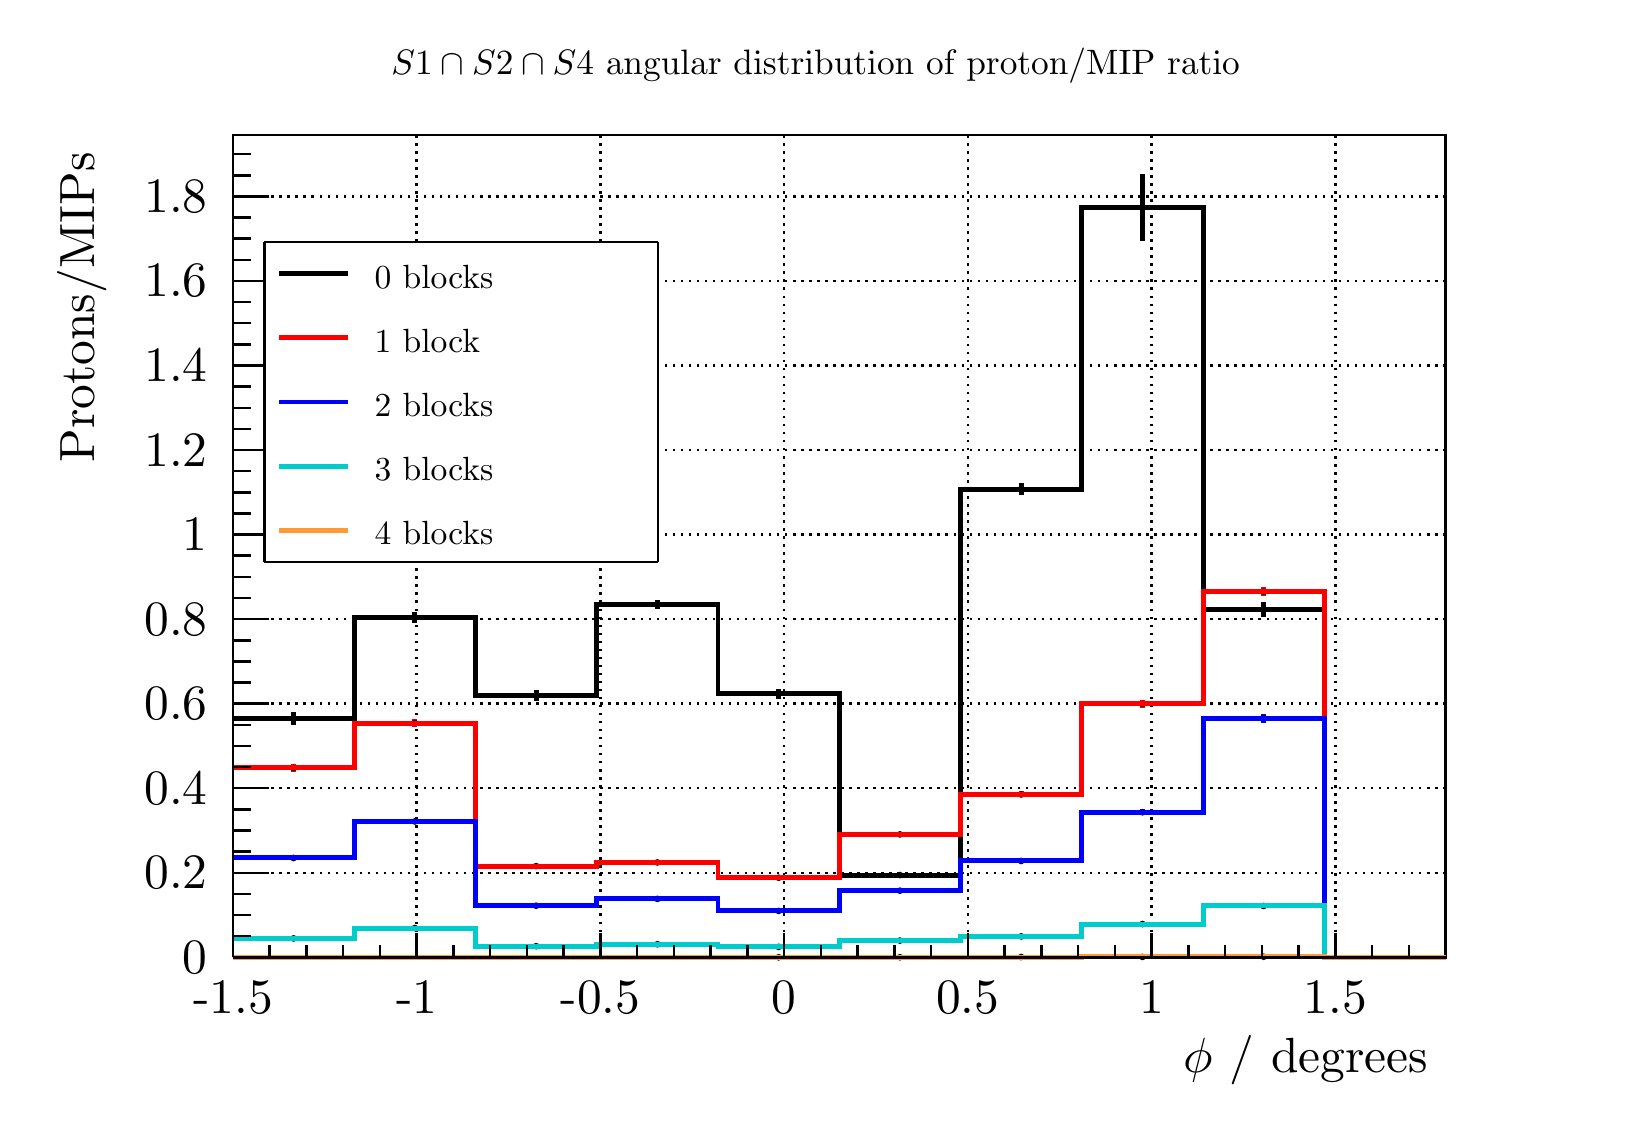
\begin{tikzpicture}
\pgfdeclareplotmark{cross} {
\pgfpathmoveto{\pgfpoint{-0.3\pgfplotmarksize}{\pgfplotmarksize}}
\pgfpathlineto{\pgfpoint{+0.3\pgfplotmarksize}{\pgfplotmarksize}}
\pgfpathlineto{\pgfpoint{+0.3\pgfplotmarksize}{0.3\pgfplotmarksize}}
\pgfpathlineto{\pgfpoint{+1\pgfplotmarksize}{0.3\pgfplotmarksize}}
\pgfpathlineto{\pgfpoint{+1\pgfplotmarksize}{-0.3\pgfplotmarksize}}
\pgfpathlineto{\pgfpoint{+0.3\pgfplotmarksize}{-0.3\pgfplotmarksize}}
\pgfpathlineto{\pgfpoint{+0.3\pgfplotmarksize}{-1.\pgfplotmarksize}}
\pgfpathlineto{\pgfpoint{-0.3\pgfplotmarksize}{-1.\pgfplotmarksize}}
\pgfpathlineto{\pgfpoint{-0.3\pgfplotmarksize}{-0.3\pgfplotmarksize}}
\pgfpathlineto{\pgfpoint{-1.\pgfplotmarksize}{-0.3\pgfplotmarksize}}
\pgfpathlineto{\pgfpoint{-1.\pgfplotmarksize}{0.3\pgfplotmarksize}}
\pgfpathlineto{\pgfpoint{-0.3\pgfplotmarksize}{0.3\pgfplotmarksize}}
\pgfpathclose
\pgfusepathqstroke
}
\pgfdeclareplotmark{cross*} {
\pgfpathmoveto{\pgfpoint{-0.3\pgfplotmarksize}{\pgfplotmarksize}}
\pgfpathlineto{\pgfpoint{+0.3\pgfplotmarksize}{\pgfplotmarksize}}
\pgfpathlineto{\pgfpoint{+0.3\pgfplotmarksize}{0.3\pgfplotmarksize}}
\pgfpathlineto{\pgfpoint{+1\pgfplotmarksize}{0.3\pgfplotmarksize}}
\pgfpathlineto{\pgfpoint{+1\pgfplotmarksize}{-0.3\pgfplotmarksize}}
\pgfpathlineto{\pgfpoint{+0.3\pgfplotmarksize}{-0.3\pgfplotmarksize}}
\pgfpathlineto{\pgfpoint{+0.3\pgfplotmarksize}{-1.\pgfplotmarksize}}
\pgfpathlineto{\pgfpoint{-0.3\pgfplotmarksize}{-1.\pgfplotmarksize}}
\pgfpathlineto{\pgfpoint{-0.3\pgfplotmarksize}{-0.3\pgfplotmarksize}}
\pgfpathlineto{\pgfpoint{-1.\pgfplotmarksize}{-0.3\pgfplotmarksize}}
\pgfpathlineto{\pgfpoint{-1.\pgfplotmarksize}{0.3\pgfplotmarksize}}
\pgfpathlineto{\pgfpoint{-0.3\pgfplotmarksize}{0.3\pgfplotmarksize}}
\pgfpathclose
\pgfusepathqfillstroke
}
\pgfdeclareplotmark{newstar} {
\pgfpathmoveto{\pgfqpoint{0pt}{\pgfplotmarksize}}
\pgfpathlineto{\pgfqpointpolar{44}{0.5\pgfplotmarksize}}
\pgfpathlineto{\pgfqpointpolar{18}{\pgfplotmarksize}}
\pgfpathlineto{\pgfqpointpolar{-20}{0.5\pgfplotmarksize}}
\pgfpathlineto{\pgfqpointpolar{-54}{\pgfplotmarksize}}
\pgfpathlineto{\pgfqpointpolar{-90}{0.5\pgfplotmarksize}}
\pgfpathlineto{\pgfqpointpolar{234}{\pgfplotmarksize}}
\pgfpathlineto{\pgfqpointpolar{198}{0.5\pgfplotmarksize}}
\pgfpathlineto{\pgfqpointpolar{162}{\pgfplotmarksize}}
\pgfpathlineto{\pgfqpointpolar{134}{0.5\pgfplotmarksize}}
\pgfpathclose
\pgfusepathqstroke
}
\pgfdeclareplotmark{newstar*} {
\pgfpathmoveto{\pgfqpoint{0pt}{\pgfplotmarksize}}
\pgfpathlineto{\pgfqpointpolar{44}{0.5\pgfplotmarksize}}
\pgfpathlineto{\pgfqpointpolar{18}{\pgfplotmarksize}}
\pgfpathlineto{\pgfqpointpolar{-20}{0.5\pgfplotmarksize}}
\pgfpathlineto{\pgfqpointpolar{-54}{\pgfplotmarksize}}
\pgfpathlineto{\pgfqpointpolar{-90}{0.5\pgfplotmarksize}}
\pgfpathlineto{\pgfqpointpolar{234}{\pgfplotmarksize}}
\pgfpathlineto{\pgfqpointpolar{198}{0.5\pgfplotmarksize}}
\pgfpathlineto{\pgfqpointpolar{162}{\pgfplotmarksize}}
\pgfpathlineto{\pgfqpointpolar{134}{0.5\pgfplotmarksize}}
\pgfpathclose
\pgfusepathqfillstroke
}
\definecolor{c}{rgb}{1,1,1};
\draw [color=c, fill=c] (0,0) rectangle (20,13.5632);
\draw [color=c, fill=c] (2.6,1.76322) rectangle (18,12.2069);
\definecolor{c}{rgb}{0,0,0};
\draw [c,line width=0.9] (2.6,1.76322) -- (2.6,12.2069) -- (18,12.2069) -- (18,1.76322) -- (2.6,1.76322);
\definecolor{c}{rgb}{1,1,1};
\draw [color=c, fill=c] (2.6,1.76322) rectangle (18,12.2069);
\definecolor{c}{rgb}{0,0,0};
\draw [c,line width=0.9] (2.6,1.76322) -- (2.6,12.2069) -- (18,12.2069) -- (18,1.76322) -- (2.6,1.76322);
\draw [c,line width=0.9] (2.6,1.76322) -- (18,1.76322);
\draw [c,dotted,line width=0.9] (2.6,12.2069) -- (2.6,1.76322);
\draw [c,dotted,line width=0.9] (4.93333,12.2069) -- (4.93333,1.76322);
\draw [c,dotted,line width=0.9] (7.26667,12.2069) -- (7.26667,1.76322);
\draw [c,dotted,line width=0.9] (9.6,12.2069) -- (9.6,1.76322);
\draw [c,dotted,line width=0.9] (11.9333,12.2069) -- (11.9333,1.76322);
\draw [c,dotted,line width=0.9] (14.2667,12.2069) -- (14.2667,1.76322);
\draw [c,dotted,line width=0.9] (16.6,12.2069) -- (16.6,1.76322);
\draw [c,dotted,line width=0.9] (16.6,12.2069) -- (16.6,1.76322);
\draw [c,line width=0.9] (2.6,1.76322) -- (2.6,12.2069);
\draw [c,dotted,line width=0.9] (18,1.76331) -- (2.6,1.76331);
\draw [c,dotted,line width=0.9] (18,2.83706) -- (2.6,2.83706);
\draw [c,dotted,line width=0.9] (18,3.91082) -- (2.6,3.91082);
\draw [c,dotted,line width=0.9] (18,4.98457) -- (2.6,4.98457);
\draw [c,dotted,line width=0.9] (18,6.05832) -- (2.6,6.05832);
\draw [c,dotted,line width=0.9] (18,7.13207) -- (2.6,7.13207);
\draw [c,dotted,line width=0.9] (18,8.20583) -- (2.6,8.20583);
\draw [c,dotted,line width=0.9] (18,9.27958) -- (2.6,9.27958);
\draw [c,dotted,line width=0.9] (18,10.3533) -- (2.6,10.3533);
\draw [c,dotted,line width=0.9] (18,11.4271) -- (2.6,11.4271);
\draw [c,dotted,line width=0.9] (18,1.76331) -- (2.6,1.76331);
\draw [c,dotted,line width=0.9] (18,11.4271) -- (2.6,11.4271);
\definecolor{c}{rgb}{0,0,0.6};
\draw [c,line width=0.9] (2.6,1.76331) -- (4.14,1.76331) -- (4.14,1.76331) -- (5.68,1.76331) -- (5.68,1.76331) -- (7.22,1.76331) -- (7.22,1.76331) -- (8.76,1.76331) -- (8.76,1.76331) -- (10.3,1.76331) -- (10.3,1.76331) -- (11.84,1.76331) --
 (11.84,1.76331) -- (13.38,1.76331) -- (13.38,1.76331) -- (14.92,1.76331) -- (14.92,1.76331) -- (16.46,1.76331) -- (16.46,1.76331) -- (18,1.76331);
\definecolor{c}{rgb}{0,0,0};
\draw [c,line width=0.9] (2.6,1.76322) -- (18,1.76322);
\draw [anchor= east] (18,0.461149) node[scale=1.78699, color=c, rotate=0]{$\phi$ / degrees};
\draw [c,line width=0.9] (2.6,2.07653) -- (2.6,1.76322);
\draw [c,line width=0.9] (3.06667,1.91987) -- (3.06667,1.76322);
\draw [c,line width=0.9] (3.53333,1.91987) -- (3.53333,1.76322);
\draw [c,line width=0.9] (4,1.91987) -- (4,1.76322);
\draw [c,line width=0.9] (4.46667,1.91987) -- (4.46667,1.76322);
\draw [c,line width=0.9] (4.93333,2.07653) -- (4.93333,1.76322);
\draw [c,line width=0.9] (5.4,1.91987) -- (5.4,1.76322);
\draw [c,line width=0.9] (5.86667,1.91987) -- (5.86667,1.76322);
\draw [c,line width=0.9] (6.33333,1.91987) -- (6.33333,1.76322);
\draw [c,line width=0.9] (6.8,1.91987) -- (6.8,1.76322);
\draw [c,line width=0.9] (7.26667,2.07653) -- (7.26667,1.76322);
\draw [c,line width=0.9] (7.73333,1.91987) -- (7.73333,1.76322);
\draw [c,line width=0.9] (8.2,1.91987) -- (8.2,1.76322);
\draw [c,line width=0.9] (8.66667,1.91987) -- (8.66667,1.76322);
\draw [c,line width=0.9] (9.13333,1.91987) -- (9.13333,1.76322);
\draw [c,line width=0.9] (9.6,2.07653) -- (9.6,1.76322);
\draw [c,line width=0.9] (10.0667,1.91987) -- (10.0667,1.76322);
\draw [c,line width=0.9] (10.5333,1.91987) -- (10.5333,1.76322);
\draw [c,line width=0.9] (11,1.91987) -- (11,1.76322);
\draw [c,line width=0.9] (11.4667,1.91987) -- (11.4667,1.76322);
\draw [c,line width=0.9] (11.9333,2.07653) -- (11.9333,1.76322);
\draw [c,line width=0.9] (12.4,1.91987) -- (12.4,1.76322);
\draw [c,line width=0.9] (12.8667,1.91987) -- (12.8667,1.76322);
\draw [c,line width=0.9] (13.3333,1.91987) -- (13.3333,1.76322);
\draw [c,line width=0.9] (13.8,1.91987) -- (13.8,1.76322);
\draw [c,line width=0.9] (14.2667,2.07653) -- (14.2667,1.76322);
\draw [c,line width=0.9] (14.7333,1.91987) -- (14.7333,1.76322);
\draw [c,line width=0.9] (15.2,1.91987) -- (15.2,1.76322);
\draw [c,line width=0.9] (15.6667,1.91987) -- (15.6667,1.76322);
\draw [c,line width=0.9] (16.1333,1.91987) -- (16.1333,1.76322);
\draw [c,line width=0.9] (16.6,2.07653) -- (16.6,1.76322);
\draw [c,line width=0.9] (16.6,2.07653) -- (16.6,1.76322);
\draw [c,line width=0.9] (17.0667,1.91987) -- (17.0667,1.76322);
\draw [c,line width=0.9] (17.5333,1.91987) -- (17.5333,1.76322);
\draw [anchor=base] (2.6,1.04437) node[scale=1.78699, color=c, rotate=0]{-1.5};
\draw [anchor=base] (4.93333,1.04437) node[scale=1.78699, color=c, rotate=0]{-1};
\draw [anchor=base] (7.26667,1.04437) node[scale=1.78699, color=c, rotate=0]{-0.5};
\draw [anchor=base] (9.6,1.04437) node[scale=1.78699, color=c, rotate=0]{0};
\draw [anchor=base] (11.9333,1.04437) node[scale=1.78699, color=c, rotate=0]{0.5};
\draw [anchor=base] (14.2667,1.04437) node[scale=1.78699, color=c, rotate=0]{1};
\draw [anchor=base] (16.6,1.04437) node[scale=1.78699, color=c, rotate=0]{1.5};
\draw [c,line width=0.9] (2.6,1.76322) -- (2.6,12.2069);
\draw [anchor= east] (0.68,12.2069) node[scale=1.78699, color=c, rotate=90]{ Protons/MIPs};
\draw [c,line width=0.9] (3.062,1.76331) -- (2.6,1.76331);
\draw [c,line width=0.9] (2.831,2.03175) -- (2.6,2.03175);
\draw [c,line width=0.9] (2.831,2.30019) -- (2.6,2.30019);
\draw [c,line width=0.9] (2.831,2.56863) -- (2.6,2.56863);
\draw [c,line width=0.9] (3.062,2.83706) -- (2.6,2.83706);
\draw [c,line width=0.9] (2.831,3.1055) -- (2.6,3.1055);
\draw [c,line width=0.9] (2.831,3.37394) -- (2.6,3.37394);
\draw [c,line width=0.9] (2.831,3.64238) -- (2.6,3.64238);
\draw [c,line width=0.9] (3.062,3.91082) -- (2.6,3.91082);
\draw [c,line width=0.9] (2.831,4.17925) -- (2.6,4.17925);
\draw [c,line width=0.9] (2.831,4.44769) -- (2.6,4.44769);
\draw [c,line width=0.9] (2.831,4.71613) -- (2.6,4.71613);
\draw [c,line width=0.9] (3.062,4.98457) -- (2.6,4.98457);
\draw [c,line width=0.9] (2.831,5.25301) -- (2.6,5.25301);
\draw [c,line width=0.9] (2.831,5.52145) -- (2.6,5.52145);
\draw [c,line width=0.9] (2.831,5.78988) -- (2.6,5.78988);
\draw [c,line width=0.9] (3.062,6.05832) -- (2.6,6.05832);
\draw [c,line width=0.9] (2.831,6.32676) -- (2.6,6.32676);
\draw [c,line width=0.9] (2.831,6.5952) -- (2.6,6.5952);
\draw [c,line width=0.9] (2.831,6.86364) -- (2.6,6.86364);
\draw [c,line width=0.9] (3.062,7.13207) -- (2.6,7.13207);
\draw [c,line width=0.9] (2.831,7.40051) -- (2.6,7.40051);
\draw [c,line width=0.9] (2.831,7.66895) -- (2.6,7.66895);
\draw [c,line width=0.9] (2.831,7.93739) -- (2.6,7.93739);
\draw [c,line width=0.9] (3.062,8.20583) -- (2.6,8.20583);
\draw [c,line width=0.9] (2.831,8.47427) -- (2.6,8.47427);
\draw [c,line width=0.9] (2.831,8.7427) -- (2.6,8.7427);
\draw [c,line width=0.9] (2.831,9.01114) -- (2.6,9.01114);
\draw [c,line width=0.9] (3.062,9.27958) -- (2.6,9.27958);
\draw [c,line width=0.9] (2.831,9.54802) -- (2.6,9.54802);
\draw [c,line width=0.9] (2.831,9.81646) -- (2.6,9.81646);
\draw [c,line width=0.9] (2.831,10.0849) -- (2.6,10.0849);
\draw [c,line width=0.9] (3.062,10.3533) -- (2.6,10.3533);
\draw [c,line width=0.9] (2.831,10.6218) -- (2.6,10.6218);
\draw [c,line width=0.9] (2.831,10.8902) -- (2.6,10.8902);
\draw [c,line width=0.9] (2.831,11.1586) -- (2.6,11.1586);
\draw [c,line width=0.9] (3.062,11.4271) -- (2.6,11.4271);
\draw [c,line width=0.9] (3.062,1.76331) -- (2.6,1.76331);
\draw [c,line width=0.9] (3.062,11.4271) -- (2.6,11.4271);
\draw [c,line width=0.9] (2.831,11.6955) -- (2.6,11.6955);
\draw [c,line width=0.9] (2.831,11.964) -- (2.6,11.964);
\draw [anchor= east] (2.5,1.76331) node[scale=1.78699, color=c, rotate=0]{0};
\draw [anchor= east] (2.5,2.83706) node[scale=1.78699, color=c, rotate=0]{0.2};
\draw [anchor= east] (2.5,3.91082) node[scale=1.78699, color=c, rotate=0]{0.4};
\draw [anchor= east] (2.5,4.98457) node[scale=1.78699, color=c, rotate=0]{0.6};
\draw [anchor= east] (2.5,6.05832) node[scale=1.78699, color=c, rotate=0]{0.8};
\draw [anchor= east] (2.5,7.13207) node[scale=1.78699, color=c, rotate=0]{1};
\draw [anchor= east] (2.5,8.20583) node[scale=1.78699, color=c, rotate=0]{1.2};
\draw [anchor= east] (2.5,9.27958) node[scale=1.78699, color=c, rotate=0]{1.4};
\draw [anchor= east] (2.5,10.3533) node[scale=1.78699, color=c, rotate=0]{1.6};
\draw [anchor= east] (2.5,11.4271) node[scale=1.78699, color=c, rotate=0]{1.8};
\draw [c,line width=1.8] (3.37,4.71121) -- (3.37,4.79669);
\draw [c,line width=1.8] (3.37,4.79669) -- (3.37,4.88216);
\foreach \P in {(3.37,4.79669)}{\draw[mark options={color=c,fill=c},mark size=2.402402pt,mark=*,mark size=1pt] plot coordinates {\P};}
\draw [c,line width=1.8] (4.91,6.01196) -- (4.91,6.07817);
\draw [c,line width=1.8] (4.91,6.07817) -- (4.91,6.14439);
\foreach \P in {(4.91,6.07817)}{\draw[mark options={color=c,fill=c},mark size=2.402402pt,mark=*,mark size=1pt] plot coordinates {\P};}
\draw [c,line width=1.8] (6.45,5.02248) -- (6.45,5.09174);
\draw [c,line width=1.8] (6.45,5.09174) -- (6.45,5.16101);
\foreach \P in {(6.45,5.09174)}{\draw[mark options={color=c,fill=c},mark size=2.402402pt,mark=*,mark size=1pt] plot coordinates {\P};}
\draw [c,line width=1.8] (7.99,6.19214) -- (7.99,6.24525);
\draw [c,line width=1.8] (7.99,6.24525) -- (7.99,6.29836);
\foreach \P in {(7.99,6.24525)}{\draw[mark options={color=c,fill=c},mark size=2.402402pt,mark=*,mark size=1pt] plot coordinates {\P};}
\draw [c,line width=1.8] (9.53,5.04647) -- (9.53,5.11033);
\draw [c,line width=1.8] (9.53,5.11033) -- (9.53,5.1742);
\foreach \P in {(9.53,5.11033)}{\draw[mark options={color=c,fill=c},mark size=2.402402pt,mark=*,mark size=1pt] plot coordinates {\P};}
\draw [c,line width=1.8] (11.07,2.77883) -- (11.07,2.80789);
\draw [c,line width=1.8] (11.07,2.80789) -- (11.07,2.83695);
\foreach \P in {(11.07,2.80789)}{\draw[mark options={color=c,fill=c},mark size=2.402402pt,mark=*,mark size=1pt] plot coordinates {\P};}
\draw [c,line width=1.8] (12.61,7.6402) -- (12.61,7.71067);
\draw [c,line width=1.8] (12.61,7.71067) -- (12.61,7.78113);
\foreach \P in {(12.61,7.71067)}{\draw[mark options={color=c,fill=c},mark size=2.402402pt,mark=*,mark size=1pt] plot coordinates {\P};}
\draw [c,line width=1.8] (14.15,10.8621) -- (14.15,11.2859);
\draw [c,line width=1.8] (14.15,11.2859) -- (14.15,11.7096);
\foreach \P in {(14.15,11.2859)}{\draw[mark options={color=c,fill=c},mark size=2.402402pt,mark=*,mark size=1pt] plot coordinates {\P};}
\draw [c,line width=1.8] (15.69,6.08849) -- (15.69,6.18452);
\draw [c,line width=1.8] (15.69,6.18452) -- (15.69,6.28056);
\foreach \P in {(15.69,6.18452)}{\draw[mark options={color=c,fill=c},mark size=2.402402pt,mark=*,mark size=1pt] plot coordinates {\P};}
\draw [c,line width=1.8] (2.6,4.79669) -- (4.14,4.79669) -- (4.14,6.07817) -- (5.68,6.07817) -- (5.68,5.09174) -- (7.22,5.09174) -- (7.22,6.24525) -- (8.76,6.24525) -- (8.76,5.11033) -- (10.3,5.11033) -- (10.3,2.80789) -- (11.84,2.80789) --
 (11.84,7.71067) -- (13.38,7.71067) -- (13.38,11.2859) -- (14.92,11.2859) -- (14.92,6.18452) -- (16.46,6.18452) -- (16.46,1.76322) -- (18,1.76322);
\definecolor{c}{rgb}{1,0,0};
\draw [c,line width=1.8] (3.37,4.11953) -- (3.37,4.1684);
\draw [c,line width=1.8] (3.37,4.1684) -- (3.37,4.21728);
\definecolor{c}{rgb}{0,0,0};
\foreach \P in {(3.37,4.1684)}{\draw[mark options={color=c,fill=c},mark size=2.402402pt,mark=*,mark size=1pt] plot coordinates {\P};}
\definecolor{c}{rgb}{1,0,0};
\draw [c,line width=1.8] (4.91,4.69275) -- (4.91,4.73893);
\draw [c,line width=1.8] (4.91,4.73893) -- (4.91,4.78512);
\definecolor{c}{rgb}{0,0,0};
\foreach \P in {(4.91,4.73893)}{\draw[mark options={color=c,fill=c},mark size=2.402402pt,mark=*,mark size=1pt] plot coordinates {\P};}
\definecolor{c}{rgb}{1,0,0};
\draw [c,line width=1.8] (6.45,2.89934) -- (6.45,2.92218);
\draw [c,line width=1.8] (6.45,2.92218) -- (6.45,2.94503);
\definecolor{c}{rgb}{0,0,0};
\foreach \P in {(6.45,2.92218)}{\draw[mark options={color=c,fill=c},mark size=2.402402pt,mark=*,mark size=1pt] plot coordinates {\P};}
\definecolor{c}{rgb}{1,0,0};
\draw [c,line width=1.8] (7.99,2.94718) -- (7.99,2.96885);
\draw [c,line width=1.8] (7.99,2.96885) -- (7.99,2.99052);
\definecolor{c}{rgb}{0,0,0};
\foreach \P in {(7.99,2.96885)}{\draw[mark options={color=c,fill=c},mark size=2.402402pt,mark=*,mark size=1pt] plot coordinates {\P};}
\definecolor{c}{rgb}{1,0,0};
\draw [c,line width=1.8] (9.53,2.75545) -- (9.53,2.77466);
\draw [c,line width=1.8] (9.53,2.77466) -- (9.53,2.79386);
\definecolor{c}{rgb}{0,0,0};
\foreach \P in {(9.53,2.77466)}{\draw[mark options={color=c,fill=c},mark size=2.402402pt,mark=*,mark size=1pt] plot coordinates {\P};}
\definecolor{c}{rgb}{1,0,0};
\draw [c,line width=1.8] (11.07,3.29785) -- (11.07,3.32473);
\draw [c,line width=1.8] (11.07,3.32473) -- (11.07,3.35162);
\definecolor{c}{rgb}{0,0,0};
\foreach \P in {(11.07,3.32473)}{\draw[mark options={color=c,fill=c},mark size=2.402402pt,mark=*,mark size=1pt] plot coordinates {\P};}
\definecolor{c}{rgb}{1,0,0};
\draw [c,line width=1.8] (12.61,3.79369) -- (12.61,3.83174);
\draw [c,line width=1.8] (12.61,3.83174) -- (12.61,3.86979);
\definecolor{c}{rgb}{0,0,0};
\foreach \P in {(12.61,3.83174)}{\draw[mark options={color=c,fill=c},mark size=2.402402pt,mark=*,mark size=1pt] plot coordinates {\P};}
\definecolor{c}{rgb}{1,0,0};
\draw [c,line width=1.8] (14.15,4.92996) -- (14.15,4.9825);
\draw [c,line width=1.8] (14.15,4.9825) -- (14.15,5.03505);
\definecolor{c}{rgb}{0,0,0};
\foreach \P in {(14.15,4.9825)}{\draw[mark options={color=c,fill=c},mark size=2.402402pt,mark=*,mark size=1pt] plot coordinates {\P};}
\definecolor{c}{rgb}{1,0,0};
\draw [c,line width=1.8] (15.69,6.35124) -- (15.69,6.40788);
\draw [c,line width=1.8] (15.69,6.40788) -- (15.69,6.46452);
\definecolor{c}{rgb}{0,0,0};
\foreach \P in {(15.69,6.40788)}{\draw[mark options={color=c,fill=c},mark size=2.402402pt,mark=*,mark size=1pt] plot coordinates {\P};}
\definecolor{c}{rgb}{1,0,0};
\draw [c,line width=1.8] (2.6,4.1684) -- (4.14,4.1684) -- (4.14,4.73893) -- (5.68,4.73893) -- (5.68,2.92218) -- (7.22,2.92218) -- (7.22,2.96885) -- (8.76,2.96885) -- (8.76,2.77466) -- (10.3,2.77466) -- (10.3,3.32473) -- (11.84,3.32473) --
 (11.84,3.83174) -- (13.38,3.83174) -- (13.38,4.9825) -- (14.92,4.9825) -- (14.92,6.40788) -- (16.46,6.40788) -- (16.46,1.76322) -- (18,1.76322);
\definecolor{c}{rgb}{0,0,1};
\draw [c,line width=1.8] (3.37,2.99342) -- (3.37,3.0254);
\draw [c,line width=1.8] (3.37,3.0254) -- (3.37,3.05738);
\definecolor{c}{rgb}{0,0,0};
\foreach \P in {(3.37,3.0254)}{\draw[mark options={color=c,fill=c},mark size=2.402402pt,mark=*,mark size=1pt] plot coordinates {\P};}
\definecolor{c}{rgb}{0,0,1};
\draw [c,line width=1.8] (4.91,3.45569) -- (4.91,3.48922);
\draw [c,line width=1.8] (4.91,3.48922) -- (4.91,3.52275);
\definecolor{c}{rgb}{0,0,0};
\foreach \P in {(4.91,3.48922)}{\draw[mark options={color=c,fill=c},mark size=2.402402pt,mark=*,mark size=1pt] plot coordinates {\P};}
\definecolor{c}{rgb}{0,0,1};
\draw [c,line width=1.8] (6.45,2.40459) -- (6.45,2.4189);
\draw [c,line width=1.8] (6.45,2.4189) -- (6.45,2.4332);
\definecolor{c}{rgb}{0,0,0};
\foreach \P in {(6.45,2.4189)}{\draw[mark options={color=c,fill=c},mark size=2.402402pt,mark=*,mark size=1pt] plot coordinates {\P};}
\definecolor{c}{rgb}{0,0,1};
\draw [c,line width=1.8] (7.99,2.49152) -- (7.99,2.50575);
\draw [c,line width=1.8] (7.99,2.50575) -- (7.99,2.51998);
\definecolor{c}{rgb}{0,0,0};
\foreach \P in {(7.99,2.50575)}{\draw[mark options={color=c,fill=c},mark size=2.402402pt,mark=*,mark size=1pt] plot coordinates {\P};}
\definecolor{c}{rgb}{0,0,1};
\draw [c,line width=1.8] (9.53,2.34143) -- (9.53,2.35363);
\draw [c,line width=1.8] (9.53,2.35363) -- (9.53,2.36583);
\definecolor{c}{rgb}{0,0,0};
\foreach \P in {(9.53,2.35363)}{\draw[mark options={color=c,fill=c},mark size=2.402402pt,mark=*,mark size=1pt] plot coordinates {\P};}
\definecolor{c}{rgb}{0,0,1};
\draw [c,line width=1.8] (11.07,2.59294) -- (11.07,2.61003);
\draw [c,line width=1.8] (11.07,2.61003) -- (11.07,2.62713);
\definecolor{c}{rgb}{0,0,0};
\foreach \P in {(11.07,2.61003)}{\draw[mark options={color=c,fill=c},mark size=2.402402pt,mark=*,mark size=1pt] plot coordinates {\P};}
\definecolor{c}{rgb}{0,0,1};
\draw [c,line width=1.8] (12.61,2.96164) -- (12.61,2.98755);
\draw [c,line width=1.8] (12.61,2.98755) -- (12.61,3.01347);
\definecolor{c}{rgb}{0,0,0};
\foreach \P in {(12.61,2.98755)}{\draw[mark options={color=c,fill=c},mark size=2.402402pt,mark=*,mark size=1pt] plot coordinates {\P};}
\definecolor{c}{rgb}{0,0,1};
\draw [c,line width=1.8] (14.15,3.56827) -- (14.15,3.60626);
\draw [c,line width=1.8] (14.15,3.60626) -- (14.15,3.64424);
\definecolor{c}{rgb}{0,0,0};
\foreach \P in {(14.15,3.60626)}{\draw[mark options={color=c,fill=c},mark size=2.402402pt,mark=*,mark size=1pt] plot coordinates {\P};}
\definecolor{c}{rgb}{0,0,1};
\draw [c,line width=1.8] (15.69,4.74022) -- (15.69,4.79919);
\draw [c,line width=1.8] (15.69,4.79919) -- (15.69,4.85817);
\definecolor{c}{rgb}{0,0,0};
\foreach \P in {(15.69,4.79919)}{\draw[mark options={color=c,fill=c},mark size=2.402402pt,mark=*,mark size=1pt] plot coordinates {\P};}
\definecolor{c}{rgb}{0,0,1};
\draw [c,line width=1.8] (2.6,3.0254) -- (4.14,3.0254) -- (4.14,3.48922) -- (5.68,3.48922) -- (5.68,2.4189) -- (7.22,2.4189) -- (7.22,2.50575) -- (8.76,2.50575) -- (8.76,2.35363) -- (10.3,2.35363) -- (10.3,2.61003) -- (11.84,2.61003) --
 (11.84,2.98755) -- (13.38,2.98755) -- (13.38,3.60626) -- (14.92,3.60626) -- (14.92,4.79919) -- (16.46,4.79919) -- (16.46,1.76322) -- (18,1.76322);
\definecolor{c}{rgb}{0,0.8,0.8};
\draw [c,line width=1.8] (3.37,1.98645) -- (3.37,2.00382);
\draw [c,line width=1.8] (3.37,2.00382) -- (3.37,2.02119);
\definecolor{c}{rgb}{0,0,0};
\foreach \P in {(3.37,2.00382)}{\draw[mark options={color=c,fill=c},mark size=2.402402pt,mark=*,mark size=1pt] plot coordinates {\P};}
\definecolor{c}{rgb}{0,0.8,0.8};
\draw [c,line width=1.8] (4.91,2.1156) -- (4.91,2.1351);
\draw [c,line width=1.8] (4.91,2.1351) -- (4.91,2.1546);
\definecolor{c}{rgb}{0,0,0};
\foreach \P in {(4.91,2.1351)}{\draw[mark options={color=c,fill=c},mark size=2.402402pt,mark=*,mark size=1pt] plot coordinates {\P};}
\definecolor{c}{rgb}{0,0.8,0.8};
\draw [c,line width=1.8] (6.45,1.89731) -- (6.45,1.90524);
\draw [c,line width=1.8] (6.45,1.90524) -- (6.45,1.91317);
\definecolor{c}{rgb}{0,0,0};
\foreach \P in {(6.45,1.90524)}{\draw[mark options={color=c,fill=c},mark size=2.402402pt,mark=*,mark size=1pt] plot coordinates {\P};}
\definecolor{c}{rgb}{0,0.8,0.8};
\draw [c,line width=1.8] (7.99,1.92127) -- (7.99,1.92926);
\draw [c,line width=1.8] (7.99,1.92926) -- (7.99,1.93725);
\definecolor{c}{rgb}{0,0,0};
\foreach \P in {(7.99,1.92926)}{\draw[mark options={color=c,fill=c},mark size=2.402402pt,mark=*,mark size=1pt] plot coordinates {\P};}
\definecolor{c}{rgb}{0,0.8,0.8};
\draw [c,line width=1.8] (9.53,1.88965) -- (9.53,1.89653);
\draw [c,line width=1.8] (9.53,1.89653) -- (9.53,1.90341);
\definecolor{c}{rgb}{0,0,0};
\foreach \P in {(9.53,1.89653)}{\draw[mark options={color=c,fill=c},mark size=2.402402pt,mark=*,mark size=1pt] plot coordinates {\P};}
\definecolor{c}{rgb}{0,0.8,0.8};
\draw [c,line width=1.8] (11.07,1.96599) -- (11.07,1.97605);
\draw [c,line width=1.8] (11.07,1.97605) -- (11.07,1.98611);
\definecolor{c}{rgb}{0,0,0};
\foreach \P in {(11.07,1.97605)}{\draw[mark options={color=c,fill=c},mark size=2.402402pt,mark=*,mark size=1pt] plot coordinates {\P};}
\definecolor{c}{rgb}{0,0.8,0.8};
\draw [c,line width=1.8] (12.61,2.01471) -- (12.61,2.0295);
\draw [c,line width=1.8] (12.61,2.0295) -- (12.61,2.04429);
\definecolor{c}{rgb}{0,0,0};
\foreach \P in {(12.61,2.0295)}{\draw[mark options={color=c,fill=c},mark size=2.402402pt,mark=*,mark size=1pt] plot coordinates {\P};}
\definecolor{c}{rgb}{0,0.8,0.8};
\draw [c,line width=1.8] (14.15,2.16322) -- (14.15,2.18639);
\draw [c,line width=1.8] (14.15,2.18639) -- (14.15,2.20956);
\definecolor{c}{rgb}{0,0,0};
\foreach \P in {(14.15,2.18639)}{\draw[mark options={color=c,fill=c},mark size=2.402402pt,mark=*,mark size=1pt] plot coordinates {\P};}
\definecolor{c}{rgb}{0,0.8,0.8};
\draw [c,line width=1.8] (15.69,2.37467) -- (15.69,2.41691);
\draw [c,line width=1.8] (15.69,2.41691) -- (15.69,2.45915);
\definecolor{c}{rgb}{0,0,0};
\foreach \P in {(15.69,2.41691)}{\draw[mark options={color=c,fill=c},mark size=2.402402pt,mark=*,mark size=1pt] plot coordinates {\P};}
\definecolor{c}{rgb}{0,0.8,0.8};
\draw [c,line width=1.8] (2.6,2.00382) -- (4.14,2.00382) -- (4.14,2.1351) -- (5.68,2.1351) -- (5.68,1.90524) -- (7.22,1.90524) -- (7.22,1.92926) -- (8.76,1.92926) -- (8.76,1.89653) -- (10.3,1.89653) -- (10.3,1.97605) -- (11.84,1.97605) --
 (11.84,2.0295) -- (13.38,2.0295) -- (13.38,2.18639) -- (14.92,2.18639) -- (14.92,2.41691) -- (16.46,2.41691) -- (16.46,1.76322) -- (18,1.76322);
\definecolor{c}{rgb}{1,0.6,0.2};
\draw [c,line width=1.8] (9.53,1.76322) -- (9.53,1.76399);
\draw [c,line width=1.8] (9.53,1.76399) -- (9.53,1.76476);
\definecolor{c}{rgb}{0,0,0};
\foreach \P in {(9.53,1.76399)}{\draw[mark options={color=c,fill=c},mark size=2.402402pt,mark=*,mark size=1pt] plot coordinates {\P};}
\definecolor{c}{rgb}{1,0.6,0.2};
\draw [c,line width=1.8] (11.07,1.76366) -- (11.07,1.76464);
\draw [c,line width=1.8] (11.07,1.76464) -- (11.07,1.76562);
\definecolor{c}{rgb}{0,0,0};
\foreach \P in {(11.07,1.76464)}{\draw[mark options={color=c,fill=c},mark size=2.402402pt,mark=*,mark size=1pt] plot coordinates {\P};}
\definecolor{c}{rgb}{1,0.6,0.2};
\draw [c,line width=1.8] (12.61,1.76559) -- (12.61,1.76699);
\draw [c,line width=1.8] (12.61,1.76699) -- (12.61,1.7684);
\definecolor{c}{rgb}{0,0,0};
\foreach \P in {(12.61,1.76699)}{\draw[mark options={color=c,fill=c},mark size=2.402402pt,mark=*,mark size=1pt] plot coordinates {\P};}
\definecolor{c}{rgb}{1,0.6,0.2};
\draw [c,line width=1.8] (14.15,1.76701) -- (14.15,1.76884);
\draw [c,line width=1.8] (14.15,1.76884) -- (14.15,1.77066);
\definecolor{c}{rgb}{0,0,0};
\foreach \P in {(14.15,1.76884)}{\draw[mark options={color=c,fill=c},mark size=2.402402pt,mark=*,mark size=1pt] plot coordinates {\P};}
\definecolor{c}{rgb}{1,0.6,0.2};
\draw [c,line width=1.8] (15.69,1.7683) -- (15.69,1.77128);
\draw [c,line width=1.8] (15.69,1.77128) -- (15.69,1.77426);
\definecolor{c}{rgb}{0,0,0};
\foreach \P in {(15.69,1.77128)}{\draw[mark options={color=c,fill=c},mark size=2.402402pt,mark=*,mark size=1pt] plot coordinates {\P};}
\definecolor{c}{rgb}{1,0.6,0.2};
\draw [c,line width=1.8] (2.6,1.76322) -- (4.14,1.76322) -- (4.14,1.76322) -- (5.68,1.76322) -- (5.68,1.76322) -- (7.22,1.76322) -- (7.22,1.76322) -- (8.76,1.76322) -- (8.76,1.76322) -- (10.3,1.76322) -- (10.3,1.76464) -- (11.84,1.76464) --
 (11.84,1.76699) -- (13.38,1.76699) -- (13.38,1.76884) -- (14.92,1.76884) -- (14.92,1.77128) -- (16.46,1.77128) -- (16.46,1.76322) -- (18,1.76322);
\definecolor{c}{rgb}{0,0,0};
\draw [c,line width=0.9] (2.6,1.76322) -- (18,1.76322);
\draw [c,line width=0.9] (2.6,2.07653) -- (2.6,1.76322);
\draw [c,line width=0.9] (3.06667,1.91987) -- (3.06667,1.76322);
\draw [c,line width=0.9] (3.53333,1.91987) -- (3.53333,1.76322);
\draw [c,line width=0.9] (4,1.91987) -- (4,1.76322);
\draw [c,line width=0.9] (4.46667,1.91987) -- (4.46667,1.76322);
\draw [c,line width=0.9] (4.93333,2.07653) -- (4.93333,1.76322);
\draw [c,line width=0.9] (5.4,1.91987) -- (5.4,1.76322);
\draw [c,line width=0.9] (5.86667,1.91987) -- (5.86667,1.76322);
\draw [c,line width=0.9] (6.33333,1.91987) -- (6.33333,1.76322);
\draw [c,line width=0.9] (6.8,1.91987) -- (6.8,1.76322);
\draw [c,line width=0.9] (7.26667,2.07653) -- (7.26667,1.76322);
\draw [c,line width=0.9] (7.73333,1.91987) -- (7.73333,1.76322);
\draw [c,line width=0.9] (8.2,1.91987) -- (8.2,1.76322);
\draw [c,line width=0.9] (8.66667,1.91987) -- (8.66667,1.76322);
\draw [c,line width=0.9] (9.13333,1.91987) -- (9.13333,1.76322);
\draw [c,line width=0.9] (9.6,2.07653) -- (9.6,1.76322);
\draw [c,line width=0.9] (10.0667,1.91987) -- (10.0667,1.76322);
\draw [c,line width=0.9] (10.5333,1.91987) -- (10.5333,1.76322);
\draw [c,line width=0.9] (11,1.91987) -- (11,1.76322);
\draw [c,line width=0.9] (11.4667,1.91987) -- (11.4667,1.76322);
\draw [c,line width=0.9] (11.9333,2.07653) -- (11.9333,1.76322);
\draw [c,line width=0.9] (12.4,1.91987) -- (12.4,1.76322);
\draw [c,line width=0.9] (12.8667,1.91987) -- (12.8667,1.76322);
\draw [c,line width=0.9] (13.3333,1.91987) -- (13.3333,1.76322);
\draw [c,line width=0.9] (13.8,1.91987) -- (13.8,1.76322);
\draw [c,line width=0.9] (14.2667,2.07653) -- (14.2667,1.76322);
\draw [c,line width=0.9] (14.7333,1.91987) -- (14.7333,1.76322);
\draw [c,line width=0.9] (15.2,1.91987) -- (15.2,1.76322);
\draw [c,line width=0.9] (15.6667,1.91987) -- (15.6667,1.76322);
\draw [c,line width=0.9] (16.1333,1.91987) -- (16.1333,1.76322);
\draw [c,line width=0.9] (16.6,2.07653) -- (16.6,1.76322);
\draw [c,line width=0.9] (16.6,2.07653) -- (16.6,1.76322);
\draw [c,line width=0.9] (17.0667,1.91987) -- (17.0667,1.76322);
\draw [c,line width=0.9] (17.5333,1.91987) -- (17.5333,1.76322);
\draw [c,line width=0.9] (2.6,1.76322) -- (2.6,12.2069);
\draw [c,line width=0.9] (3.062,1.76331) -- (2.6,1.76331);
\draw [c,line width=0.9] (2.831,2.03175) -- (2.6,2.03175);
\draw [c,line width=0.9] (2.831,2.30019) -- (2.6,2.30019);
\draw [c,line width=0.9] (2.831,2.56863) -- (2.6,2.56863);
\draw [c,line width=0.9] (3.062,2.83706) -- (2.6,2.83706);
\draw [c,line width=0.9] (2.831,3.1055) -- (2.6,3.1055);
\draw [c,line width=0.9] (2.831,3.37394) -- (2.6,3.37394);
\draw [c,line width=0.9] (2.831,3.64238) -- (2.6,3.64238);
\draw [c,line width=0.9] (3.062,3.91082) -- (2.6,3.91082);
\draw [c,line width=0.9] (2.831,4.17925) -- (2.6,4.17925);
\draw [c,line width=0.9] (2.831,4.44769) -- (2.6,4.44769);
\draw [c,line width=0.9] (2.831,4.71613) -- (2.6,4.71613);
\draw [c,line width=0.9] (3.062,4.98457) -- (2.6,4.98457);
\draw [c,line width=0.9] (2.831,5.25301) -- (2.6,5.25301);
\draw [c,line width=0.9] (2.831,5.52145) -- (2.6,5.52145);
\draw [c,line width=0.9] (2.831,5.78988) -- (2.6,5.78988);
\draw [c,line width=0.9] (3.062,6.05832) -- (2.6,6.05832);
\draw [c,line width=0.9] (2.831,6.32676) -- (2.6,6.32676);
\draw [c,line width=0.9] (2.831,6.5952) -- (2.6,6.5952);
\draw [c,line width=0.9] (2.831,6.86364) -- (2.6,6.86364);
\draw [c,line width=0.9] (3.062,7.13207) -- (2.6,7.13207);
\draw [c,line width=0.9] (2.831,7.40051) -- (2.6,7.40051);
\draw [c,line width=0.9] (2.831,7.66895) -- (2.6,7.66895);
\draw [c,line width=0.9] (2.831,7.93739) -- (2.6,7.93739);
\draw [c,line width=0.9] (3.062,8.20583) -- (2.6,8.20583);
\draw [c,line width=0.9] (2.831,8.47427) -- (2.6,8.47427);
\draw [c,line width=0.9] (2.831,8.7427) -- (2.6,8.7427);
\draw [c,line width=0.9] (2.831,9.01114) -- (2.6,9.01114);
\draw [c,line width=0.9] (3.062,9.27958) -- (2.6,9.27958);
\draw [c,line width=0.9] (2.831,9.54802) -- (2.6,9.54802);
\draw [c,line width=0.9] (2.831,9.81646) -- (2.6,9.81646);
\draw [c,line width=0.9] (2.831,10.0849) -- (2.6,10.0849);
\draw [c,line width=0.9] (3.062,10.3533) -- (2.6,10.3533);
\draw [c,line width=0.9] (2.831,10.6218) -- (2.6,10.6218);
\draw [c,line width=0.9] (2.831,10.8902) -- (2.6,10.8902);
\draw [c,line width=0.9] (2.831,11.1586) -- (2.6,11.1586);
\draw [c,line width=0.9] (3.062,11.4271) -- (2.6,11.4271);
\draw [c,line width=0.9] (3.062,1.76331) -- (2.6,1.76331);
\draw [c,line width=0.9] (3.062,11.4271) -- (2.6,11.4271);
\draw [c,line width=0.9] (2.831,11.6955) -- (2.6,11.6955);
\draw [c,line width=0.9] (2.831,11.964) -- (2.6,11.964);
\draw (10,13.0816) node[scale=1.27642, color=c, rotate=0]{$S1 \cap S2 \cap S4$ angular distribution of proton/MIP ratio};
\definecolor{c}{rgb}{1,1,1};
\draw [color=c, fill=c] (3,6.78161) rectangle (8,10.8506);
\definecolor{c}{rgb}{0,0,0};
\draw [c,line width=0.9] (3,6.78161) -- (8,6.78161);
\draw [c,line width=0.9] (8,6.78161) -- (8,10.8506);
\draw [c,line width=0.9] (8,10.8506) -- (3,10.8506);
\draw [c,line width=0.9] (3,10.8506) -- (3,6.78161);
\draw [anchor=base west] (4.25,10.2606) node[scale=1.2126, color=c, rotate=0]{0 blocks};
\draw [c,line width=1.8] (3.1875,10.4437) -- (4.0625,10.4437);
\draw [anchor=base west] (4.25,9.44678) node[scale=1.2126, color=c, rotate=0]{1 block};
\definecolor{c}{rgb}{1,0,0};
\draw [c,line width=1.8] (3.1875,9.62988) -- (4.0625,9.62988);
\definecolor{c}{rgb}{0,0,0};
\draw [anchor=base west] (4.25,8.63299) node[scale=1.2126, color=c, rotate=0]{2 blocks};
\definecolor{c}{rgb}{0,0,1};
\draw [c,line width=1.8] (3.1875,8.81609) -- (4.0625,8.81609);
\definecolor{c}{rgb}{0,0,0};
\draw [anchor=base west] (4.25,7.8192) node[scale=1.2126, color=c, rotate=0]{3 blocks};
\definecolor{c}{rgb}{0,0.8,0.8};
\draw [c,line width=1.8] (3.1875,8.0023) -- (4.0625,8.0023);
\definecolor{c}{rgb}{0,0,0};
\draw [anchor=base west] (4.25,7.0054) node[scale=1.2126, color=c, rotate=0]{4 blocks};
\definecolor{c}{rgb}{1,0.6,0.2};
\draw [c,line width=1.8] (3.1875,7.18851) -- (4.0625,7.18851);
\end{tikzpicture}

	    	\end{adjustbox}
    		\caption{Proton/MIP ratio in $S_{4}$ for varying numbers of moderator blocks as a function of vertical off-axis angle, as measured from $S_{1}$}
    		\label{fig:propiratio_s4_vert}
    	\end{minipage}	
   	\end{figure}
   
	

Exact UToF and DToF figures TBD